\section{Introduction}
\label{implementation_testing_introduction}
In this chapter we will present the results of the implementation and validation process used for developing the predictive model described in chapter \ref{chapter_theory_modelling}. Indeed, relevant to our approach for approximating the latent motivational state of an individual is to have a model able to reliably predict the intensity of future behaviour (i.e., future engagement in a videogame context) given the history of interactions between an individual and a potential rewarding object (i.e., a videogame). 

To achieve this, we adopted a variation of bottom-up iterative model building \cite{gelman2020bayesian} in which first the simplest version of a model is designed, built and evaluated and then, based on performance and addition theoretical assumptions, a new improved version of the same model is proposed. At each stage of the process we evaluated the new version of the model against alternative approaches in order to test for hypotheses stated in the model design stage. 

Each section of this chapter corresponds to a different version of the model and will have the following structure.: In \textbf{Model Design} we will state the task the model is trying to solve, the design of such model and the theoretical assumptions that informed the design. In \textbf{Data} we will describe the dataset used for evaluating the performance of our model along with any data-related processing. In \textbf{Model Comparison} we will outline the alternative approaches against which the current model is compared and the various procedures and statistical analyses employed. In \textbf{Results} we will report the outcomes of the model comparison procedure with particular focus on the assessment of the predictive accuracy. In \textbf{Model Criticism} we will discuss what presented in the results section,in light of the theoretical assumptions used when designing the model, and highlight potential improvements to be carried out in the subsequent stage of the model building process. 

Despite the \textbf{Model Comparison} stage differed slightly between the various stages of the model building process, a common experimental pipeline was adopted. We can see a graphical representation of the latter in Figure 

\ref{fig: pipeline_eval}
\begin{figure}[h]
  \centering
  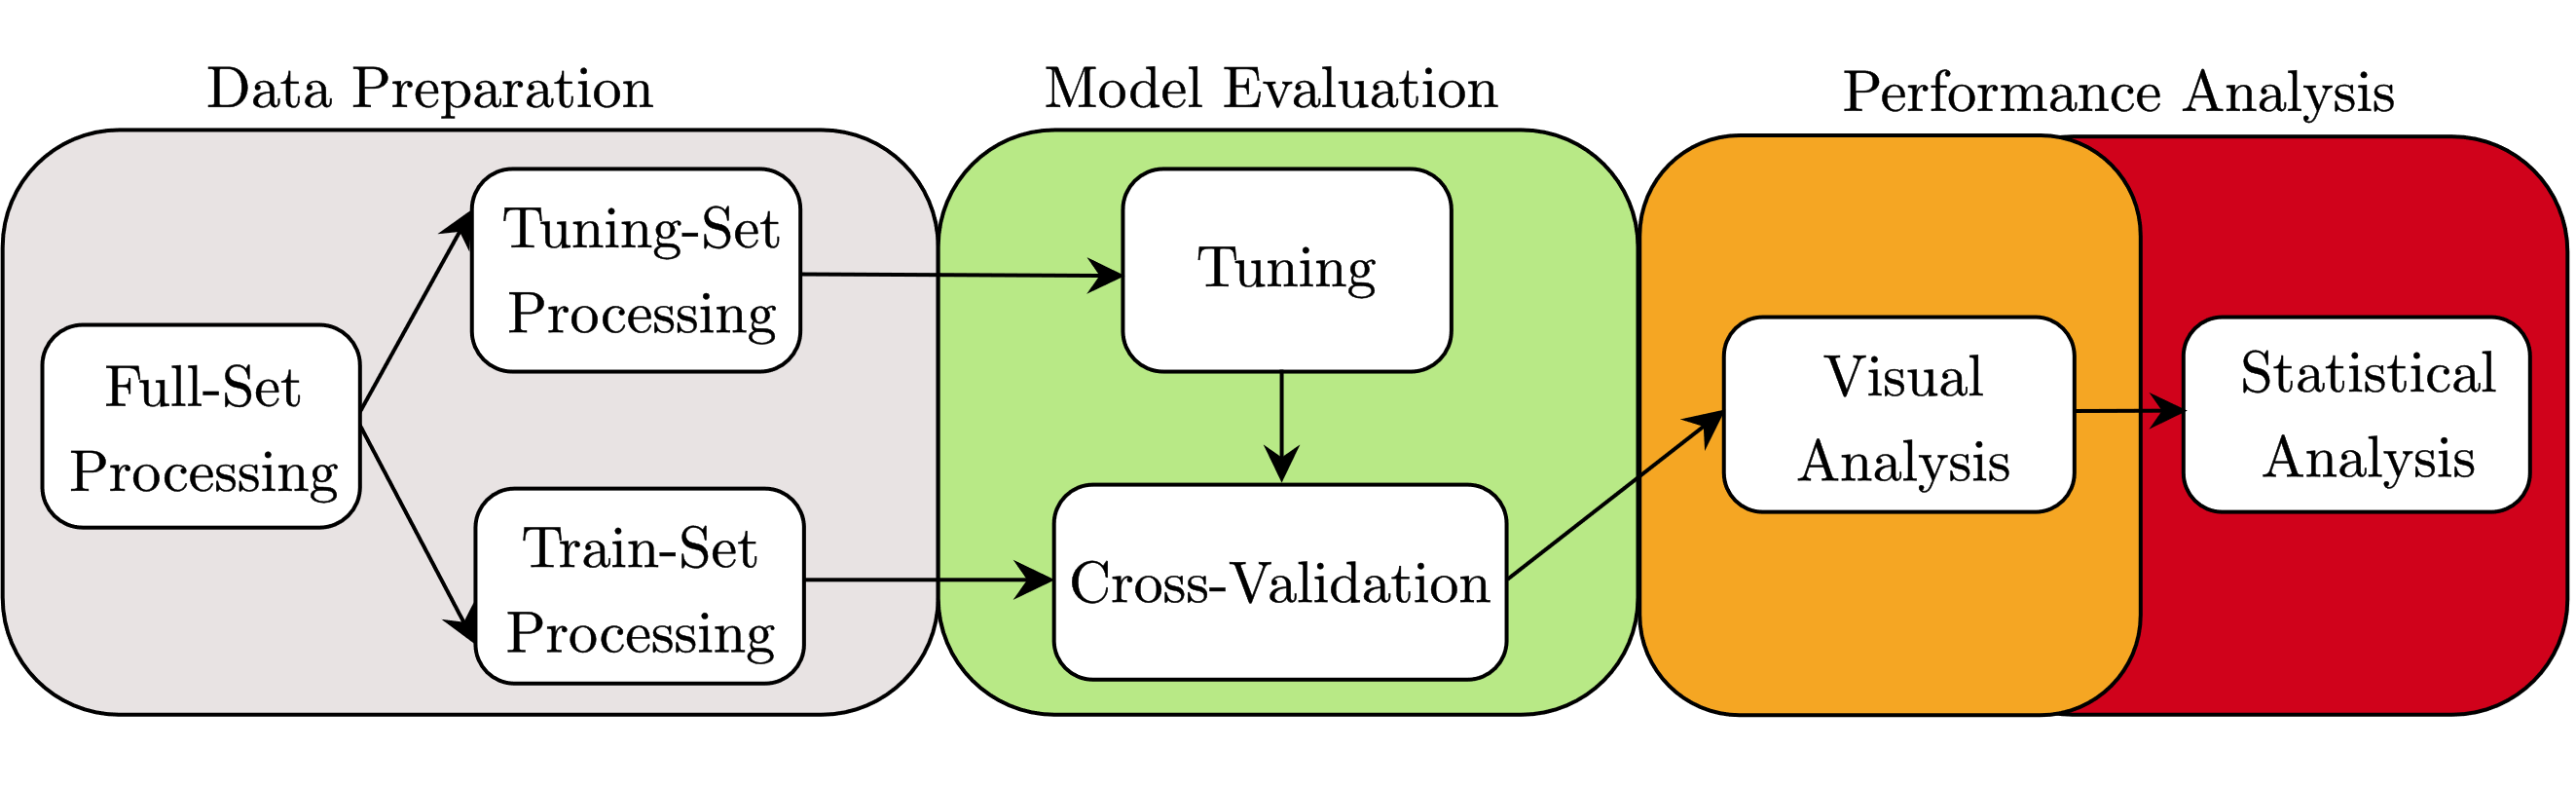
\includegraphics[width=\textwidth]{images/chapter_3/pipeline_eval.png}
    \caption[\textbf{Model implementation experimental pipeline}]{Arrows indicate the flow of the pipeline. Big coloured blocks are major pipeline steps, white rectangles indicate sub-tasks within each step.}
    \label{fig: pipeline_eval}
\end{figure}

\section{Joint Prediction of Long Term Behavioural Intensity}
\label{model_architecture_1}
In the first iteration of our model building process we focused on implementing and testing some of the core theoretical assumptions presented in chapter \ref{chapter_theory_modelling}, namely the importance of modelling temporal and non-linear dynamics in the interactions between an individual and a videogame. 

The experimental task used for this purpose aimed at predicting the long term intensity of interactions between an individual and a videogame given a set of behavioural metrics recorded during an initial observation period. Here, the observation period is defined as a small sequence of initial interactions between an individual and a videogame. In this specific context, we used churn and survival time as behavioural proxies for the expected intensity of future interactions. We briefly introduced these two concepts in section \ref{engagement_prediction}. More formally we can say that given a sequence of interactions with associated behavioural intensity $B_{t_1 : T}$, survival time is the amount of expected future playing activity at a given point $t_n$ \cite{ perianez2016churn, demediuk2018player, bertens2017games, kim2017churn, viljanen2018playtime}

\begin{equation}
\label{eq_survival}
    survival = \sum_{t_n}^{T}B_t
\end{equation}

while churn is the probability of observing a terminal event $C$ (usually formulated as a prolonged period of inactivity from the individual) after a given point $t_n$ \cite{hadiji2014predicting,runge2014churn, drachen2016rapid,milovsevic2017early, kim2017churn}.

\begin{equation}
\label{eq_churn}
    churn = \sum_{t_n}^{T}C_n = 1
\end{equation}

here the interactions going from $t_1: t_n$ define our observation period. It has to be noted that this task can be viewed as a special case of the more general formulation presented in section \ref{td_to_supervised}, precisely 

\begin{equation}
\label{rnn_1_exp}
   \mathbb{E}[B_{t_n : T}] = \mathbb{E}[B_{t_n : T}]
\end{equation}

and correspond to predicting extinction and future amount of sustained engagement after observing a handful of interactions following the point of engagement (according to O'Brien et al. \cite{o2008user} framework presented in section \ref{eng_reward_motivation}). 

Given this experimental context, the hypotheses that we wanted to evaluate in order to support our modelling intuitions were the following:
\begin{enumerate}
    \item Leveraging all the information provided by the behavioural data defining the observation period is required for achieving higher predictive power.
    \item Approaches able to account for non-linear interactions in the considered behavioural metrics can outperform simpler additive models.
    \item The ability to model the type of sequential dynamics presented in section \ref{td_to_supervised} can have a positive effect on the predictive performance.
    \item It is possible to have a single model jointly predict the considered metrics of long term behavioural intensity without any loss of predictive accuracy.
    \item It is possible to have a single model performing the predictive task simultaneously across a wide range of games.
\end{enumerate}

\subsection{Model Design}
\label{model_design_1}
The first iteration of our ANN architecture, loosely inspired by the winning entry  of the 2018 CIG 2018 churn and survival time competition \cite{lee2018game}, aimed to jointly predict survival time and churn probability across a set of 6 different game contexts. This architecture, the `Bifurcating Model' (BM), is illustrated in Fig. \ref{fig: rnn_1}. 
\begin{figure}[ht]
\begin{center}
\begin{adjustbox}{width=0.7\textwidth}



\tikzset{every picture/.style={line width=0.75pt}} %set default line width to 0.75pt        

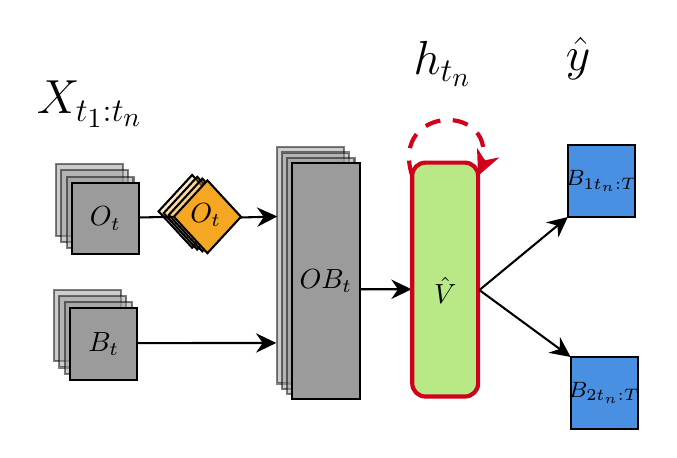
\begin{tikzpicture}[x=0.75pt,y=0.75pt,yscale=-1,xscale=1]
%uncomment if require: \path (0,300); %set diagram left start at 0, and has height of 300

%Shape: Diamond [id:dp06877884521197963] 
\draw  [fill={rgb, 255:red, 245; green, 166; blue, 35 }  ,fill opacity=0.25 ] (263.6,117.28) -- (279.77,134.81) -- (263.6,152.33) -- (247.43,134.81) -- cycle ;
%Shape: Diamond [id:dp5019197402707816] 
\draw  [fill={rgb, 255:red, 245; green, 166; blue, 35 }  ,fill opacity=0.25 ] (266.05,118.16) -- (282.22,135.68) -- (266.05,153.2) -- (249.89,135.68) -- cycle ;
%Shape: Diamond [id:dp6628494024847519] 
\draw  [fill={rgb, 255:red, 245; green, 166; blue, 35 }  ,fill opacity=0.25 ] (268.51,119.04) -- (284.68,136.56) -- (268.51,154.08) -- (252.34,136.56) -- cycle ;
%Shape: Rectangle [id:dp8304682723722553] 
\draw  [color={rgb, 255:red, 0; green, 0; blue, 0 }  ,draw opacity=0.5 ][fill={rgb, 255:red, 155; green, 155; blue, 155 }  ,fill opacity=0.5 ] (304.41,104.01) -- (336.92,104.01) -- (336.92,217.74) -- (304.41,217.74) -- cycle ;
%Shape: Rectangle [id:dp33657106031779216] 
\draw  [color={rgb, 255:red, 0; green, 0; blue, 0 }  ,draw opacity=0.5 ][fill={rgb, 255:red, 155; green, 155; blue, 155 }  ,fill opacity=0.5 ] (306.86,106.47) -- (339.38,106.47) -- (339.38,220.2) -- (306.86,220.2) -- cycle ;
%Shape: Rectangle [id:dp6698304713342962] 
\draw  [color={rgb, 255:red, 0; green, 0; blue, 0 }  ,draw opacity=0.5 ][fill={rgb, 255:red, 155; green, 155; blue, 155 }  ,fill opacity=0.5 ] (309.32,108.93) -- (341.84,108.93) -- (341.84,222.66) -- (309.32,222.66) -- cycle ;
%Shape: Diamond [id:dp7704333366065277] 
\draw  [fill={rgb, 255:red, 245; green, 166; blue, 35 }  ,fill opacity=1 ] (270.97,119.91) -- (287.13,137.43) -- (270.97,154.96) -- (254.8,137.43) -- cycle ;
%Straight Lines [id:da34159449213041837] 
\draw    (286.94,137.77) -- (301.65,137.38) ;
\draw [shift={(304.65,137.3)}, rotate = 178.49] [fill={rgb, 255:red, 0; green, 0; blue, 0 }  ][line width=0.08]  [draw opacity=0] (9.82,-4.72) -- (0,0) -- (9.82,4.72) -- (6.52,0) -- cycle    ;
%Straight Lines [id:da8208338090000002] 
\draw [fill={rgb, 255:red, 155; green, 155; blue, 155 }  ,fill opacity=1 ]   (215.09,198.3) -- (301.13,198.22) ;
\draw [shift={(304.13,198.22)}, rotate = 179.95] [fill={rgb, 255:red, 0; green, 0; blue, 0 }  ][line width=0.08]  [draw opacity=0] (9.82,-4.72) -- (0,0) -- (9.82,4.72) -- (6.52,0) -- cycle    ;
%Straight Lines [id:da7791621502079311] 
\draw [fill={rgb, 255:red, 155; green, 155; blue, 155 }  ,fill opacity=1 ]   (336.42,172.36) -- (366.33,172.35) ;
\draw [shift={(369.33,172.35)}, rotate = 179.97] [fill={rgb, 255:red, 0; green, 0; blue, 0 }  ][line width=0.08]  [draw opacity=0] (9.82,-4.72) -- (0,0) -- (9.82,4.72) -- (6.52,0) -- cycle    ;
%Shape: Rectangle [id:dp3847312278870677] 
\draw  [color={rgb, 255:red, 0; green, 0; blue, 0 }  ,draw opacity=0.5 ][fill={rgb, 255:red, 155; green, 155; blue, 155 }  ,fill opacity=0.5 ] (197.01,172.53) -- (229.26,172.53) -- (229.26,207.05) -- (197.01,207.05) -- cycle ;
%Shape: Rectangle [id:dp5169374919332619] 
\draw  [color={rgb, 255:red, 0; green, 0; blue, 0 }  ,draw opacity=0.5 ][fill={rgb, 255:red, 155; green, 155; blue, 155 }  ,fill opacity=0.5 ] (199.63,175.51) -- (231.88,175.51) -- (231.88,210.03) -- (199.63,210.03) -- cycle ;
%Shape: Rectangle [id:dp7025889851900418] 
\draw  [color={rgb, 255:red, 0; green, 0; blue, 0 }  ,draw opacity=0.5 ][fill={rgb, 255:red, 155; green, 155; blue, 155 }  ,fill opacity=0.5 ] (202.27,178.56) -- (234.53,178.56) -- (234.53,213.08) -- (202.27,213.08) -- cycle ;
%Shape: Rectangle [id:dp34989838660273853] 
\draw  [fill={rgb, 255:red, 155; green, 155; blue, 155 }  ,fill opacity=1 ] (204.86,181.5) -- (237.11,181.5) -- (237.11,216.02) -- (204.86,216.02) -- cycle ;
%Shape: Rectangle [id:dp10413248734443492] 
\draw  [fill={rgb, 255:red, 155; green, 155; blue, 155 }  ,fill opacity=1 ] (311.77,111.39) -- (344.29,111.39) -- (344.29,225.12) -- (311.77,225.12) -- cycle ;
%Shape: Rectangle [id:dp5251277777045114] 
\draw  [color={rgb, 255:red, 0; green, 0; blue, 0 }  ,draw opacity=0.5 ][fill={rgb, 255:red, 155; green, 155; blue, 155 }  ,fill opacity=0.5 ] (197.83,112.08) -- (230.08,112.08) -- (230.08,146.6) -- (197.83,146.6) -- cycle ;
%Shape: Rectangle [id:dp04395321919357453] 
\draw  [color={rgb, 255:red, 0; green, 0; blue, 0 }  ,draw opacity=0.5 ][fill={rgb, 255:red, 155; green, 155; blue, 155 }  ,fill opacity=0.5 ] (200.45,115.06) -- (232.7,115.06) -- (232.7,149.58) -- (200.45,149.58) -- cycle ;
%Shape: Rectangle [id:dp5987068943888822] 
\draw  [color={rgb, 255:red, 0; green, 0; blue, 0 }  ,draw opacity=0.5 ][fill={rgb, 255:red, 155; green, 155; blue, 155 }  ,fill opacity=0.5 ] (203.09,118.11) -- (235.35,118.11) -- (235.35,152.63) -- (203.09,152.63) -- cycle ;
%Shape: Rectangle [id:dp34752966033388544] 
\draw  [fill={rgb, 255:red, 155; green, 155; blue, 155 }  ,fill opacity=1 ] (205.68,121.05) -- (237.93,121.05) -- (237.93,155.57) -- (205.68,155.57) -- cycle ;
%Straight Lines [id:da167964927096784] 
\draw    (237.82,137.77) -- (254.8,137.43) ;
%Rounded Rect [id:dp23035038317630208] 
\draw  [color={rgb, 255:red, 208; green, 2; blue, 27 }  ,draw opacity=1 ][fill={rgb, 255:red, 184; green, 233; blue, 134 }  ,fill opacity=1 ][line width=1.5]  (369.64,117.69) .. controls (369.64,114.18) and (372.48,111.34) .. (375.99,111.34) -- (395.05,111.34) .. controls (398.56,111.34) and (401.4,114.18) .. (401.4,117.69) -- (401.4,217.68) .. controls (401.4,221.19) and (398.56,224.03) .. (395.05,224.03) -- (375.99,224.03) .. controls (372.48,224.03) and (369.64,221.19) .. (369.64,217.68) -- cycle ;
%Curve Lines [id:da1309582955199332] 
\draw [color={rgb, 255:red, 208; green, 2; blue, 27 }  ,draw opacity=1 ][line width=1.5]  [dash pattern={on 5.63pt off 4.5pt}]  (369.64,117.69) .. controls (358.28,83.07) and (412.82,81.85) .. (402.76,114.05) ;
\draw [shift={(401.4,117.69)}, rotate = 293.32] [fill={rgb, 255:red, 208; green, 2; blue, 27 }  ,fill opacity=1 ][line width=0.08]  [draw opacity=0] (12.23,-5.88) -- (0,0) -- (12.23,5.88) -- (8.12,0) -- cycle    ;
%Shape: Rectangle [id:dp505523013710797] 
\draw  [fill={rgb, 255:red, 74; green, 144; blue, 226 }  ,fill opacity=1 ] (444.61,103.03) -- (477.11,103.03) -- (477.11,137.53) -- (444.61,137.53) -- cycle ;
%Shape: Rectangle [id:dp241922601816576] 
\draw  [fill={rgb, 255:red, 74; green, 144; blue, 226 }  ,fill opacity=1 ] (445.94,204.96) -- (478.44,204.96) -- (478.44,239.46) -- (445.94,239.46) -- cycle ;
%Straight Lines [id:da6479510532261308] 
\draw    (402,172.73) -- (442.3,139.44) ;
\draw [shift={(444.61,137.53)}, rotate = 140.44] [fill={rgb, 255:red, 0; green, 0; blue, 0 }  ][line width=0.08]  [draw opacity=0] (9.82,-4.72) -- (0,0) -- (9.82,4.72) -- (6.52,0) -- cycle    ;
%Straight Lines [id:da5488291959914686] 
\draw    (402,172.73) -- (443.52,203.18) ;
\draw [shift={(445.94,204.96)}, rotate = 216.26] [fill={rgb, 255:red, 0; green, 0; blue, 0 }  ][line width=0.08]  [draw opacity=0] (9.82,-4.72) -- (0,0) -- (9.82,4.72) -- (6.52,0) -- cycle    ;

% Text Node
\draw (220.99,198.76) node  [font=\normalsize]  {$B_{t}$};
% Text Node
\draw (385.52,172.8) node  [font=\normalsize]  {$\hat{V}$};
% Text Node
\draw (270.15,136.56) node  [font=\normalsize]  {$O_{t}$};
% Text Node
\draw (214.34,83.25) node  [font=\LARGE]  {$X_{t_{1} :t_{n}}$};
% Text Node
\draw (328.03,168.25) node  [font=\normalsize]  {$OB_{t}$};
% Text Node
\draw (221.81,138.31) node  [font=\normalsize]  {$O_{t}$};
% Text Node
\draw (384.34,63.6) node  [font=\LARGE]  {$h_{t_{n}}$};
% Text Node
\draw (460.86,120.28) node  [font=\footnotesize]  {$B_{1t_n:T}$};
% Text Node
\draw (462.19,222.21) node  [font=\footnotesize]  {$B_{2t_n:T}$};
% Text Node
\draw (449.54,61) node  [font=\LARGE]  {$\hat{y}$};

\end{tikzpicture}

\end{adjustbox}
\end{center}
\caption[\textbf{The bifurcating model (BM) architecture}]{Blue, orange and green shapes represent respectively feedforward, embedding and LSTM operations. Gray shapes indicate operations with no learnable parameters, such as tensor instantiation and concatenation. Stacked, transparent colouring indicates tensors with a sequential structure. Straight and curved arrows refer to the presence of feed-forward or recurrent information flow. The red highlight shows the portion of the model we hypothesize is inferring an approximation of attributed incentive salience.}
\label{fig: rnn_1}
\end{figure}

The model receives as input a set of variable length multivariate time series composed of 5 behavioural metrics described in section \ref{data_1}, resulting in an $B \in \mathbb{R}^{N \times T \times 5}$ tensor where $N$ is the number of time series and $T$ is the length of the longest series. All the series shorter then $T$ are made of the same length by adding a padding value $pad=9999$ at the end (this value will never appear in the dataset). 

An additional set of univariate time series of shape $O \in \mathbb{N}^{N \times T \times 1}$ is used for indicating to which game context the behavioural metrics belongs to.  It has to be noted that these series contain numerical encoding of the game context (e.g. $jc3 \mapsto 1$, $lis \mapsto 2$ etc.) in order to be able to represent the associated information through a so called embedding operation (see Appendix \ref{embedding_operation}). Given the input series, the operation will generate an $O^* \in \mathbb{R}^{N \times T \times h}$  tensor with $h$ being the number of hidden units chosen for the embedding. This can be thought as a form of over-parametrization that allows each single context to have a non-sparse representation and to be projected into a multi-dimensional space where the relationships between elements become meaningful (e.g. game contexts which are similar to each other in respect to the objectives will be located closer to each other in the embedding space). This, other than allowing each context to carry more information, provides a general representation that becomes more effective the more categories are included into it. Obviously this would require to re-fit the model whenever a new unseen context is added as this approach does not support out-of-sample generalizability. It is important to highlight that this embedding operation is fundamental to the construction of a global model as outlined in section \ref{manifold_learning}. Indeed, it allows to appropriately associate parameters to all the game contexts taken in consideration and include and optimize them as part of a single model. 

Next, the raw behavioural input and the embedded game context vector are concatenated along the temporal dimension producing a single $OB \in \mathbb{R}^{N \times T \times h + 5}$ tensor and a masking operation is applied. This operation allows the model to skip computations whenever the $pad$ value is encountered \cite{chollet2015keras}. 

These newly obtained features are then modelled across time using a recurrent neural network (RNN) with Long Short-Term Memory (LSTM) operations (see Appendix \ref{lstm_operation}). In this specific setting the RNN is of type many-to-one \cite{bengio2017deep} therefore producing an $H \in \mathbb{R}^{N \times h}$ matrix (with $h$ being the number of hidden units chosen for the recurrent operation). As we already highlighted in section \ref{td_to_supervised} the use of an RNN in this context is of pivotal importance for modelling the sequential dynamics underlying the process of incentive salience attribution. Indeed, if we think of the latent representation generated by the RNN in terms of expectation

\begin{equation}
\label{rnn_1_exp}
   \mathbb{E}[B_{t_n : T}] = f(h_{t_n}; \theta)
\end{equation}

what the LSTM operation allows us to do is to estimate $h_{t_n}$ as the result of a process with memory where the intensity of previous interactions with a specific game determines the expected intensity of all future interactions. 

The final step of this architecture uses the matrix generated by the RNN for producing predictions for survival time and churn. This is accomplished by means of multi-task learning with two ANNs with fully connected operation (see Appendix \ref{fnn_operation}) receiving the matrix generated by the RNN as input and producing the predictions for the relative behavioural targets in the form of a vector of shape $\hat{y} \in \mathbb{R}^{N}$. 

The model used $ReLU$ as activation function (see Appendix \ref{relu}) for the hidden units whereas the link functions used for generating churn and survival time predictions were the $identity$ (see Appendix \ref{identity}) and $sigmoid$ (see Appendix \ref{sigmoid}) functions. We applied two regularization techniques after each fully connected operation, namely: batch normalization \cite{ioffe2015batch} and dropout \cite{srivastava2014dropout} (see Appendix \ref{dropout} and \ref{batch_norm}).

\paragraph*{Competing Models}
\label{competing_models_1}
In order to test the hypotheses mentioned in section \ref{model_architecture_1} we implemented a series of competing models for disjoint estimation of survival time and churn probability. 

Furthermore, we decided to include a baseline model (MM) which generates predictions based on the average of the targets in the training set. The presence of a baseline which does not require any form of parameters estimation provides a sanity check on the overall quality of the models and complexity of the problem at hands (e.g., if a  predictive task is trivial to solve we expect a relatively satisfactory level of accuracy even by a naive baseline model). 

The competing models were chosen according to two main criteria: the ability to capture linear and non-linear interactions between features and most importantly the capability to fit large data-sets (e.g. matrix of dimension $x \in \mathbb{R}^{\approx10^6\times10^2}$). According to this criteria we opted for linear regression with ElasticNet regularization (see appendix \ref{enet_reg}) (EN) \cite{zou2005regularization}, logistic regression (LR) and two Multi-Layer Perceptrons using  $id$ (MLPr) and $sigma$ (MLPc) as link functions. Multi-Layer Perceptrons are ANNs using the type of feedforward operation described in Appendix \ref{fnn_operation}. Given the similarities between linear models and ANNs, which can be seen as a stacked version of the former but with more 'expressive power', the chosen algorithms constituted a natural progression in the modelling approach. 

\subsection{Data}
\label{data_1}
In order to evaluate the performance of the different models in the experimental predictive task, we needed to acquire records of interactions between individuals and potentially rewarding objects in naturalistic contexts. 

As mentioned in section \ref{videogame_telemetries}, video games are particularly suited for this purpose given their learning-dependent reinforcing properties and the large amount of longitudinal data streams that they can generate. For this reason we gathered data from six different games published by our partner company, \textit{Square Enix Ltd}. Focusing on maintaining heterogeneity in genre and platform, we considered the following titles: \emph{Hitman Go} (hmg), \emph{Hitman Sniper} (hms), \emph{Just Cause 3} (jc3), \emph{Just Cause 4} (jc4), \emph{Life is Strange} (lis), and \emph{Life is Strange: Before the Storm} (lisbf). A general description of each of these titles can be found in Table \ref{game_description_31}. Due to the diversity in their in-game mechanics, each of these games was considered as an "object" with different reinforcing properties (see section \ref{videogame_telemetries}). This allowed us to mimic a situation where a single model had access to data coming from a heterogeneous set of potentially rewarding entities (similarly to what we described in section \ref{motivation_hist}). 

Data were gathered from any user playing between the game's release and February 2019, allowing us to adopt more robust sampling strategies which for each game utilizes the breadth of virtually the entire user-base. To rule out possible 'faulty' but not 'naturally abnormal' data, we restricted the data cleaning process to a single filter applied at query time to ignore users having at least one of the considered metric over the game population's \nth{99} percentile. This allowed us to make little assumptions on the distribution of the data as well as providing a convenient stress test for eventual future real-world applications.

\begin{table}[h] 
\centering
\caption{\textbf{Data-set Description}. For each game we retrieved 80,000 Churners and 80,000 Non-Churners randomly sampled from all the available users.}
\label{gamesdescription}
\begin{tabularx}{\textwidth}{@{}lrrrrrrX@{}}
\toprule

\multirow{2}{*}{\textbf{Game}} & \multicolumn{2}{l}{\textbf{Survival Time (Mins})} & \multirow{2}{*}{\textbf{Churners}} & \multirow{2}{*}{\textbf{Non Churners}} & \multicolumn{2}{l}{\textbf{Observation Period}} & \multirow{2}{*}{\textbf{Type}} \\ \cmidrule(lr){2-3} \cmidrule(lr){6-7}
                      & \textbf{Min}                  & \textbf{Max}                  &                           &                               & \textbf{Min}                & \textbf{Max}               &                                \\ \midrule
hmg                        & 11 & 260    & 80,000 & 80,000  & 1  & 7  & Mobile Strategy                       \\
hms                        & 2 & 454     & 80,000 & 80,000  & 1  & 15 & Mobile Shooting Gallery                \\
jc3                        & 32 & 12,695 & 80,000 & 80,000  & 1  & 20 & Console Action Open World             \\
jc4                        & 7 & 1,135   & 80,000 & 80,000  & 1  & 9  & Console Action Open World           \\
lis                        & 5 & 704     & 80,000 & 80,000  & 1  & 6  & Console Graphic Adventure \\
libf                       & 14 & 1,214  & 80,000 & 80,000  & 1  & 10 &  Console Graphic Adventure \\ \bottomrule
\end{tabularx}
\end{table}

\paragraph*{Defining the Observation Period}
Because we were interested in predicting survival time and churn probability based only on a restricted number of early individual-game interactions it was important to define a cut-off for what would be considered an "early sequence of interactions" (the so called observation period (OP)). 

Choosing the length for the OP was not a trivial task as there is little indication in the literature about optimal cut-off values. Hence, we decided to visually inspect the data a-priori and extend rules proposed in \cite{drachen2016rapid, milovsevic2017early} to take into account natural inter-individual differences. Therefore, we defined the cut-off as:

\begin{equation}
\label{cutoffop}
    \text{cutoff} = 
    \Biggl\lceil
        \dfrac
            {min(T, completion_t)}
            {3}
    \Biggr\rceil
\end{equation}

Where $T$ is the total number of game play sessions and $completion_t$ is the number of game play sessions before the user completed the game for the first time. In this way we take the first $\frac{1}{3}$ of all played sessions for players who churned and the first $\frac{1}{3}$ of played sessions before a non-churning player completed the game for the first time. We apply this cut off to the ordered list of all recorded play sessions for a specific user. We decided to use game sessions as the temporal dimension, rather than total minutes played, since we believed it better adjusted for each user's "pace" (i.e. not all the users have the possibility to play at the same frequency). 

Since the length of the OP has a naturally different distribution between the churning and non-churning population, we stratified our sampling technique to maintain a similar ratio of OP lengths among churners and non churners. This becomes particularly relevant when employing models that leverage the entire sequence of interactions where the length of the OP could leak information about the considered targets (e.g. churn is on average associated with a small number of interactions). 

Summarizing, if an individual had 9 total sessions recorded, we considered the first 3 for making predictions on what happened from the $4^{th}$ to the $9^{th}$ session. 

\paragraph*{Defining the Behavioural Metrics and Targets}
\label{behavioural_metric_targets_1}
We considered a set of 5 metrics, easily generalizable across games and comparable with metrics employed in other behavioural studies of incentive salience attribution \cite{berridge1998role,mcclure2003computational,zhang2009neural}, and retrieved them temporally  (i.e. over each game session during the OP), see Table \ref{metricsdescription_1} for a description. Additionally, we acquired a single context feature specifying the game context from where the metrics were originated. 

For determining the targets for our survival and churn estimation tasks, we leveraged existing literature on churn prediction \cite{drachen2016rapid, milovsevic2017early, lee2018game, perianez2016churn, runge2014churn, kim2017churn, hadiji2014predicting, xie2015predicting} and survival analysis \cite{viljanen2018playtime, demediuk2018player, lee2018game, bertens2017games}, extending existing rules to accommodate the need to define churn and survival time in single player games with a defined life cycle (i.e. non Games-as-a-Service GaaS). Indeed, while GaaS can only rely on inactivity periods for determining churn, titles with a defined life cycle (e.g. single player games) can utilize a defined end-game period as a hard cut-off for distinguishing between churners and non-churners: users finishing a game are not churners even if they stop playing afterwards. 

In this view, we took advantage of having access to the complete session history for all users to create a churn definition which was robust to the variance in play patterns across games by taking into account all the recorded inter-session distances. The criteria we adopted for defining a user as churner were both: 

\begin{enumerate}
    \item Not completing the game
    \item Being inactive for a period equal or greater to:
        \begin{equation}
            \label{inactivityrule}
            \text{inactivity} = 
            mean(\mathbf{x}) + 2.5 \cdot std(\mathbf{x})
        \end{equation}
\end{enumerate}

For better adjusting for inter-individual differences, we could have applied formula \ref{inactivityrule} to each user individually but this could have created accuracy issues for individuals with very few recorded sessions. Therefore, we opted for a conservative but more robust approach applying inactivity ($\mathbf{x}$) $\forall \mathbf{x} \in X$ where $X$ is the collection of all the considered games and $\mathbf{x}$ is the vector of inter-sessions distances in minutes for a specific game. The use of formula \ref{inactivityrule} allowed us to estimate an inactivity period which was not arbitrarily chosen but statistically defined as "extraordinary long" in accordance with characteristics of play patterns in a particular game. For defining the survival time, we simply computed the total amount of play time in minutes for a user minus the amount of play time during the OP.

\begin{table}[H] \centering
\caption[Description of Selected Telemetries]{Description of selected telemeteries}
\label{metricsdescription_1}
  \begin{tabularx}{\textwidth}{@{}lX@{}}
    \toprule
    \textbf{Metric}      & \textbf{Description}          \\ \midrule
    {Absence}    & Temporal distance between sessions (hours)  \\
    {Session Time}     & Overall session duration (minutes)       \\ 
    {Session Activity}    & Count of user initiated gameplay-related actions. E.g. "Attack an enemy" is considered a valid action while "Being attacked by an enemy" is not.\\
    {Session Diversity}      & Number of distinct gameplay-related actions  \\ 
    {N°Sessions}    & Number of played sessions.\\ 
    {Context}    &  Game context identifier.  \\
    \bottomrule
  \end{tabularx}
\end{table}

\paragraph*{Data Preparation}
\label{data_preparation_1}
We adopted specific data preparation for testing the various hypotheses specified in section \ref{model_architecture_1}. 

We first generated a dataset collapsing the original data over the temporal dimension retrieving mean and standard deviation of each considered metric and adding a one-hot encoded (see Appendix \ref{one_hot_encode_operation} version of the game context indicator. Then we generated a second data-frame maintaining the original temporal structure and numerically encoding the game context indicators. As we mentioned before, different users had OP of different lengths so we applied the $pad$ value to each metric column in the data-set so to have each sequence of considered sessions to the length of the longest sequence in the data-set. 

For each experiment we created a tuning and test subsets (i.e., 20 and 80 \% of the original data-set) via stratified shuffle split \cite{scikit-learn}, employing the first for hyper-parameters tuning and the second for model evaluation. Each time a model was fit on the considered dataset, we re-scaled each metric separately for each game in an outliers-robust way:

\begin{equation}
\label{robustscaler}
    \text{RobustRescale}=
        \dfrac
            {\mathbf{x} - Q_2(\mathbf{x})}
            {Q_3(\mathbf{x}) - Q_1(\mathbf{x})}
\end{equation}

where $\mathbf{x}$ is the feature vector to be re-scaled and $Q_n$ is the $n^{th}$ quartile. 

\subsection{Model Tuning and Comparison}
\label{tuning_comparison_1}
For all the considered models we first, determined the best hyper-parameters via simple grid search 10-fold stratified cross validation \cite{scikit-learn} on the tuning set. At each iteration of the 10-fold stratified cross validation a small sub-set of the fold used for fitting the model (i.e., 10\%) was set aside and used to evaluate model convergence and eventually trigger an early-stopping policy (so to avoid over-fitting). 

For all the models convergence was determined by the loss not improving for at least 3 consecutive epochs. The models were trained though mini-batch stochastic gradient descent (using a batch size of 256) using the Adaptive Moment Estimation (ADAM) optimizer \cite{kingma2014adam} with learning rate adjusted through a cyclical policy \cite{smith2017cyclical, chollet2015keras}. We used Mean Squared Error (MSE) and Binary Cross Entropy (BCE) respectively (see Appendix \ref{mse} and \ref{bce}) as objective functions for the disjoint models (i.e., linear models and MLPs). Differently from the other models the objective function for the the BM model was given by the unweighted sum of the losses associated with the two branching ANNs, namely BCE for the churn prediction task and the Symmetric Mean Absolute Percentage Error (SMAPE) (see Appendix \ref{smape}) for the survival prediction task. The SMAPE is bounded between 0 and 100 and can be interpreted as percentage deviation from the target with lower values indicating better model fit. The choice of SMAPE was motivated by the fact that its scale invariance allowed better comparisons of results across game contexts. 

For EN the best hyper-parameters were $\lambda = 0.1$ and $alpha=0.5$ for the regularization term regularization. For LR a $\lambda = 0.01$ for the lasso regularization was found to yield the best results. Both MLPr and MLPc employed an Ridge regularization with $\lambda=0.01$ and utilized a 3 layers architecture with 200, 100 and 50 hidden units. The BM architecture used an embedding with 40 hidden units, an LSTM RNN with 100 hidden units and two fully connected ANNs with 300 hidden units each. The best dropout rate was found to be $p=0.1$ meaning that at each forward pass 1 in ten units for the fully connected ANNs were set to 0. 

Once the best hyper-parameters were found, each model was evaluated on the test set by fitting it on 90\% of the data and performing out-of-sample prediction for the remaining 10\%. All the disjoint models were tested on both the collapsed and unfolded datasets while the BM model only on the last one. This is because the BM model was specifically designed for performing predictions using data in a time series format. 

Moreover, following the intuition from \cite{gal2016dropout}, the BM model supported Montecarlo dropout: a method for approximating Bayesian inference and producing posterior distribution of the model's predictions. This was achieved by querying the model 50 times at prediction time and retaining all the produced values. When computing the performance metrics we then used the mean of the estimated values, since they were expected to roughly follow a normal distribution. 

For the churn prediction task the chosen metric was the macro-averaged F1 score (see Appendix \ref{F1}) (i.e., employing the unweighted mean of precision and recall for both classes) while for the survival time prediction task the chosen metric was the SMAPE. 

The code for tuning and evaluating the models was written in Python 3.6, with the algorithms provided by the library scikit-learn \cite{scikit-learn} and  Keras (with Tensorflow as a back-end) \cite{chollet2015keras}.

\subsection{Results}
\label{results_1}
We will first present results for each disjoint model as well as for the baseline model. Next we will illustrate in detail the performance of the BM model both in terms of its raw accuracy and its capability to include uncertainty in its predictions. Note that for all reported SMAPE results the smaller the better as it represents the error between the prediction and ground truth. Conversely, for F1 the larger the better since it measures the discriminate power of the models on a classification task. The probability threshold employed for discriminating between classes was set to $p=0.5$. 

We want to highlight that, given our chosen model evaluation strategy, all the results presented here report the expected value (i.e., the mean) of a scoring metric over a single hold-out test hence conventional sample-based statistical analysis are not feasible. However, in order to quantify the uncertainty in the computed evaluation metrics we reported the standard error of the mean along with the expected value. For example in the case of SMAPE we can see from the formula in Appendix \ref{smape} that the metric computes the empirical mean over the Symmetric Percentage Error (SAPE), in order to obtain a measure of uncertainty of this estimate is sufficient to compute $SE_{SAPE} = \frac{\sigma_{SAPE}}{N}$ with $\sigma_{SAPE}$ being the standard deviation of the SAPE computed over the entire test set $N$. Moreover in order to gather a general sense of global performance, in Figure \ref{model_comp_coll_31} for each model we visualized the expected performance collapsing on game context.

\begin{figure*}[h]
\centering
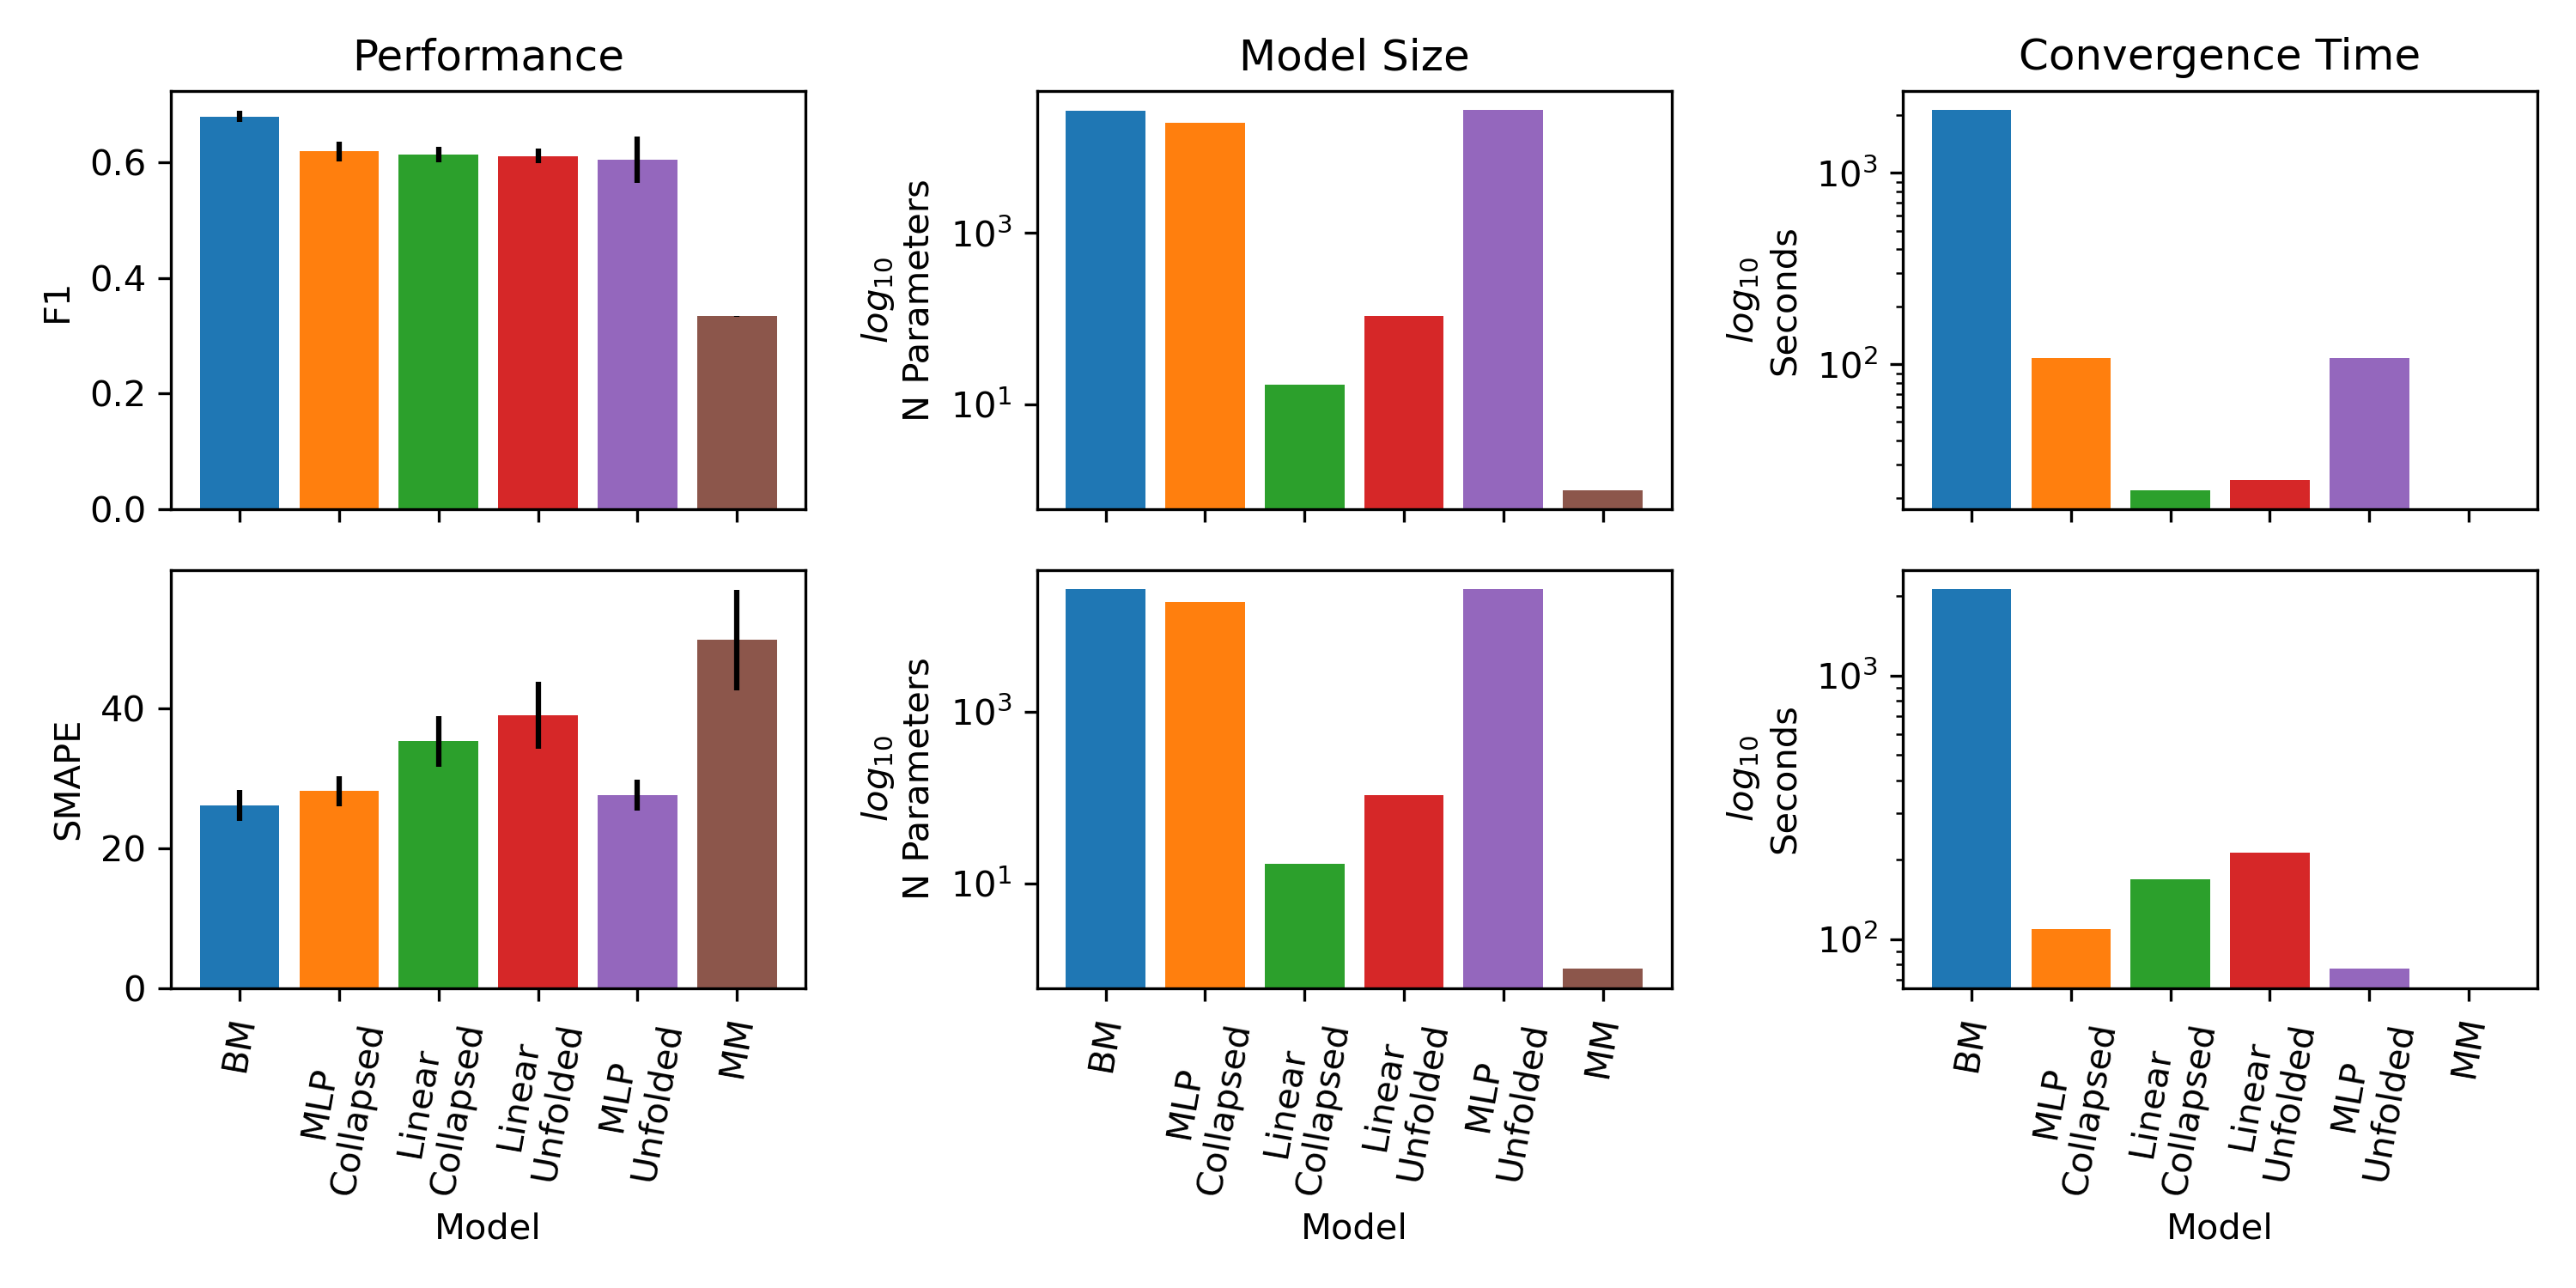
\includegraphics[width=.7\textwidth]{images/chapter_3/global_31.png}
\caption[\textbf{Aggregated comparison of models' performance}]{The BM architecture outperformed all competing ones on both target using however more parameters and computation time. Bar-plots in the first column show the average performance across the 6 game contexts along with estimated standard errors of the mean. The bar-plots on the second and third columns express the number of parameters and the convergence time for each model.}
\label{model_comp_coll_31} 
\end{figure*}
\begin{table}[h]\centering
\caption{\textbf{Performance Baseline Mean Model}}
\label{baseperformance}
\resizebox{0.5\textwidth}{!}{
\begin{tabular}{@{}llrr@{}}
\toprule
\textbf{Game}  &\textbf{Model}                 & \textbf{SMAPE}      & \textbf{F1}       \\ \midrule
\textbf{hmg}   &\multirow{2}{*}{}               & $0.767 \pm 0.001$   & $0.500 \pm 0.003$ \\
\textbf{hms}   &                                & $0.581 \pm 0.001$   & $0.507 \pm 0.003$ \\
\textbf{jc3}   &\multirow{2}{*}{\textbf{MM}}    & $0.632 \pm 0.003$   & $0.499 \pm 0.004$ \\
\textbf{jc4}   &                                & $0.366 \pm 0.002$   & $0.499 \pm 0.001$ \\
\textbf{lis}   &\multirow{2}{*}{\textit{}}      & $0.404 \pm 0.001$   & $0.500 \pm 0.003$ \\
\textbf{lisbf} &                                & $0.244 \pm 0.002$   & $0.500 \pm 0.005$ \\ \bottomrule
\end{tabular}
}
\end{table}

The results from the predictive task carried out using the collapsed dataset, Table \ref{collapsedperformance}, showed how all the 4 models strongly outperformed the MM baseline, Table \ref{baseperformance}, in all games, while also achieving an overall satisfying performance. Moreover we noticed how MLPr and MLPc markedly outperformed EN and LR in both churn probability and survival time prediction across all games.  

\begin{table}[h] \centering
\caption{\textbf{Performance Collapsed Format}}
\label{collapsedperformance}
\resizebox{0.5\textwidth}{!}{
\begin{tabular}{@{}llrlr@{}}
\toprule
\textbf{Game}  &\textbf{Model}                & \textbf{SMAPE}       &\textbf{Model}                & \textbf{F1}       \\ \midrule
\textbf{hmg}   &\multirow{2}{*}{}             & $51.3 \pm 4.3$    &\multirow{2}{*}{}             & $0.591 \pm 0.004$ \\
\textbf{hms}   &                              & $33.1 \pm 2.0$    &                              & $0.624 \pm 0.004$ \\
\textbf{jc3}   &\multirow{2}{*}{\textbf{EN}}  & $42.3 \pm 0.8$    &\multirow{2}{*}{\textbf{LR}}  & $0.601 \pm 0.004$ \\
\textbf{jc4}   &                              & $35.1 \pm 0.6$    &                              & $0.663 \pm 0.002$ \\
\textbf{lis}   &\multirow{2}{*}{}             & $28.7 \pm 0.4$    &\multirow{2}{*}{}             & $0.626 \pm 0.003$ \\
\textbf{lisbf} &                              & $23.9 \pm 0.3$    &                              & $0.591 \pm 0.003$ \\ \midrule

\textbf{hmg}   &\multirow{2}{*}{}             & $30.4 \pm 0.8$    &\multirow{2}{*}{}             & $0.660 \pm 0.006$ \\
\textbf{hms}   &                              & $24.1 \pm 0.7$    &                              & $0.670 \pm 0.006$ \\
\textbf{jc3}   &\multirow{2}{*}{\textbf{MLPr}}& $36.0 \pm 0.3$    &\multirow{2}{*}{\textbf{MLPc}}& $0.654 \pm 0.004$ \\
\textbf{jc4}   &                              & $33.4 \pm 0.2$    &                              & $0.678 \pm 0.004$ \\
\textbf{lis}   &\multirow{2}{*}{\textit{}}    & $25.6 \pm 0.3$    &\multirow{2}{*}{\textit{}}    & $0.664 \pm 0.003$ \\
\textbf{lisbf} &                              & $21.9 \pm 0.2$    &                              & $0.622 \pm 0.003$ \\ \bottomrule
\end{tabular}
}
\end{table}

Looking at the same modelling approaches on the unfolded version of the same dataset we can observed a similar pattern of results, see Table \ref{unfoldedperformance}, regarding baseline and inter-models comparisons. However, it was clear that using unfolded, temporal data lead to only small improvements over the aggregated data. This might be explained by the fact that the chosen modelling approaches are not explicitly designed for taking temporal structure into account, for example they have no explicit mechanics for temporal modelling such as those provided by a LSTM.

\begin{table}[h] \centering
\caption{\textbf{Performance Unfolded Format}}
\label{unfoldedperformance}
\resizebox{0.5\textwidth}{!}{
\begin{tabular}{@{}llrlr@{}}
\toprule
\textbf{Game}  &\textbf{Model}                 & \textbf{SMAPE}  &\textbf{Model}               & \textbf{F1}       \\ \midrule
\textbf{hmg}   &\multirow{2}{*}{}             & $54.5 \pm 2.4$ &\multirow{2}{*}{}             & $0.612 \pm 0.004$ \\
\textbf{hms}   &                              & $55.0 \pm 2.0$ &                              & $0.626 \pm 0.004$ \\
\textbf{jc3}   &\multirow{2}{*}{\textbf{EN}}  & $38.4 \pm 0.3$ &\multirow{2}{*}{\textbf{LR}}  & $0.607 \pm 0.003$ \\
\textbf{jc4}   &                              & $34.9 \pm 0.2$ &                              & $0.660 \pm 0.003$ \\
\textbf{lis}   &\multirow{2}{*}{}             & $30.2 \pm 0.1$ &\multirow{2}{*}{}             & $0.641 \pm 0.004$ \\
\textbf{lisbf} &                              & $23.5 \pm 0.2$ &                              & $0.578 \pm 0.003$ \\ \midrule
\textbf{hmg}   &\multirow{2}{*}{}             & $29.3 \pm 0.4$ &\multirow{2}{*}{}             & $0.683 \pm 0.005$ \\
\textbf{hms}   &                              & $22.6 \pm 0.4$ &                              & $0.682 \pm 0.004$ \\
\textbf{jc3}   &\multirow{2}{*}{\textbf{MLPr}}& $36.0 \pm 0.3$ &\multirow{2}{*}{\textbf{MLPc}}& $0.643 \pm 0.004$ \\
\textbf{jc4}   &                              & $33.1 \pm 0.2$ &                              & $0.681 \pm 0.003$ \\
\textbf{lis}   &\multirow{2}{*}{\textit{}}    & $25.6 \pm 0.2$ &\multirow{2}{*}{\textit{}}    & $0.673 \pm 0.005$ \\
\textbf{lisbf} &                              & $21.8 \pm 0.1$ &                              & $0.627 \pm 0.003$ \\ \bottomrule
\end{tabular}
}
\end{table}

Indeed, when evaluating the performance of the BM, Table \ref{bifurcatingperformance}, on the unfolded data we can see how the model achieves consistent improvements in both churn probability and survival time prediction in all game contexts compared to the previous best model (MLPr and MLPc). From a visual inspection of Figure \ref{perfsurv} 

\begin{figure}[h]
  \centering
  \includegraphics[width=0.7\textwidth]{images/chapter_3/performance_survival_31.pdf}
  \caption[\textbf{Performance of the BM on survival task}]{The scatter plot shows the relationship between the survival time prediction provided by the BM and the ground truth values. Since the relationship is evaluated on the $log$ of both variables, due to the presence extreme outliers in the ground truth, this acts as mostly as a qualitative complement to the more reliable SMAPE measure.}
  \label{perfsurv}
\end{figure}

we can see the presence of a positive linear relationship between estimated and ground truth survival time (indicative of accordance between the two), with a roughly even distribution of error along the entire range of values. In Table \ref{confusionmatrix} \begin{table}[h] \centering
\caption[\textbf{Performance of the BM on churn task}]{Here the diagonal shows the \% of correct predictions for each label across all games.}
\label{confusionmatrix}
\begin{tabular}{llcc}
\toprule
 & & \multicolumn{2}{c}{\textbf{Prediction}} \\ \cmidrule(lr){3-4}
 & & \parbox[c]{1.5cm}{Churner} & \parbox[c]{1.5cm}{Non-Churner} \\ \midrule
\multirow{2}{*}{\rotatebox{90}{\parbox[c]{1.5cm}{\textbf{Ground  Truth}}}} 
&\multirow{2}{*}{Churner}  & \cellcolor{DarkOliveGreen3!69}   &  \cellcolor{DarkOliveGreen3!31}   \\ 
&&\multirow{-2}{*}{\cellcolor{DarkOliveGreen3!69}0.69}& \multirow{-2}{*}{\cellcolor{DarkOliveGreen3!31}0.31}\\
&\multirow{2}{*}{Non-Churner}  &  \cellcolor{DarkOliveGreen3!33}   &  \cellcolor{DarkOliveGreen3!66}   \\ 
&  &  \multirow{-2}{*}{\cellcolor{DarkOliveGreen3!33} 0.33} & \multirow{-2}{*}{\cellcolor{DarkOliveGreen3!66} 0.66}\\
\bottomrule
\end{tabular}
\end{table} 
we can observe how the model performance is evenly split across the two classes highlighting similar levels of precision and recall. 

Finally, observing the density plots in Figure \ref{fig:densurv} and \ref{fig:denchurn} we can see how the model was able to encode different levels of uncertainty in the predicted values through different levels of posterior variance.

\begin{figure}[h]
  \centering
  \subfloat[Survival Predictions]{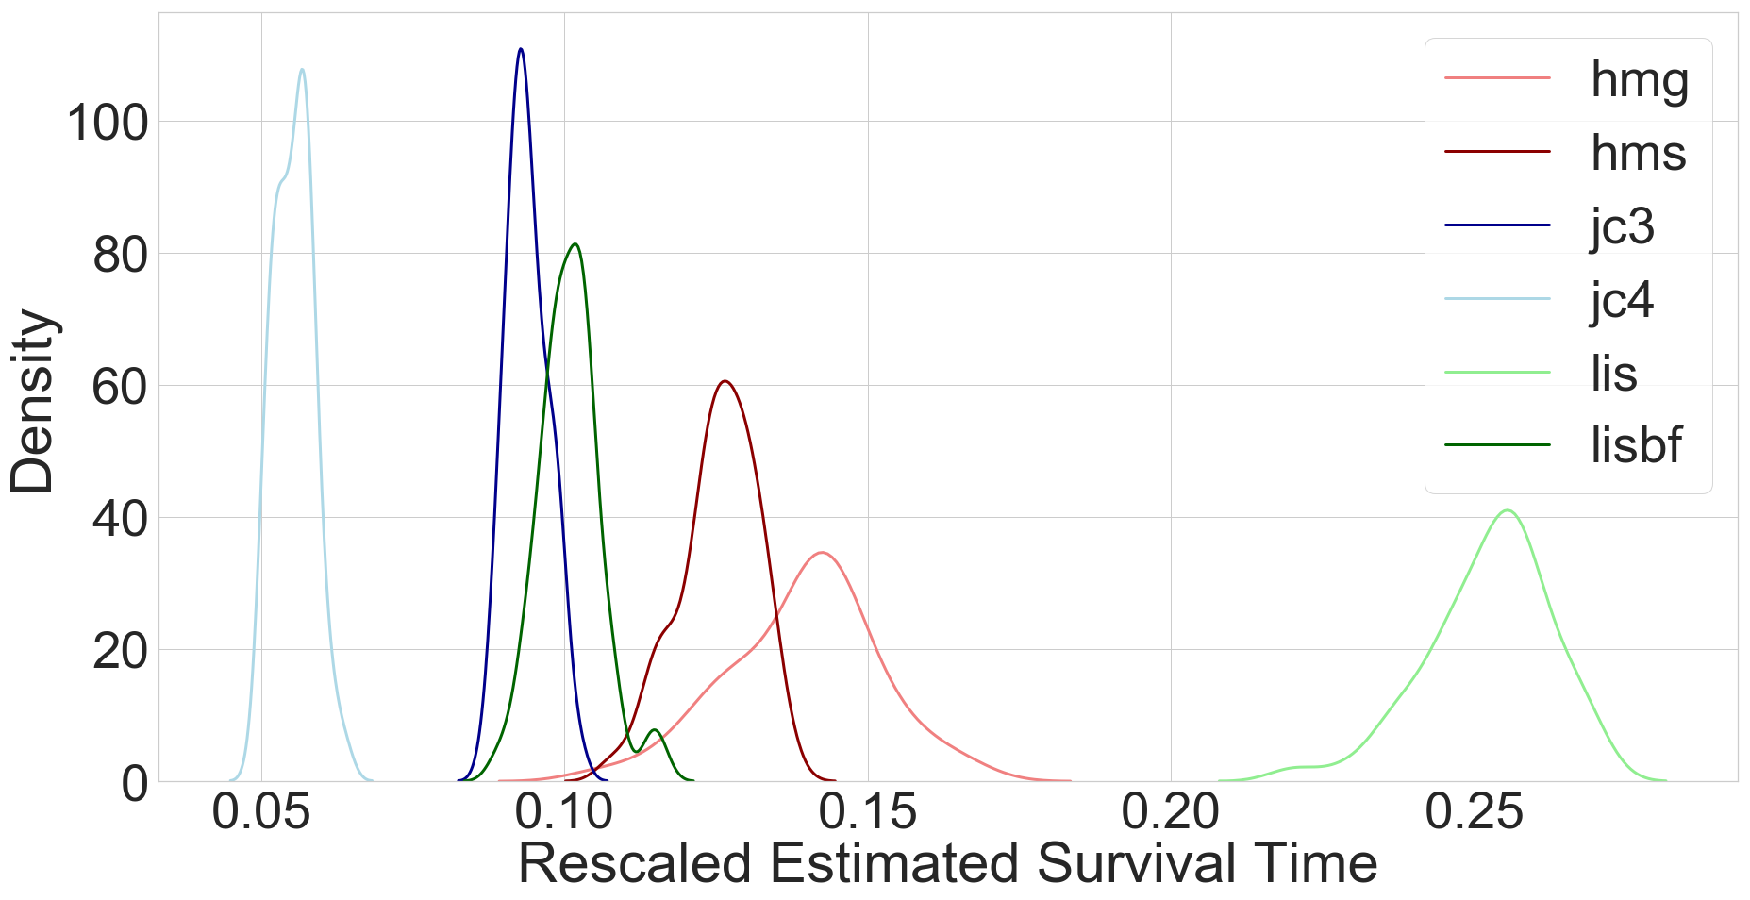
\includegraphics[ width=0.7\textwidth]{images/chapter_3/survival_density_31.pdf}\label{fig:densurv}}
  \hfill
  \subfloat[Churn Probability Predictions]{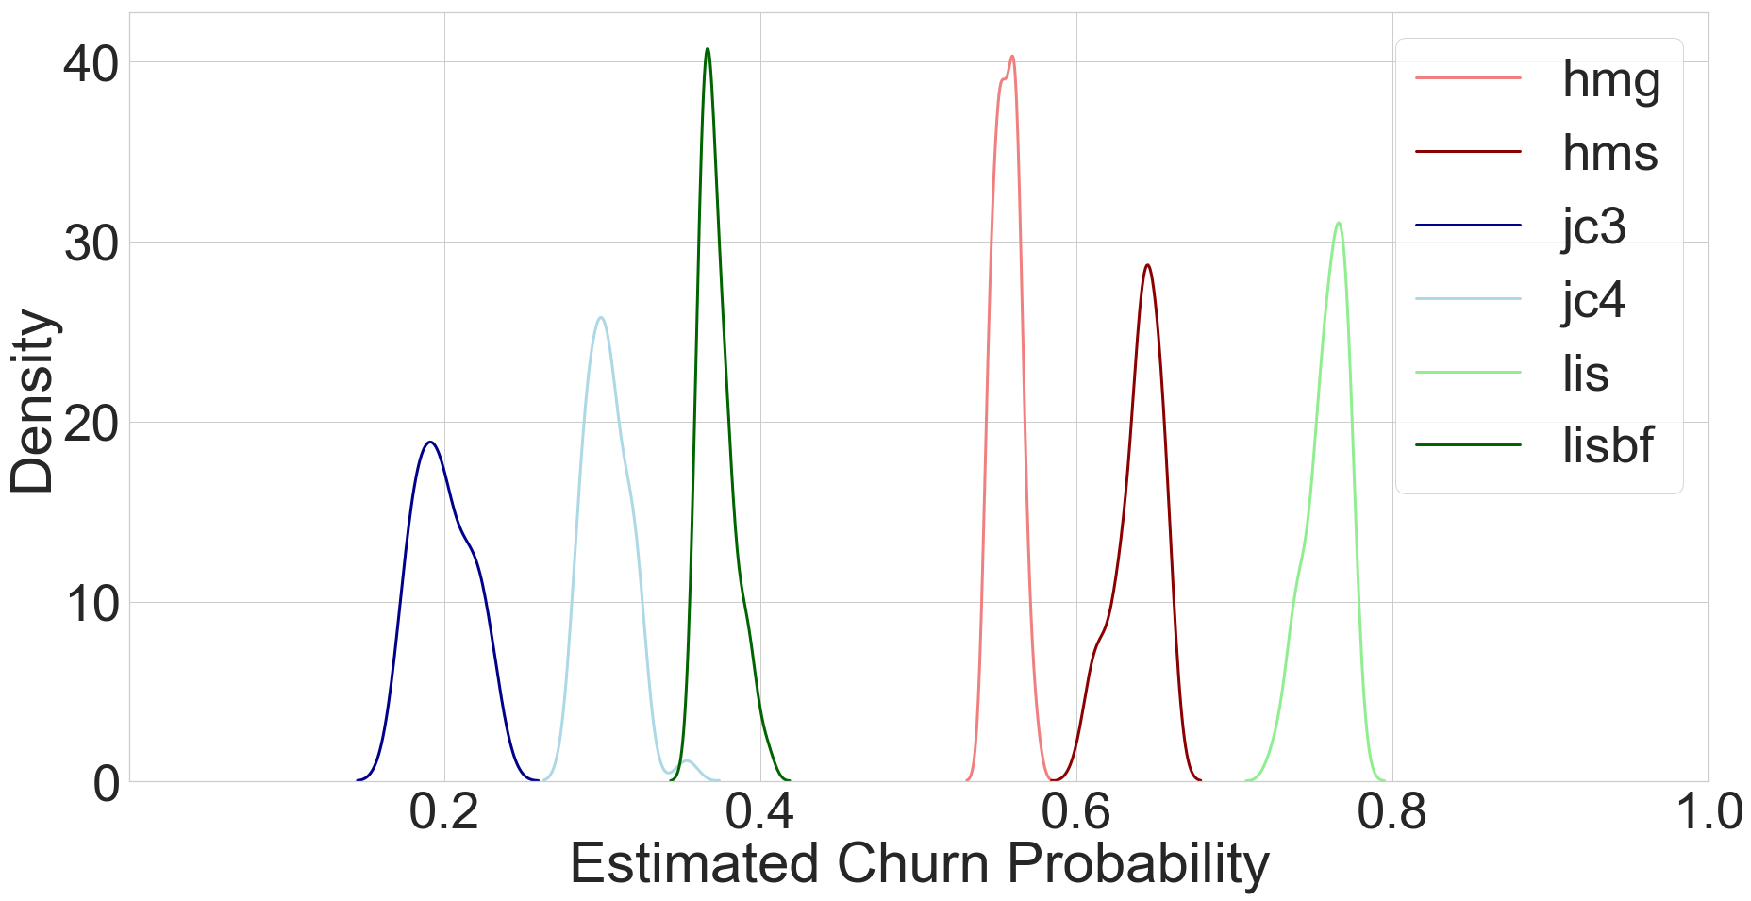
\includegraphics[ width=0.7\textwidth]{images/chapter_3/churn_density_31.pdf}\label{fig:denchurn}}
  \caption[\textbf{Distribution of the BM predictions for six random users, one for each game}]{For better comparison the survival estimates are re-scaled game-wise in the range 0 to 1. The highest density point in the distribution represents the most probable predicted value (i.e. the actual prediction),  while the area under the curve instead can be seen as measure of uncertainty (i.e. how confident is the model in its prediction).}
  \label{distestimations}
\end{figure}

\begin{table}[h] \centering
\caption{\textbf{Performance Bifurcating Model}}
\label{bifurcatingperformance}
\resizebox{0.5\textwidth}{!}{
\begin{tabular}{@{}llrr@{}}
\toprule
\textbf{Game}  &\textbf{Models}               & \textbf{SMAPE}      & \textbf{F1}       \\ \midrule
\textbf{hmg}   &\multirow{2}{*}{}             & $27.5 \pm 0.1$   & $0.693 \pm 0.002$ \\
\textbf{hms}   &                              & $20.0 \pm 0.1$   & $0.701 \pm 0.003$ \\
\textbf{jc3}   &\multirow{2}{*}{\textbf{BM}}  & $34.4 \pm 0.3$   & $0.671 \pm 0.005$ \\
\textbf{jc4}   &                              & $32.5 \pm 0.2$   & $0.685 \pm 0.002$ \\
\textbf{lis}   &\multirow{2}{*}{}             & $24.6 \pm 0.2$   & $0.688 \pm 0.003$ \\
\textbf{lisbf} &                              & $20.8 \pm 0.1$   & $0.645 \pm 0.003$ \\ \bottomrule
\end{tabular}
}
\end{table}

\subsection{Model Criticism}
\label{model_criticims_1}
The different level of performance achieved by the baseline model highlighted how different game context proved to be a more challenging ground (e.g. $jc4$ and $lisbf$) than others with respect to the predictive task. 

Although we did not perform an exhaustive test for evaluating if disjoint models (i.e. models fitted separately to each game context) would outperform our joint modelling approach, we noticed how each parametric model (which all adopt a joint modelling approach) outperformed the baseline(which adopts a disjoint modelling approach) while maintaining a similar performance distribution across game contexts. 

By looking at the performance of the various parametric models we saw how  the use of models able to capture non-linear interactions between features provided substantial improvements in predicting measures of future behavioural intensity. We also showed that considering the entire history of individual-game interactions provided a consistent but small edge over metrics representations which are collapsed over time. However, this improvement appeared to be markedly more pronounced and consistent when the predictive task was carried out by non-linear models able to take the dynamical nature of the data into account (e.g., the proposed BM architecture). Finally, by looking more in details at the performance of the the BM highlighted how the proposed methodology generalizes well when trying to predict survival time and churn probability as well as successfully incorporating measures of uncertainty in its estimations. 

In summary, the BM architecture designed following the theoretical principles outlined in chapter \ref{chapter_theory_modelling} showed improved predictive accuracy when compared to alternatives with comparable computational expressiveness (i.e., the MLP architectures). 

That said, it is evident that the architecture does not come fully equipped with all the constrains outlined in chapter \ref{chapter_theory_modelling}
which are necessary for obtaining a good approximation of the type of construct (i.e., attributed incentive salience) presented in the works of McClure et al. \cite{mcclure2003computational} and Zhang et al. \cite{zhang2009neural}. First of all the BM architecture aims at predicting the cumulative expected amount of future behaviour at an arbitrary early point in time $t \ll T$ (the OP defined in section \ref{model_design_1}). This implies that, despite the latent representation generated at time $t$ possesses similar predictive powers to attributed incentive salience, these are not on the same time scale and most importantly are not defined for all the $t \in T$. Secondly, despite churn probability and survival time can be considered good approximations of future behavioural intensity, they surely do not fully capture the complexity of the phenomenon. Moreover, these two metrics can be considered of second order (i.e., they are derived from raw quantifiers of behaviour intensity) and artificially created for serving specific concrete applications in the context of engagement quantification. 

Since the aim of this thesis is to estimate motivation related latent states (from which, as we said in chapter \ref{chapter_lit_review}, the behavioural manifestation of engagement can be directly derived) the next iteration in our model building process focused on modifying the BM architecture in order to make its functional form closer to what highlighted in chapter \ref{chapter_theory_modelling}.

\section{Dynamic Prediction of Future Behavioural Intensity}
\label{model_architecture_2}
In the second iteration of our model building process we focused on improving and expanding the BM architecture in order to increase its flexibility and ability to incorporate the functional constrains specified in chapter \ref{chapter_theory_modelling}. 

Two major constrains were introduced:
\begin{enumerate}
    \item The new architecture had to jointly predict 5 behavioural metrics. These, differently from churn and survival time, were first order indicator of future behavioural intensity similar to those find in the behavioural neuroscience literature \cite{schultz1997neural,mcclure2003computational,berridge2004motivation,zhang2009neural}
    
    \item We moved the predictive task from a "static" (i.e., predicting a long-term target after observing a fixed sequence of individual-game interaction) to a "dynamic" one (i.e., performing prediction after each new interaction is observed).
\end{enumerate}

In line with these constrains the experimental task used in this second stage of the model building process aimed at predicting the behavioural intensity of the next interaction between an individual and a videogame after observing an arbitrary number of interactions. More formally, given a sequence of interactions with associated behavioural intensity $B_{t_1 : T}$, the target of the model at any given point in time $t_n$ became
\begin{equation}
\label{joint_target_eq}
   B_{t_{n+1}} = \{b^1_{t_{n+1}}, \dots,  b^5_{t_{n+1}}\}
\end{equation}
with $\{b^1_{t_{n+1}}, \dots, b^5_{t_{n+1}}\}$ being the lead-1 version of the behavioural inputs provided to the model (more details are provided in sections \ref{model_design_2} and \ref{data_2}. This new task is now in line with the formulation presented in section \ref{td_to_supervised} and correspond to predicting the behavioural manifestations of all the phases of the engagement process model \cite{o2008user}, however in a dynamic fashion. 

The major aim of this second experimental task was to validate the results obtained during the evaluation of the BM architecture while submitting to model constrains that were consistent with the theoretical framework presented in chapter \ref{chapter_lit_review} and \ref{chapter_theory_modelling}. In this view, the hypotheses that we wanted to validate were tightly connected with those presented in section \ref{model_architecture_1}, and had the following form:
\begin{enumerate}
    \item Approaches able to account for non-linear interactions in the considered behavioural metrics can outperform simpler additive models.
    \item The ability to model the type of sequential dynamics presented in section \ref{td_to_supervised} can have a positive effect on the predictive performance.
    \item It is possible to have a single model jointly multiple first-order metrics of behavioural intensity without any substantial loss in accuracy
    \item It is possible to have a single model performing the predictive task simultaneously across a wide range of games.
\end{enumerate}

\subsection{Model Design}
\label{model_design_2}
The second iteration of our ANN architecture was a direct descendant of the BM architecture and aimed to jointly predict a set of 5 behavioural metrics all indicative of the intensity of interactions between an individual and a videogame. 

Despite being markedly different, our architecture shares similarities with technique used in the neuroscience literature for inferring latent states able to predict observable behaviours \cite{calhoun2019unsupervised}. For example Calhoun et al. used a combination of Hidden Markov Model (HMM) and Generalized Linear Model (GLM) for analyzing the natural behaviour of flies \cite{calhoun2019unsupervised}. Similarly to our proposed architecture, the HMM-GLM approach first infer a latent representation of the observed behaviour though a dynamical model (i.e., HMM) and then uses the same representation for performing predictions using a set of non-linear additive model (i.e., GLM). Our architecture, that we call recurrent (RNN) for simplicity, illustrated in Figure \ref{fig: rnn_2} extends the work of Calhoun et al. by removing the additive and markovian assumptions and by dropping the requirement for a fixed number of hidden states.

\begin{figure}[ht]
\begin{center}
\begin{adjustbox}{width=0.5\textwidth}

   \tikzset{every picture/.style={line width=0.75pt}} %set default line width to 0.75pt        

    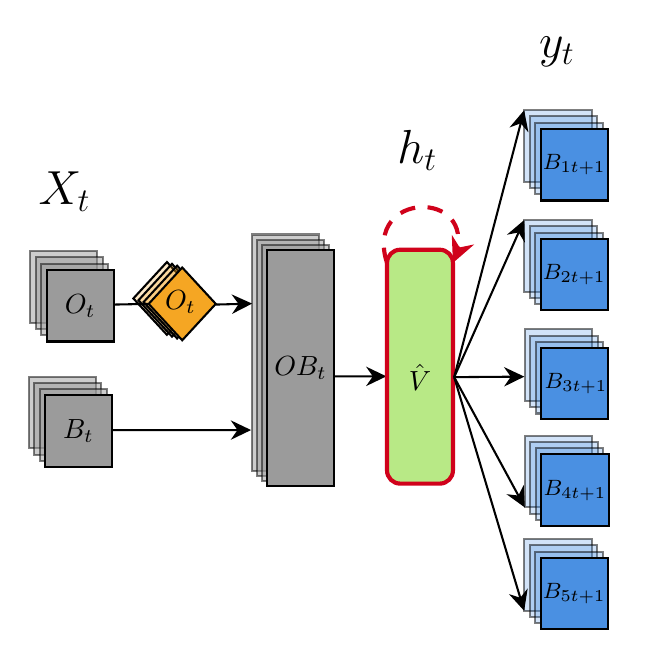
\begin{tikzpicture}[x=0.75pt,y=0.75pt,yscale=-1,xscale=1]
    %uncomment if require: \path (0,354); %set diagram left start at 0, and has height of 354
    
    %Shape: Diamond [id:dp7904557337929367] 
    \draw  [fill={rgb, 255:red, 245; green, 166; blue, 35 }  ,fill opacity=0.25 ] (251.6,119.28) -- (267.77,136.81) -- (251.6,154.33) -- (235.43,136.81) -- cycle ;
    %Shape: Diamond [id:dp44140375398321585] 
    \draw  [fill={rgb, 255:red, 245; green, 166; blue, 35 }  ,fill opacity=0.25 ] (254.05,120.16) -- (270.22,137.68) -- (254.05,155.2) -- (237.89,137.68) -- cycle ;
    %Shape: Diamond [id:dp3808148721846334] 
    \draw  [fill={rgb, 255:red, 245; green, 166; blue, 35 }  ,fill opacity=0.25 ] (256.51,121.04) -- (272.68,138.56) -- (256.51,156.08) -- (240.34,138.56) -- cycle ;
    %Shape: Rectangle [id:dp6212572558437682] 
    \draw  [color={rgb, 255:red, 0; green, 0; blue, 0 }  ,draw opacity=0.5 ][fill={rgb, 255:red, 155; green, 155; blue, 155 }  ,fill opacity=0.5 ] (292.41,106.01) -- (324.92,106.01) -- (324.92,219.74) -- (292.41,219.74) -- cycle ;
    %Shape: Rectangle [id:dp04308865519441296] 
    \draw  [color={rgb, 255:red, 0; green, 0; blue, 0 }  ,draw opacity=0.5 ][fill={rgb, 255:red, 155; green, 155; blue, 155 }  ,fill opacity=0.5 ] (294.86,108.47) -- (327.38,108.47) -- (327.38,222.2) -- (294.86,222.2) -- cycle ;
    %Shape: Rectangle [id:dp692301238884502] 
    \draw  [color={rgb, 255:red, 0; green, 0; blue, 0 }  ,draw opacity=0.5 ][fill={rgb, 255:red, 155; green, 155; blue, 155 }  ,fill opacity=0.5 ] (297.32,110.93) -- (329.84,110.93) -- (329.84,224.66) -- (297.32,224.66) -- cycle ;
    %Shape: Diamond [id:dp3746200743423901] 
    \draw  [fill={rgb, 255:red, 245; green, 166; blue, 35 }  ,fill opacity=1 ] (258.97,121.91) -- (275.13,139.43) -- (258.97,156.96) -- (242.8,139.43) -- cycle ;
    %Straight Lines [id:da9537882301539488] 
    \draw    (274.94,139.77) -- (289.65,139.38) ;
    \draw [shift={(292.65,139.3)}, rotate = 178.49] [fill={rgb, 255:red, 0; green, 0; blue, 0 }  ][line width=0.08]  [draw opacity=0] (9.82,-4.72) -- (0,0) -- (9.82,4.72) -- (6.52,0) -- cycle    ;
    %Straight Lines [id:da45479882207763933] 
    \draw [fill={rgb, 255:red, 155; green, 155; blue, 155 }  ,fill opacity=1 ]   (203.09,200.3) -- (289.13,200.22) ;
    \draw [shift={(292.13,200.22)}, rotate = 179.95] [fill={rgb, 255:red, 0; green, 0; blue, 0 }  ][line width=0.08]  [draw opacity=0] (9.82,-4.72) -- (0,0) -- (9.82,4.72) -- (6.52,0) -- cycle    ;
    %Straight Lines [id:da9952506139878592] 
    \draw [fill={rgb, 255:red, 155; green, 155; blue, 155 }  ,fill opacity=1 ]   (324.42,174.36) -- (354.33,174.35) ;
    \draw [shift={(357.33,174.35)}, rotate = 179.97] [fill={rgb, 255:red, 0; green, 0; blue, 0 }  ][line width=0.08]  [draw opacity=0] (9.82,-4.72) -- (0,0) -- (9.82,4.72) -- (6.52,0) -- cycle    ;
    %Shape: Rectangle [id:dp5105796971723443] 
    \draw  [color={rgb, 255:red, 0; green, 0; blue, 0 }  ,draw opacity=0.5 ][fill={rgb, 255:red, 155; green, 155; blue, 155 }  ,fill opacity=0.5 ] (185.01,174.53) -- (217.26,174.53) -- (217.26,209.05) -- (185.01,209.05) -- cycle ;
    %Shape: Rectangle [id:dp2595806858227925] 
    \draw  [color={rgb, 255:red, 0; green, 0; blue, 0 }  ,draw opacity=0.5 ][fill={rgb, 255:red, 155; green, 155; blue, 155 }  ,fill opacity=0.5 ] (187.63,177.51) -- (219.88,177.51) -- (219.88,212.03) -- (187.63,212.03) -- cycle ;
    %Shape: Rectangle [id:dp8277252726471348] 
    \draw  [color={rgb, 255:red, 0; green, 0; blue, 0 }  ,draw opacity=0.5 ][fill={rgb, 255:red, 155; green, 155; blue, 155 }  ,fill opacity=0.5 ] (190.27,180.56) -- (222.53,180.56) -- (222.53,215.08) -- (190.27,215.08) -- cycle ;
    %Shape: Rectangle [id:dp4311381435790056] 
    \draw  [fill={rgb, 255:red, 155; green, 155; blue, 155 }  ,fill opacity=1 ] (192.86,183.5) -- (225.11,183.5) -- (225.11,218.02) -- (192.86,218.02) -- cycle ;
    %Shape: Rectangle [id:dp5047118561624738] 
    \draw  [fill={rgb, 255:red, 155; green, 155; blue, 155 }  ,fill opacity=1 ] (299.77,113.39) -- (332.29,113.39) -- (332.29,227.12) -- (299.77,227.12) -- cycle ;
    %Shape: Rectangle [id:dp21573647855268596] 
    \draw  [color={rgb, 255:red, 0; green, 0; blue, 0 }  ,draw opacity=0.5 ][fill={rgb, 255:red, 155; green, 155; blue, 155 }  ,fill opacity=0.5 ] (185.83,114.08) -- (218.08,114.08) -- (218.08,148.6) -- (185.83,148.6) -- cycle ;
    %Shape: Rectangle [id:dp8439578107486148] 
    \draw  [color={rgb, 255:red, 0; green, 0; blue, 0 }  ,draw opacity=0.5 ][fill={rgb, 255:red, 155; green, 155; blue, 155 }  ,fill opacity=0.5 ] (188.45,117.06) -- (220.7,117.06) -- (220.7,151.58) -- (188.45,151.58) -- cycle ;
    %Shape: Rectangle [id:dp3660318943838672] 
    \draw  [color={rgb, 255:red, 0; green, 0; blue, 0 }  ,draw opacity=0.5 ][fill={rgb, 255:red, 155; green, 155; blue, 155 }  ,fill opacity=0.5 ] (191.09,120.11) -- (223.35,120.11) -- (223.35,154.63) -- (191.09,154.63) -- cycle ;
    %Shape: Rectangle [id:dp7778058544321894] 
    \draw  [fill={rgb, 255:red, 155; green, 155; blue, 155 }  ,fill opacity=1 ] (193.68,123.05) -- (225.93,123.05) -- (225.93,157.57) -- (193.68,157.57) -- cycle ;
    %Straight Lines [id:da7015539931476137] 
    \draw    (225.82,139.77) -- (242.8,139.43) ;
    %Rounded Rect [id:dp4473399888202214] 
    \draw  [color={rgb, 255:red, 208; green, 2; blue, 27 }  ,draw opacity=1 ][fill={rgb, 255:red, 184; green, 233; blue, 134 }  ,fill opacity=1 ][line width=1.5]  (357.64,119.69) .. controls (357.64,116.18) and (360.48,113.34) .. (363.99,113.34) -- (383.05,113.34) .. controls (386.56,113.34) and (389.4,116.18) .. (389.4,119.69) -- (389.4,219.68) .. controls (389.4,223.19) and (386.56,226.03) .. (383.05,226.03) -- (363.99,226.03) .. controls (360.48,226.03) and (357.64,223.19) .. (357.64,219.68) -- cycle ;
    %Curve Lines [id:da30430836514862303] 
    \draw [color={rgb, 255:red, 208; green, 2; blue, 27 }  ,draw opacity=1 ][line width=1.5]  [dash pattern={on 5.63pt off 4.5pt}]  (357.64,119.69) .. controls (346.28,85.07) and (400.82,83.85) .. (390.76,116.05) ;
    \draw [shift={(389.4,119.69)}, rotate = 293.32] [fill={rgb, 255:red, 208; green, 2; blue, 27 }  ,fill opacity=1 ][line width=0.08]  [draw opacity=0] (12.23,-5.88) -- (0,0) -- (12.23,5.88) -- (8.12,0) -- cycle    ;
    %Shape: Rectangle [id:dp9161667828288995] 
    \draw  [color={rgb, 255:red, 0; green, 0; blue, 0 }  ,draw opacity=0.5 ][fill={rgb, 255:red, 74; green, 144; blue, 226 }  ,fill opacity=0.25 ] (423.7,99.06) -- (456.2,99.06) -- (456.2,133.57) -- (423.7,133.57) -- cycle ;
    %Shape: Rectangle [id:dp20889912329934768] 
    \draw  [color={rgb, 255:red, 0; green, 0; blue, 0 }  ,draw opacity=0.5 ][fill={rgb, 255:red, 74; green, 144; blue, 226 }  ,fill opacity=0.25 ] (426.34,102.04) -- (458.84,102.04) -- (458.84,136.54) -- (426.34,136.54) -- cycle ;
    %Shape: Rectangle [id:dp2816776467625347] 
    \draw  [color={rgb, 255:red, 0; green, 0; blue, 0 }  ,draw opacity=0.5 ][fill={rgb, 255:red, 74; green, 144; blue, 226 }  ,fill opacity=0.25 ] (429,105.09) -- (461.51,105.09) -- (461.51,139.6) -- (429,139.6) -- cycle ;
    %Shape: Rectangle [id:dp42330781005921503] 
    \draw  [fill={rgb, 255:red, 74; green, 144; blue, 226 }  ,fill opacity=1 ] (431.61,108.03) -- (464.11,108.03) -- (464.11,142.53) -- (431.61,142.53) -- cycle ;
    %Shape: Rectangle [id:dp687693866282439] 
    \draw  [color={rgb, 255:red, 0; green, 0; blue, 0 }  ,draw opacity=0.5 ][fill={rgb, 255:red, 74; green, 144; blue, 226 }  ,fill opacity=0.25 ] (424.03,151.72) -- (456.53,151.72) -- (456.53,186.23) -- (424.03,186.23) -- cycle ;
    %Shape: Rectangle [id:dp48312027278133507] 
    \draw  [color={rgb, 255:red, 0; green, 0; blue, 0 }  ,draw opacity=0.5 ][fill={rgb, 255:red, 74; green, 144; blue, 226 }  ,fill opacity=0.25 ] (426.67,154.7) -- (459.17,154.7) -- (459.17,189.21) -- (426.67,189.21) -- cycle ;
    %Shape: Rectangle [id:dp5685283982245644] 
    \draw  [color={rgb, 255:red, 0; green, 0; blue, 0 }  ,draw opacity=0.5 ][fill={rgb, 255:red, 74; green, 144; blue, 226 }  ,fill opacity=0.25 ] (429.33,157.76) -- (461.84,157.76) -- (461.84,192.26) -- (429.33,192.26) -- cycle ;
    %Shape: Rectangle [id:dp3612684141121718] 
    \draw  [fill={rgb, 255:red, 74; green, 144; blue, 226 }  ,fill opacity=1 ] (431.95,160.69) -- (464.17,160.69) -- (464.17,194.89) -- (431.95,194.89) -- cycle ;
    %Shape: Rectangle [id:dp17418879327554693] 
    \draw  [color={rgb, 255:red, 0; green, 0; blue, 0 }  ,draw opacity=0.5 ][fill={rgb, 255:red, 74; green, 144; blue, 226 }  ,fill opacity=0.25 ] (423.7,252.78) -- (456.2,252.78) -- (456.2,287.29) -- (423.7,287.29) -- cycle ;
    %Shape: Rectangle [id:dp6752714184560265] 
    \draw  [color={rgb, 255:red, 0; green, 0; blue, 0 }  ,draw opacity=0.5 ][fill={rgb, 255:red, 74; green, 144; blue, 226 }  ,fill opacity=0.25 ] (426.34,255.76) -- (458.84,255.76) -- (458.84,290.26) -- (426.34,290.26) -- cycle ;
    %Shape: Rectangle [id:dp9983191940012098] 
    \draw  [color={rgb, 255:red, 0; green, 0; blue, 0 }  ,draw opacity=0.5 ][fill={rgb, 255:red, 74; green, 144; blue, 226 }  ,fill opacity=0.25 ] (429,258.81) -- (461.51,258.81) -- (461.51,293.32) -- (429,293.32) -- cycle ;
    %Shape: Rectangle [id:dp11003700320217247] 
    \draw  [fill={rgb, 255:red, 74; green, 144; blue, 226 }  ,fill opacity=1 ] (431.61,261.75) -- (464.11,261.75) -- (464.11,296.25) -- (431.61,296.25) -- cycle ;
    %Shape: Rectangle [id:dp7367493878137299] 
    \draw  [color={rgb, 255:red, 0; green, 0; blue, 0 }  ,draw opacity=0.5 ][fill={rgb, 255:red, 74; green, 144; blue, 226 }  ,fill opacity=0.25 ] (424.03,202.99) -- (456.53,202.99) -- (456.53,237.5) -- (424.03,237.5) -- cycle ;
    %Shape: Rectangle [id:dp8983348276713422] 
    \draw  [color={rgb, 255:red, 0; green, 0; blue, 0 }  ,draw opacity=0.5 ][fill={rgb, 255:red, 74; green, 144; blue, 226 }  ,fill opacity=0.25 ] (426.67,205.97) -- (459.17,205.97) -- (459.17,240.47) -- (426.67,240.47) -- cycle ;
    %Shape: Rectangle [id:dp09933660328753013] 
    \draw  [color={rgb, 255:red, 0; green, 0; blue, 0 }  ,draw opacity=0.5 ][fill={rgb, 255:red, 74; green, 144; blue, 226 }  ,fill opacity=0.25 ] (429.33,209.02) -- (461.84,209.02) -- (461.84,243.53) -- (429.33,243.53) -- cycle ;
    %Shape: Rectangle [id:dp9943795167198757] 
    \draw  [fill={rgb, 255:red, 74; green, 144; blue, 226 }  ,fill opacity=1 ] (431.94,211.96) -- (464.44,211.96) -- (464.44,246.46) -- (431.94,246.46) -- cycle ;
    %Shape: Rectangle [id:dp058820430549127] 
    \draw  [color={rgb, 255:red, 0; green, 0; blue, 0 }  ,draw opacity=0.5 ][fill={rgb, 255:red, 74; green, 144; blue, 226 }  ,fill opacity=0.25 ] (423.7,46.14) -- (456.2,46.14) -- (456.2,80.65) -- (423.7,80.65) -- cycle ;
    %Shape: Rectangle [id:dp9593581977954196] 
    \draw  [color={rgb, 255:red, 0; green, 0; blue, 0 }  ,draw opacity=0.5 ][fill={rgb, 255:red, 74; green, 144; blue, 226 }  ,fill opacity=0.25 ] (426.34,49.12) -- (458.84,49.12) -- (458.84,83.63) -- (426.34,83.63) -- cycle ;
    %Shape: Rectangle [id:dp4362593009406618] 
    \draw  [color={rgb, 255:red, 0; green, 0; blue, 0 }  ,draw opacity=0.5 ][fill={rgb, 255:red, 74; green, 144; blue, 226 }  ,fill opacity=0.25 ] (429,52.17) -- (461.51,52.17) -- (461.51,86.68) -- (429,86.68) -- cycle ;
    %Shape: Rectangle [id:dp7619519997532663] 
    \draw  [fill={rgb, 255:red, 74; green, 144; blue, 226 }  ,fill opacity=1 ] (431.61,55.11) -- (464.11,55.11) -- (464.11,89.62) -- (431.61,89.62) -- cycle ;
    %Straight Lines [id:da545267197618029] 
    \draw    (390,174.73) -- (422.94,49.05) ;
    \draw [shift={(423.7,46.14)}, rotate = 104.68] [fill={rgb, 255:red, 0; green, 0; blue, 0 }  ][line width=0.08]  [draw opacity=0] (9.82,-4.72) -- (0,0) -- (9.82,4.72) -- (6.52,0) -- cycle    ;
    %Straight Lines [id:da9271821433537066] 
    \draw    (390,174.73) -- (422.48,101.8) ;
    \draw [shift={(423.7,99.06)}, rotate = 114] [fill={rgb, 255:red, 0; green, 0; blue, 0 }  ][line width=0.08]  [draw opacity=0] (9.82,-4.72) -- (0,0) -- (9.82,4.72) -- (6.52,0) -- cycle    ;
    %Straight Lines [id:da6232303168074279] 
    \draw    (390,174.73) -- (420.8,174.5) ;
    \draw [shift={(423.8,174.48)}, rotate = 179.57] [fill={rgb, 255:red, 0; green, 0; blue, 0 }  ][line width=0.08]  [draw opacity=0] (9.82,-4.72) -- (0,0) -- (9.82,4.72) -- (6.52,0) -- cycle    ;
    %Straight Lines [id:da1424758683168187] 
    \draw    (390,174.73) -- (422.6,234.86) ;
    \draw [shift={(424.03,237.5)}, rotate = 241.54] [fill={rgb, 255:red, 0; green, 0; blue, 0 }  ][line width=0.08]  [draw opacity=0] (9.82,-4.72) -- (0,0) -- (9.82,4.72) -- (6.52,0) -- cycle    ;
    %Straight Lines [id:da40105840572004403] 
    \draw    (390,174.73) -- (422.84,284.41) ;
    \draw [shift={(423.7,287.29)}, rotate = 253.33] [fill={rgb, 255:red, 0; green, 0; blue, 0 }  ][line width=0.08]  [draw opacity=0] (9.82,-4.72) -- (0,0) -- (9.82,4.72) -- (6.52,0) -- cycle    ;
    
    % Text Node
    \draw (208.99,200.76) node  [font=\normalsize]  {$B_{t}$};
    % Text Node
    \draw (373.52,174.8) node  [font=\normalsize]  {$\hat{V}$};
    % Text Node
    \draw (258.15,138.56) node  [font=\normalsize]  {$O_{t}$};
    % Text Node
    \draw (202.34,85.25) node  [font=\LARGE]  {$X_{t}$};
    % Text Node
    \draw (316.03,170.25) node  [font=\normalsize]  {$OB_{t}$};
    % Text Node
    \draw (209.81,140.31) node  [font=\normalsize]  {$O_{t}$};
    % Text Node
    \draw (372.34,65.6) node  [font=\LARGE]  {$h_{t}$};
    % Text Node
    \draw (447.86,125.28) node  [font=\footnotesize]  {$B_{2t+1}$};
    % Text Node
    \draw (448.74,177.94) node  [font=\footnotesize]  {$B_{3t+1}$};
    % Text Node
    \draw (448.19,229.21) node  [font=\footnotesize]  {$B_{4t+1}$};
    % Text Node
    \draw (447.86,279) node  [font=\footnotesize]  {$B_{5t+1}$};
    % Text Node
    \draw (439.54,18) node  [font=\LARGE]  {$y_{t}$};
    % Text Node
    \draw (447.86,72.36) node  [font=\footnotesize]  {$B_{1t+1}$};
    
    
    \end{tikzpicture}


\end{adjustbox}
\end{center}
\caption[\textbf{The recurrent architecture}]{Blue, orange and green shapes represent respectively feedforward, embedding and LSTM operations. Gray shapes indicate operations with no learnable parameters, such as tensor instantiation and concatenation. Stacked, transparent colouring indicates tensors with a sequential structure. Straight and curved arrows refer to the presence of feed-forward or recurrent information flow. The red highlight shows the portion of the model we hypothesize is inferring an approximation of attributed incentive salience.}
\label{fig: rnn_2}
\end{figure}

The model receives the same input of the architecture described in section \ref{model_design_2} with the major difference that no padding was required. Indeed we decided to exploit the ability of RNN to flexibly fit variable-length time series and opted for a data generator approach \footnote{See \cite{chollet2015keras,tensorflow2015-whitepaper} for implementation details.}, feeding data to the models in random batches with constant length within a batch. 

The type of operations performed by the architecture were identical to those presented in section \ref{model_design_1} although with 2 major differences. First, the recurrent component of the architecture was now of type many-to-many therefore producing an $H \in \mathbb{R}^{N \times T \times h}$ tensor constituting the sequence of hidden states produced by the LSTM operation after observing each element of the input time series\cite{bengio2017deep}. Second, the final step of the architecture now exploits the temporal nature of the latent representation generated by the RNN for predicting not just a single value but a sequence of values, namely the lead-1 version of the input time series. This was again achieved by means of multi-task learning with five ANNs with fully connected operations. 

In order to apply the fully connected operations to a sequence of latent states we distributed their computations across time \footnote{See \cite{chollet2015keras} for implementation details} (see Appendix \ref{time_distributed}) so that each ANN could produce a tensor of shape $\hat{y} \in \mathbb{R}^{N \times T \times 1}$. 

We want to highlight that the model now fully reflect the formulation presented in section \ref{td_to_supervised}, indeed if again we look at the representations generated by the LSTM in terms of expectation

\begin{gather}
\label{rnn_1_exp}
   h_t = f^1(O, B_{t}, h_{t-1}; \theta^1)  \\ \nonumber
   \mathbb{E}[B_{t+1}] = f^2(h_t; \theta^2) \\ \nonumber    
\end{gather}

we can can see how at each point in time the generated representation $h_t$ is mostly indicative of the behavioural intensity a time $t+1$ but it also needs to retain some predictive power for all the subsequent time steps. 

The model used a combination of $ReLU$, $ELU$ and $LReLU$ (see Appendix \ref{elu} and \ref{lelu}) as activations functions for the hidden units (more details on their selection are specified in \ref{tuning_comparison_2} whereas the link function used for generating the prediction was always the $identity$ function. As a regularization strategy we decided to drop the use of batch normalization, as it proved challenging to adopt with a multivariate time-series target, and introduces a variant of dropout (i.e., One Dimensional Spatial Dropout see Appendix \ref{spatial_dropout}) more suitable for time series data and applied it after each layer in the architecture.

\paragraph{Competing Models}
\label{competing_models_2}
As in the previous stage of the model building process a series of competing models were implemented for testing our hypotheses. 

First, we decided to improve our baseline by establishing two reasonable single-parameter models. The first is a Lag 1 model producing predictions according to the following rule:

\begin{equation}
   \begin{gathered}  
     B_{t+1} = B_{t}
     \label{lag_1}
  \end{gathered}
\end{equation}
here $t$ represent a single game session in a sequence of $T$ observed interactions while $B$ are the same behavioural metrics the RNN model receives as input (they are thoroughly described in section \ref{data_2}). The second is a Median model computing the expectation of each of the 5 targets according to the formula:

\begin{equation}
  \begin{gathered}  
    \overline{B_{t+1}} = \frac
      {\sum_{i=1}^{t+1} wB_{i}}
      {\sum_{i=1}^{t+1} w }\\
    B_{t+1} = median(\overline{B_{t+1}}) 
    \label{median}
  \end{gathered}
\end{equation}

here $\overline{B_{t+1}}$ is an exponentially weighted average of all the $B_t$ up to $t+1$ observed when fitting the model. This is computed separately for every individual in the dataset and the median value of each of the 5 targets is used a a constant prediction. These apparently naive models provide a surprisingly robust prediction baseline for time series that are not white noise \cite{hyndman2018forecasting} other than having a nice interpretation in terms of behavioural momentum \cite{nevin2000behavioral}: in conditions of high experienced reward the behaviour of an individual tends to be consistent over time (i.e. resistant to change). 

Similarly to the model used in the assessment of the BM architecture, a multi-task linear model with Elastic-Net regularization (ENet) \cite{zou2005regularization} was used to evaluate the performance of simple additive models. While for testing the effect of non linearity, a multi-task Multilayer Perceptron (MLP) was employed. Both model used an embedding operation for encoding information from the game context but the ENet model had the number of hidden units fixed to 1 an relied on an $identity$ activation function. This was done for avoiding to introduce non-linearity in the ENet model. Figure \ref{fig: mlp_2} show the architecture used for both the ENet and MLP models. We can see that differently from the models used in section \ref{model_architecture_1} the only difference with RNN architecture lies in the use of time distributed fully connected operations instead of those provided by the LSTM. 
\begin{figure}[ht]
\begin{center}
\begin{adjustbox}{width=0.7\textwidth}

\tikzset{every picture/.style={line width=0.75pt}} %set default line width to 0.75pt        

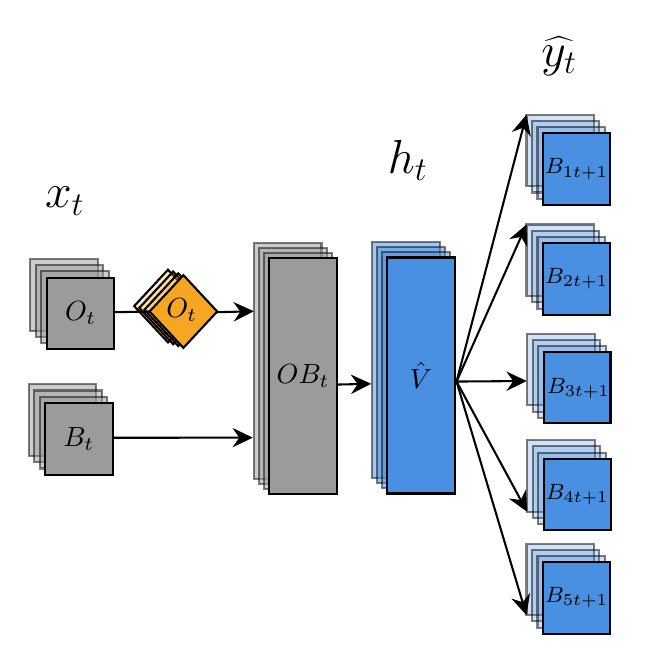
\begin{tikzpicture}[x=0.75pt,y=0.75pt,yscale=-1,xscale=1]
%uncomment if require: \path (0,331); %set diagram left start at 0, and has height of 331

%Shape: Diamond [id:dp8512741780313259] 
\draw  [fill={rgb, 255:red, 245; green, 166; blue, 35 }  ,fill opacity=0.25 ] (257.97,138.57) -- (274.27,156.09) -- (257.97,173.6) -- (241.68,156.09) -- cycle ;
%Shape: Diamond [id:dp44131568061643844] 
\draw  [fill={rgb, 255:red, 245; green, 166; blue, 35 }  ,fill opacity=0.25 ] (260.45,139.45) -- (276.74,156.96) -- (260.45,174.48) -- (244.15,156.96) -- cycle ;
%Shape: Diamond [id:dp9944377463655836] 
\draw  [fill={rgb, 255:red, 245; green, 166; blue, 35 }  ,fill opacity=0.25 ] (262.92,140.32) -- (279.22,157.84) -- (262.92,175.35) -- (246.63,157.84) -- cycle ;
%Shape: Rectangle [id:dp3605470636117536] 
\draw  [color={rgb, 255:red, 0; green, 0; blue, 0 }  ,draw opacity=0.5 ][fill={rgb, 255:red, 74; green, 144; blue, 226 }  ,fill opacity=0.5 ] (356.1,125.3) -- (388.87,125.3) -- (388.87,239) -- (356.1,239) -- cycle ;
%Shape: Rectangle [id:dp7194333726509892] 
\draw  [color={rgb, 255:red, 0; green, 0; blue, 0 }  ,draw opacity=0.5 ][fill={rgb, 255:red, 74; green, 144; blue, 226 }  ,fill opacity=0.5 ] (358.57,127.76) -- (391.34,127.76) -- (391.34,241.46) -- (358.57,241.46) -- cycle ;
%Shape: Rectangle [id:dp3276084138933598] 
\draw  [color={rgb, 255:red, 0; green, 0; blue, 0 }  ,draw opacity=0.5 ][fill={rgb, 255:red, 74; green, 144; blue, 226 }  ,fill opacity=0.5 ] (361.05,130.22) -- (393.82,130.22) -- (393.82,243.92) -- (361.05,243.92) -- cycle ;
%Shape: Diamond [id:dp6965315978812838] 
\draw  [fill={rgb, 255:red, 245; green, 166; blue, 35 }  ,fill opacity=1 ] (265.4,141.2) -- (281.69,158.71) -- (265.4,176.23) -- (249.1,158.71) -- cycle ;
%Straight Lines [id:da5408632178702979] 
\draw    (281.5,159.05) -- (296.35,158.66) ;
\draw [shift={(299.35,158.58)}, rotate = 178.5] [fill={rgb, 255:red, 0; green, 0; blue, 0 }  ][line width=0.08]  [draw opacity=0] (9.82,-4.72) -- (0,0) -- (9.82,4.72) -- (6.52,0) -- cycle    ;
%Straight Lines [id:da38550305545794683] 
\draw [fill={rgb, 255:red, 155; green, 155; blue, 155 }  ,fill opacity=1 ]   (209.09,219.56) -- (295.82,219.48) ;
\draw [shift={(298.82,219.48)}, rotate = 179.95] [fill={rgb, 255:red, 0; green, 0; blue, 0 }  ][line width=0.08]  [draw opacity=0] (9.82,-4.72) -- (0,0) -- (9.82,4.72) -- (6.52,0) -- cycle    ;
%Shape: Rectangle [id:dp8586026364143547] 
\draw  [color={rgb, 255:red, 0; green, 0; blue, 0 }  ,draw opacity=0.5 ][fill={rgb, 255:red, 74; green, 144; blue, 226 }  ,fill opacity=0.25 ] (430.7,116.78) -- (463.2,116.78) -- (463.2,151.29) -- (430.7,151.29) -- cycle ;
%Shape: Rectangle [id:dp5271658440371366] 
\draw  [color={rgb, 255:red, 0; green, 0; blue, 0 }  ,draw opacity=0.5 ][fill={rgb, 255:red, 74; green, 144; blue, 226 }  ,fill opacity=0.25 ] (433.34,119.76) -- (465.84,119.76) -- (465.84,154.27) -- (433.34,154.27) -- cycle ;
%Shape: Rectangle [id:dp6121896210605144] 
\draw  [color={rgb, 255:red, 0; green, 0; blue, 0 }  ,draw opacity=0.5 ][fill={rgb, 255:red, 74; green, 144; blue, 226 }  ,fill opacity=0.25 ] (436,122.81) -- (468.51,122.81) -- (468.51,157.32) -- (436,157.32) -- cycle ;
%Shape: Rectangle [id:dp2571940122217342] 
\draw  [fill={rgb, 255:red, 74; green, 144; blue, 226 }  ,fill opacity=1 ] (438.61,125.75) -- (471.11,125.75) -- (471.11,160.25) -- (438.61,160.25) -- cycle ;
%Shape: Rectangle [id:dp04921858860159267] 
\draw  [color={rgb, 255:red, 0; green, 0; blue, 0 }  ,draw opacity=0.5 ][fill={rgb, 255:red, 74; green, 144; blue, 226 }  ,fill opacity=0.25 ] (431.03,169.45) -- (463.53,169.45) -- (463.53,203.95) -- (431.03,203.95) -- cycle ;
%Shape: Rectangle [id:dp5512084563866699] 
\draw  [color={rgb, 255:red, 0; green, 0; blue, 0 }  ,draw opacity=0.5 ][fill={rgb, 255:red, 74; green, 144; blue, 226 }  ,fill opacity=0.25 ] (433.67,172.43) -- (466.17,172.43) -- (466.17,206.93) -- (433.67,206.93) -- cycle ;
%Shape: Rectangle [id:dp948946889597384] 
\draw  [color={rgb, 255:red, 0; green, 0; blue, 0 }  ,draw opacity=0.5 ][fill={rgb, 255:red, 74; green, 144; blue, 226 }  ,fill opacity=0.25 ] (436.33,175.48) -- (468.84,175.48) -- (468.84,209.98) -- (436.33,209.98) -- cycle ;
%Shape: Rectangle [id:dp7446725750615967] 
\draw  [fill={rgb, 255:red, 74; green, 144; blue, 226 }  ,fill opacity=1 ] (438.95,178.41) -- (471.17,178.41) -- (471.17,212.61) -- (438.95,212.61) -- cycle ;
%Shape: Rectangle [id:dp2953756097578333] 
\draw  [color={rgb, 255:red, 0; green, 0; blue, 0 }  ,draw opacity=0.5 ][fill={rgb, 255:red, 74; green, 144; blue, 226 }  ,fill opacity=0.25 ] (430.7,270.5) -- (463.2,270.5) -- (463.2,305.01) -- (430.7,305.01) -- cycle ;
%Shape: Rectangle [id:dp8190984811103563] 
\draw  [color={rgb, 255:red, 0; green, 0; blue, 0 }  ,draw opacity=0.5 ][fill={rgb, 255:red, 74; green, 144; blue, 226 }  ,fill opacity=0.25 ] (433.34,273.48) -- (465.84,273.48) -- (465.84,307.99) -- (433.34,307.99) -- cycle ;
%Shape: Rectangle [id:dp1989563986467071] 
\draw  [color={rgb, 255:red, 0; green, 0; blue, 0 }  ,draw opacity=0.5 ][fill={rgb, 255:red, 74; green, 144; blue, 226 }  ,fill opacity=0.25 ] (436,276.53) -- (468.51,276.53) -- (468.51,311.04) -- (436,311.04) -- cycle ;
%Shape: Rectangle [id:dp1924397511107222] 
\draw  [fill={rgb, 255:red, 74; green, 144; blue, 226 }  ,fill opacity=1 ] (438.61,279.47) -- (471.11,279.47) -- (471.11,313.98) -- (438.61,313.98) -- cycle ;
%Shape: Rectangle [id:dp8187051960536611] 
\draw  [color={rgb, 255:red, 0; green, 0; blue, 0 }  ,draw opacity=0.5 ][fill={rgb, 255:red, 74; green, 144; blue, 226 }  ,fill opacity=0.25 ] (431.03,220.71) -- (463.53,220.71) -- (463.53,255.22) -- (431.03,255.22) -- cycle ;
%Shape: Rectangle [id:dp6023578581008111] 
\draw  [color={rgb, 255:red, 0; green, 0; blue, 0 }  ,draw opacity=0.5 ][fill={rgb, 255:red, 74; green, 144; blue, 226 }  ,fill opacity=0.25 ] (433.67,223.69) -- (466.17,223.69) -- (466.17,258.2) -- (433.67,258.2) -- cycle ;
%Shape: Rectangle [id:dp8798703561171738] 
\draw  [color={rgb, 255:red, 0; green, 0; blue, 0 }  ,draw opacity=0.5 ][fill={rgb, 255:red, 74; green, 144; blue, 226 }  ,fill opacity=0.25 ] (436.33,226.74) -- (468.84,226.74) -- (468.84,261.25) -- (436.33,261.25) -- cycle ;
%Shape: Rectangle [id:dp3283044450373016] 
\draw  [fill={rgb, 255:red, 74; green, 144; blue, 226 }  ,fill opacity=1 ] (438.94,229.68) -- (471.44,229.68) -- (471.44,264.19) -- (438.94,264.19) -- cycle ;
%Shape: Rectangle [id:dp15154204076473643] 
\draw  [color={rgb, 255:red, 0; green, 0; blue, 0 }  ,draw opacity=0.5 ][fill={rgb, 255:red, 155; green, 155; blue, 155 }  ,fill opacity=0.5 ] (190.87,193.8) -- (223.37,193.8) -- (223.37,228.31) -- (190.87,228.31) -- cycle ;
%Shape: Rectangle [id:dp9182207029607203] 
\draw  [color={rgb, 255:red, 0; green, 0; blue, 0 }  ,draw opacity=0.5 ][fill={rgb, 255:red, 155; green, 155; blue, 155 }  ,fill opacity=0.5 ] (193.51,196.78) -- (226.01,196.78) -- (226.01,231.28) -- (193.51,231.28) -- cycle ;
%Shape: Rectangle [id:dp7698171692832448] 
\draw  [color={rgb, 255:red, 0; green, 0; blue, 0 }  ,draw opacity=0.5 ][fill={rgb, 255:red, 155; green, 155; blue, 155 }  ,fill opacity=0.5 ] (196.17,199.83) -- (228.68,199.83) -- (228.68,234.34) -- (196.17,234.34) -- cycle ;
%Shape: Rectangle [id:dp3865383455450443] 
\draw  [fill={rgb, 255:red, 155; green, 155; blue, 155 }  ,fill opacity=1 ] (198.78,202.77) -- (231.28,202.77) -- (231.28,237.27) -- (198.78,237.27) -- cycle ;
%Shape: Rectangle [id:dp23172130161456372] 
\draw  [fill={rgb, 255:red, 74; green, 144; blue, 226 }  ,fill opacity=1 ] (363.52,132.67) -- (396.29,132.67) -- (396.29,246.37) -- (363.52,246.37) -- cycle ;
%Shape: Rectangle [id:dp18125329077839125] 
\draw  [color={rgb, 255:red, 0; green, 0; blue, 0 }  ,draw opacity=0.5 ][fill={rgb, 255:red, 74; green, 144; blue, 226 }  ,fill opacity=0.25 ] (430.7,63.87) -- (463.2,63.87) -- (463.2,98.37) -- (430.7,98.37) -- cycle ;
%Shape: Rectangle [id:dp3729389269249752] 
\draw  [color={rgb, 255:red, 0; green, 0; blue, 0 }  ,draw opacity=0.5 ][fill={rgb, 255:red, 74; green, 144; blue, 226 }  ,fill opacity=0.25 ] (433.34,66.84) -- (465.84,66.84) -- (465.84,101.35) -- (433.34,101.35) -- cycle ;
%Shape: Rectangle [id:dp8889532693849542] 
\draw  [color={rgb, 255:red, 0; green, 0; blue, 0 }  ,draw opacity=0.5 ][fill={rgb, 255:red, 74; green, 144; blue, 226 }  ,fill opacity=0.25 ] (436,69.9) -- (468.51,69.9) -- (468.51,104.4) -- (436,104.4) -- cycle ;
%Shape: Rectangle [id:dp22768677359456946] 
\draw  [fill={rgb, 255:red, 74; green, 144; blue, 226 }  ,fill opacity=1 ] (438.61,72.83) -- (471.11,72.83) -- (471.11,107.34) -- (438.61,107.34) -- cycle ;
%Straight Lines [id:da6521632540749734] 
\draw    (397,192.45) -- (429.94,66.77) ;
\draw [shift={(430.7,63.87)}, rotate = 104.68] [fill={rgb, 255:red, 0; green, 0; blue, 0 }  ][line width=0.08]  [draw opacity=0] (9.82,-4.72) -- (0,0) -- (9.82,4.72) -- (6.52,0) -- cycle    ;
%Straight Lines [id:da4098284445759105] 
\draw    (397,192.45) -- (429.48,119.52) ;
\draw [shift={(430.7,116.78)}, rotate = 114] [fill={rgb, 255:red, 0; green, 0; blue, 0 }  ][line width=0.08]  [draw opacity=0] (9.82,-4.72) -- (0,0) -- (9.82,4.72) -- (6.52,0) -- cycle    ;
%Straight Lines [id:da6632019398295455] 
\draw    (397,192.45) -- (427.8,192.22) ;
\draw [shift={(430.8,192.2)}, rotate = 179.57] [fill={rgb, 255:red, 0; green, 0; blue, 0 }  ][line width=0.08]  [draw opacity=0] (9.82,-4.72) -- (0,0) -- (9.82,4.72) -- (6.52,0) -- cycle    ;
%Straight Lines [id:da3742350341861914] 
\draw    (397,192.45) -- (429.6,252.58) ;
\draw [shift={(431.03,255.22)}, rotate = 241.54] [fill={rgb, 255:red, 0; green, 0; blue, 0 }  ][line width=0.08]  [draw opacity=0] (9.82,-4.72) -- (0,0) -- (9.82,4.72) -- (6.52,0) -- cycle    ;
%Straight Lines [id:da8736791937763184] 
\draw    (397,192.45) -- (429.84,302.14) ;
\draw [shift={(430.7,305.01)}, rotate = 253.33] [fill={rgb, 255:red, 0; green, 0; blue, 0 }  ][line width=0.08]  [draw opacity=0] (9.82,-4.72) -- (0,0) -- (9.82,4.72) -- (6.52,0) -- cycle    ;
%Shape: Rectangle [id:dp20286680685222525] 
\draw  [color={rgb, 255:red, 0; green, 0; blue, 0 }  ,draw opacity=0.5 ][fill={rgb, 255:red, 155; green, 155; blue, 155 }  ,fill opacity=0.5 ] (191.69,133.37) -- (224.2,133.37) -- (224.2,167.88) -- (191.69,167.88) -- cycle ;
%Shape: Rectangle [id:dp3612691236911778] 
\draw  [color={rgb, 255:red, 0; green, 0; blue, 0 }  ,draw opacity=0.5 ][fill={rgb, 255:red, 155; green, 155; blue, 155 }  ,fill opacity=0.5 ] (194.33,136.35) -- (226.84,136.35) -- (226.84,170.85) -- (194.33,170.85) -- cycle ;
%Shape: Rectangle [id:dp27994822217022974] 
\draw  [color={rgb, 255:red, 0; green, 0; blue, 0 }  ,draw opacity=0.5 ][fill={rgb, 255:red, 155; green, 155; blue, 155 }  ,fill opacity=0.5 ] (197,139.4) -- (229.5,139.4) -- (229.5,173.91) -- (197,173.91) -- cycle ;
%Shape: Rectangle [id:dp8551279256791401] 
\draw  [fill={rgb, 255:red, 155; green, 155; blue, 155 }  ,fill opacity=1 ] (199.6,142.34) -- (232.11,142.34) -- (232.11,176.84) -- (199.6,176.84) -- cycle ;
%Straight Lines [id:da9406188534668796] 
\draw    (232,159.05) -- (249.1,158.71) ;
%Shape: Rectangle [id:dp7419370874435655] 
\draw  [color={rgb, 255:red, 0; green, 0; blue, 0 }  ,draw opacity=0.5 ][fill={rgb, 255:red, 155; green, 155; blue, 155 }  ,fill opacity=0.5 ] (299.41,125.73) -- (331.92,125.73) -- (331.92,239.47) -- (299.41,239.47) -- cycle ;
%Shape: Rectangle [id:dp5764885214996254] 
\draw  [color={rgb, 255:red, 0; green, 0; blue, 0 }  ,draw opacity=0.5 ][fill={rgb, 255:red, 155; green, 155; blue, 155 }  ,fill opacity=0.5 ] (301.86,128.19) -- (334.38,128.19) -- (334.38,241.93) -- (301.86,241.93) -- cycle ;
%Shape: Rectangle [id:dp2742309190946596] 
\draw  [color={rgb, 255:red, 0; green, 0; blue, 0 }  ,draw opacity=0.5 ][fill={rgb, 255:red, 155; green, 155; blue, 155 }  ,fill opacity=0.5 ] (304.32,130.65) -- (336.84,130.65) -- (336.84,244.38) -- (304.32,244.38) -- cycle ;
%Straight Lines [id:da9649197155823988] 
\draw [fill={rgb, 255:red, 155; green, 155; blue, 155 }  ,fill opacity=1 ]   (331.42,194.09) -- (352.87,193.6) ;
\draw [shift={(355.87,193.53)}, rotate = 178.7] [fill={rgb, 255:red, 0; green, 0; blue, 0 }  ][line width=0.08]  [draw opacity=0] (9.82,-4.72) -- (0,0) -- (9.82,4.72) -- (6.52,0) -- cycle    ;
%Shape: Rectangle [id:dp877224255393874] 
\draw  [fill={rgb, 255:red, 155; green, 155; blue, 155 }  ,fill opacity=1 ] (306.77,133.11) -- (339.29,133.11) -- (339.29,246.84) -- (306.77,246.84) -- cycle ;

% Text Node
\draw (454.86,143) node  [font=\footnotesize]  {$B_{2t+1}$};
% Text Node
\draw (455.74,195.67) node  [font=\footnotesize]  {$B_{3t+1}$};
% Text Node
\draw (455.19,246.93) node  [font=\footnotesize]  {$B_{4t+1}$};
% Text Node
\draw (454.86,296.72) node  [font=\footnotesize]  {$B_{5t+1}$};
% Text Node
\draw (215.03,220.02) node  [font=\normalsize]  {$B_{t}$};
% Text Node
\draw (264.57,157.84) node  [font=\normalsize]  {$O_{t}$};
% Text Node
\draw (446.54,35.73) node  [font=\LARGE]  {$\widehat{y_{t}}$};
% Text Node
\draw (208.33,105.54) node  [font=\LARGE]  {$x_{t}$};
% Text Node
\draw (379.91,189.52) node  [font=\normalsize]  {$\hat{V}$};
% Text Node
\draw (454.86,90.09) node  [font=\footnotesize]  {$B_{1t+1}$};
% Text Node
\draw (215.86,159.59) node  [font=\normalsize]  {$O_{t}$};
% Text Node
\draw (323.03,189.98) node  [font=\normalsize]  {$OB_{t}$};
% Text Node
\draw (373.54,85.73) node  [font=\LARGE]  {$h_{t}$};


\end{tikzpicture}

\end{adjustbox}
\end{center}
\caption[\textbf{The time distributed multi-layer perceptron architecture}]{Blue and orange shapes represent respectively feedforward and embedding operations. Gray shapes indicate operations with no learnable parameters, such as tensor instantiation and concatenation. Stacked, transparent colouring indicates tensors with a sequential structure. Straight arrows refer to the presence of feed-forward information flow. All the feedforward operations are time distributed.}
\label{fig: mlp_2}
\end{figure}

\subsection{Data}
\label{data_2}
In this iteration of the model building processes we decided to expand and improve the dataset used for evaluating the performance in the predictive task. 

We again used gameplay data from the same six video games published by our partner company, \textit{Square Enix Ltd.} however this time we increased the number of considered individuals by almost 3-fold. The resulting dataset contained entries from 3,209,336 individuals, evenly distributed across the six games, and randomly sampled from all users who played the games between their respective release date and January 2020. All data were obtained and processed in compliance with the European Union's General Data Protection Regulation \cite{EUdataregulations2018}. 

\paragraph*{Defining the Behavioural Metrics and Targets}
In order to represent the behavioural manifestation of state transition dynamics (i.e., changes in the level of attributed salience during sequences of interactions between a user and a videogame), for each individual we retrieved a set of six different types telemetry over variable-length sequences of game sessions. A game session was defined from the moment an individual started the game software until it was closed. We retrieved all sessions produced by an individual from the moment the data they generated first appeared in the game's servers. Since our modelling approach required to predict, in a supervised manner, the intensity of future playing behaviour given the history of previous interactions, we only considered users with two or more observed game sessions. The reason for this is two fold: sequences of length one do not entail any temporal structure and do not allow to generate a supervised target. 

The telemetry data (see Table \ref{metricsdescription_2}) were almost the same of those used in the validation of the BM architecture with the only exemption of the metric "Activity Diversity" which was replace by "Active Time". This was motivated by the fact that we could not find any reference in the literature indicating that "Activity Diversity" was a suitable descriptor of behavioural intensity. 

\begin{table}[H] \centering
\caption{\textbf{Description of Selected Telemetries}}
\label{metricsdescription_2}
  \begin{tabularx}{\textwidth}{@{}lX@{}}
    \toprule
    \textbf{Metric}      & \textbf{Description}          \\ \midrule
    {Absence}    & Temporal distance between sessions (hours)  \\
    {Session Time}     & Overall session duration (minutes)       \\ 
    {Active Time}      & Percentage of Session Time actively playing  \\ 
    {Session Activity}    & Count of user initiated gameplay-related actions. E.g.\\ 
                & "Attack an enemy" is considered a valid\\ 
                & action while "Being attacked by an enemy" is not.\\
    {N°Sessions}    & Number of played sessions.\\ 
    {Object}    &  Game object identifier.  \\
    \bottomrule
  \end{tabularx}
\end{table}

We want to highlight that the high dispersion values (Inter Quartile Range  or IQR), reported for some of the telemetry are due to the extreme skewness in the distribution of the data. This is caused both by the nature of the phenomenon they describe (e.g. Absence is a classic case of time-to-event measure) and by their typical behaviour in the context of videogames \cite{bauckhage2012players}. The final dataset was composed of 6 columns and 28,155,199 rows. A table of descriptive statistics can be found in \ref{game_description_32}.

\begin{table*}[h]
\centering
\caption{Descriptive Statistics of Considered Metrics and Games}
\label{game_description}
  \resizebox{0.8\textwidth}{!}{
  \begin{tabular}{cccccccc}
  \toprule
  \multirow{2}{*}{\textbf{Game}} &
   \multirow{2}{*}{\textbf{\begin{tabular}[c]{@{}c@{}}Sample \\ Size\end{tabular}}} &
   \textbf{\begin{tabular}[c]{@{}c@{}}Number \\ of \\ Sessions\end{tabular}} &
   \textbf{\begin{tabular}[c]{@{}c@{}}Absence \\ (minutes)\end{tabular}} &
   \textbf{\begin{tabular}[c]{@{}c@{}}Session \\ Time\\ (minutes)\end{tabular}} &
   \textbf{\begin{tabular}[c]{@{}c@{}}Active \\ Time\\ (\% Session Time)\end{tabular}} &
   \textbf{\begin{tabular}[c]{@{}c@{}}Session \\ Activity\end{tabular}} &
   \multirow{2}{*}{\textbf{\begin{tabular}[c]{@{}c@{}}Game \\ Description\end{tabular}}} \\ \midrule
   &
    &
   \multicolumn{5}{c}{\textbf{\begin{tabular}[c]{@{}c@{}}(Median $\pm$ IQR)\end{tabular}}} &
    \\ \midrule
  \textbf{hmg} &
   501,649 &
   \begin{tabular}[c]{@{}c@{}}3 $\pm$ 3\end{tabular} &
   \begin{tabular}[c]{@{}c@{}}84$\pm$ 2,169\end{tabular} &
   \begin{tabular}[c]{@{}c@{}}22 $\pm$ 22 \end{tabular} &
   \begin{tabular}[c]{@{}c@{}}64 $\pm$  42 \end{tabular} &
   \begin{tabular}[c]{@{}c@{}}25 $\pm$  31\end{tabular} &
   \begin{tabular}[c]{@{}c@{}}Mobile\\ Strategy\end{tabular} \\
  \textbf{hms} &
   504,504 &
   \begin{tabular}[c]{@{}c@{}}8 $\pm$ 9\end{tabular} &
   \begin{tabular}[c]{@{}c@{}}24 $\pm$ 198\end{tabular} &
   \begin{tabular}[c]{@{}c@{}}28 $\pm$ 8\end{tabular} &
   \begin{tabular}[c]{@{}c@{}}42 $\pm$ 35\end{tabular} &
   \begin{tabular}[c]{@{}c@{}}6 $\pm$ 8 \end{tabular} &
   \begin{tabular}[c]{@{}c@{}}Mobile\\ Shooting Gallery\end{tabular} \\
  \textbf{jc3} &
   540,000 &
   \begin{tabular}[c]{@{}c@{}}7 $\pm$ 8\end{tabular} &
   \begin{tabular}[c]{@{}c@{}}64 $\pm$ 488\end{tabular} &
   \begin{tabular}[c]{@{}c@{}}162 $\pm$ 23\end{tabular} &
   \begin{tabular}[c]{@{}c@{}}60 $\pm$ 55\end{tabular} &
   \begin{tabular}[c]{@{}c@{}}19 $\pm$ 23\end{tabular} &
   \begin{tabular}[c]{@{}c@{}}Console\\ Action Open World\end{tabular} \\
  \textbf{jc4} &
   571,501 &
   \begin{tabular}[c]{@{}c@{}}5 $\pm$ 6 \end{tabular} &
   \begin{tabular}[c]{@{}c@{}}64 $\pm$ 406\end{tabular} &
   \begin{tabular}[c]{@{}c@{}}133 $\pm$ 64\end{tabular} &
   \begin{tabular}[c]{@{}c@{}}43 $\pm$ 46\end{tabular} &
   \begin{tabular}[c]{@{}c@{}}46 $\pm$ 64\end{tabular} &
   \begin{tabular}[c]{@{}c@{}}Console\\ Action Open World\end{tabular} \\
  \textbf{lis} &
   533,364 &
   \begin{tabular}[c]{@{}c@{}}4 $\pm$ 4\end{tabular} &
   \begin{tabular}[c]{@{}c@{}}143  $\pm$ 3,004\end{tabular} &
   \begin{tabular}[c]{@{}c@{}}96 $\pm$ 50\end{tabular} &
   \begin{tabular}[c]{@{}c@{}}48 $\pm$ 44\end{tabular} &
   \begin{tabular}[c]{@{}c@{}}40 $\pm$ 50\end{tabular} &
   \begin{tabular}[c]{@{}c@{}}Console\\ Graphic Adventure\end{tabular} \\
  \textbf{lisbf} &
   517,782 &
   \begin{tabular}[c]{@{}c@{}}4 $\pm$ 5\end{tabular} &
   \begin{tabular}[c]{@{}c@{}}71 $\pm$ 1,162\end{tabular} &
   \begin{tabular}[c]{@{}c@{}}102 $\pm$ 32\end{tabular} &
   \begin{tabular}[c]{@{}c@{}}79 $\pm$ 20\end{tabular} &
   \begin{tabular}[c]{@{}c@{}}23 $\pm$ 32\end{tabular} &
   \begin{tabular}[c]{@{}c@{}}Console\\ Graphic Adventure\end{tabular} \\ \bottomrule
  \end{tabular}
  }
\end{table*}

\paragraph*{Data Preparation} When querying the data from the game servers, we excluded from the random sampling procedure individuals having at least one of the considered behavioural metrics over the game population's \nth{99} percentile. This allowed us to eliminate potentially faulty data which are often present when dealing with telemetry. 

At this point data were re-arranged in a format suitable for time series modelling and randomly split into a tuning (i.e. 10 \%) and validation set (i.e., 90 \%). As we mentioned in section \ref{model_architecture_2}, when fitting each model we adopted a data generator approach, this was done by batching both datasets in a series of multidimensional arrays of shape $(N \times T \times 5)$ (with $T$ being the number of available game sessions within a batch and $N$ the number of individuals inside said batch) and saving them on a local machine. When fitting or performing predictions a generator would then pass the batches in random order to the model allowing it to parse time series with different lengths between batches. For the sake of clarity we report an example of how the data from a single game session are generated and how they are parsed by the models.

\textit{
"A user decides, 36 hours after the release of game X, to enter the game world for the first time. This is when a session starts and actual playing behaviour can be observed. During this session they engage in various activities leading to 20 non-unique and user-initiated actions (e.g. being attacked by a non-playable character is not counted as a valid action). After roughly 60 minutes spent playing, the user exits the game world and the session ends. Of this session, 80\% of time has been spent actively playing, the remaining 20\% has seen the game on pause or the user away from the console (i.e., idle time). After 48 hours the user logs into the game world again and a new session starts"}

What we described here would correspond to a single time step $t_{1}$ in a sequence of $T$ total interactions (i.e., sessions) between a user and the specific game context X. The models will parse this session as a vector of length 4 with values 36, 20, 60, 80 and 20 along with another vector of length 1 containing the numerical index for the game. When all the sessions are observed the models will receive as inputs sequences of length $T$ of the same vectors. 

The behavioural metrics were min-max scaled according to the formula

\begin{equation}
  \begin{gathered} 
  \label{min_max}
        MinMax(x) =\frac{x - \min(x)} {\max(x) - \min(x)} 
  \end{gathered}
\end{equation}

where $x$ is the input vector to be scaled, while the categorical input (i.e. game object) was encoded ordinally.

\subsection{Model Tuning and Comparison}
\label{tuning_comparison_2}
Learning from the shortcoming of our previous model testing and in line with the increased complexity of considered architectures, we decided to improve our approach to hype-parameter searching and model comparison. 

The reason behind a more exhaustive, effective and efficient selection of hyper-parameters was motivated not just by performance concerns (i.e., the accuracy of ANNs can be substantially influenced by the choice of hyperparameters) but also by methodological ones. Indeed, architectural choices in ANNs can be characterized by an elevated number of degrees of freedom some of which would need to be factored out in order to perform a fair comparison between models. For example, when comparing our RNN architecture against linear or MLP one, we wanted to be able to attribute differences in performance to the introduction of non-linear and sequential operations rather than to the number of layers, hidden units or choice of activation functions. Indeed, these factors can influence the number of free parameters and expressive power of an ANN. Manually picking their optimal value is often a challenging combinatorial problem that can lead to unexpected outcomes if left to the subjective choice of the experimenter. 

In this view, the first step in our model comparison phase aimed to control for the contribution of hyper-parameters in the performance of the parametric models (especially for MLP and RNN) using an algorithmic approach. This was done using the Keras Tuner implementation \cite{omalley2019kerastuner} of the Hyperband algorithm \cite{li2017hyperband}. Hyperband is an optimized version of random search that achieves faster convergence through adaptive resources allocation and early termination of training. It can lead to better or equivalent results to other optimization algorithms but in a fraction of the time \cite{li2017hyperband}. When initializing the tuning step we allowed each model to grow as much as the others (except for E-Net, which,  due to the fact that it is a linear model, is naturally constrained to a fixed number of parameters) so that any observed difference in number of parameters was related to characteristics of the model architecture. The tuning step was conducted running one full iteration of Hyperband with a budget of 40 epochs \footnote{See  \cite{li2017hyperband,hyperwebs} for a detailed description of the Hyperband technique.} on the tuning set. To trigger early stopping for a specific configuration of hyperparameters, we monitored the decrease in loss over a 20\% random sample of the tuning set (we call this the validation tuning set) and we terminated training when the loss reduced by less than $\delta = 1\mathrm{e}{-4}$ for 10 consecutive epochs. 

Once the best set of hyperparameters was found we proceeded to fit all the models specified in section \ref{competing_models_2} on the validation set using a 10-fold Cross Validation Strategy. This  divided the validation set in 10 equally sized folds and iteratively used 9 of them for training and 1 for testing. In order to take into account the contributions of time, game and target, the performance of each model was given by computing the Symmetric Mean Percentage Error (SMAPE) \cite{zhu2017deep} for each combination of the aforementioned dimensions (e.g. SMAPE of Session Time at $t1$ for the game object hmg). Each model was trained for a maximum of 200 epochs and interrupted using the same early stopping strategy mentioned above (i.e. absence of $\delta$ reduction in loss on a 20\% hold-out for 10 consecutive epochs). The models were trained with stochastic gradient descent using the Adaptive Moment Estimation (Adam) \cite{kingma2014adam} algorithm as optimizer. We decided to drop the use of a scheduling approach for specifying the optimizer learning rate as it empirically showed to not provide any substantial improvement. Instead we kept default values provided by the implementation provided by the Keras library \cite{chollet2015keras}. The optimizer was minimizing the SMAPE between the targets and the predictions generated by the model. The choice of SMAPE was dictated by the fact that the targets were expressed on largely different scales (i.e. coming from different games and expressed on different units of measure see Table \ref{metricsdescription_2}) and therefore required a loss function measuring relative distance from the target. 

To evaluate model performance we used a combination of visual inspection and inferential statistics. First, we visualized the variations in SMAPE for each combination of of target and model by collapsing the scoring metric over different dimensions (e.g. time and game context). Second, to evaluate the overall performance, we first summed the SMAPE relative to each target in a single global performance indicator: this is the loss function that each model attempts to minimize during training. We then divided the total by 5 (i.e. the total number of targets) in order to express the metric in its original scale (i.e. 0 to 100). This was then regressed using a Linear Mixed-effects Model (LMM) with game object and time as random effects and model type as fixed effect (treatment coded with the RNN architecture as reference). Subsequently, for a more thorough investigation of model performance we conducted the same regression analysis separately on each target. Both regression analyses were followed by post-hoc comparisons (i.e. t-tests with Bonferroni correction) for testing the following pairwise hypotheses on the estimated coefficients: Lag 1 $<$ Median $<$ ENet $<$ MLP. 

A similar type of analysis was conducted within a Bayesian framework in order to more reliably assess the performance of our models. No substantial discrepancies with the frequentist analyses could be found, hence details and additional results are provided in Appendix \ref{dynamic_prediction_ancillary_perf}. 

All statistical analyses were conducted using the python library statsmodels \cite{seabold2010statsmodels}.  All the models, except for Median, were implemented using Tensorflow's high level API "Keras" \cite{tensorflow2015-whitepaper,chollet2015keras}. The Median model was implemented using the libraries for scientific computing Pandas and Numpy \cite{reback2020pandas,harris2020array}.

\subsection{Results}
\label{results_2}
Inspecting the performance of the RNN architecture over the time dimension, Figure \ref{model_comp_coll_game_32}, we can see how the model not only outperformed competing approaches for most of the considered targets (only for the metric Future Absence the performance is comparable to the MLP architecture) but it did so over all the considered time horizons. 

Additionally we can see how in general the performance improved the more historical information were available to the model. A similar effect can also be observed for the MLP architecture but to a much lesser extent.

\begin{figure}[h]
\centering
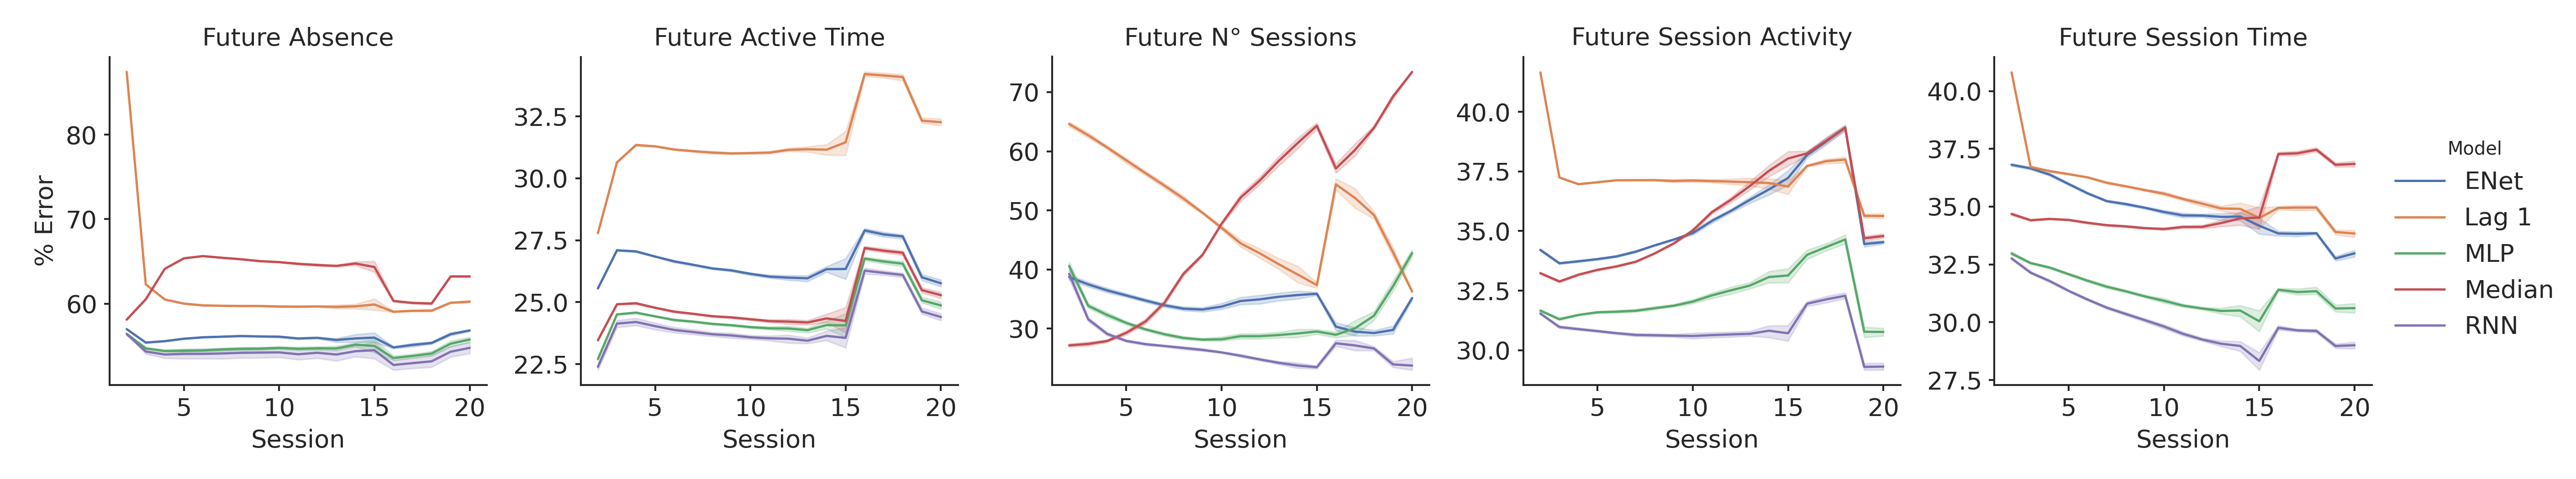
\includegraphics[width=0.9\textwidth]{images/chapter_3/models_comparison_collapsed_game_32.png}
\caption[\textbf{Model comparison collapsing over game context}]{ Overall, our approach (RNN) outperforms all the competing approaches at every time horizon. Each column represent the performance of the considered models on a specific target. Solid lines indicate the expected \% error over time for a specific combination of target and model. Dashed areas indicate the standard error of the mean.}
\label{model_comp_coll_game_32}
\end{figure}

Similar conclusions can be drawn from inspecting the performance over the game-context dimension, Figure \ref{model_comp_coll_time_32}, where the RNN achieved the lowest error rate in almost every game context-target combination. In the few occasions in which this was not the case the performance was at least comparable with that of the MLP architecture (although always better when looking at the expected performance).

\begin{figure}[h]
\centering
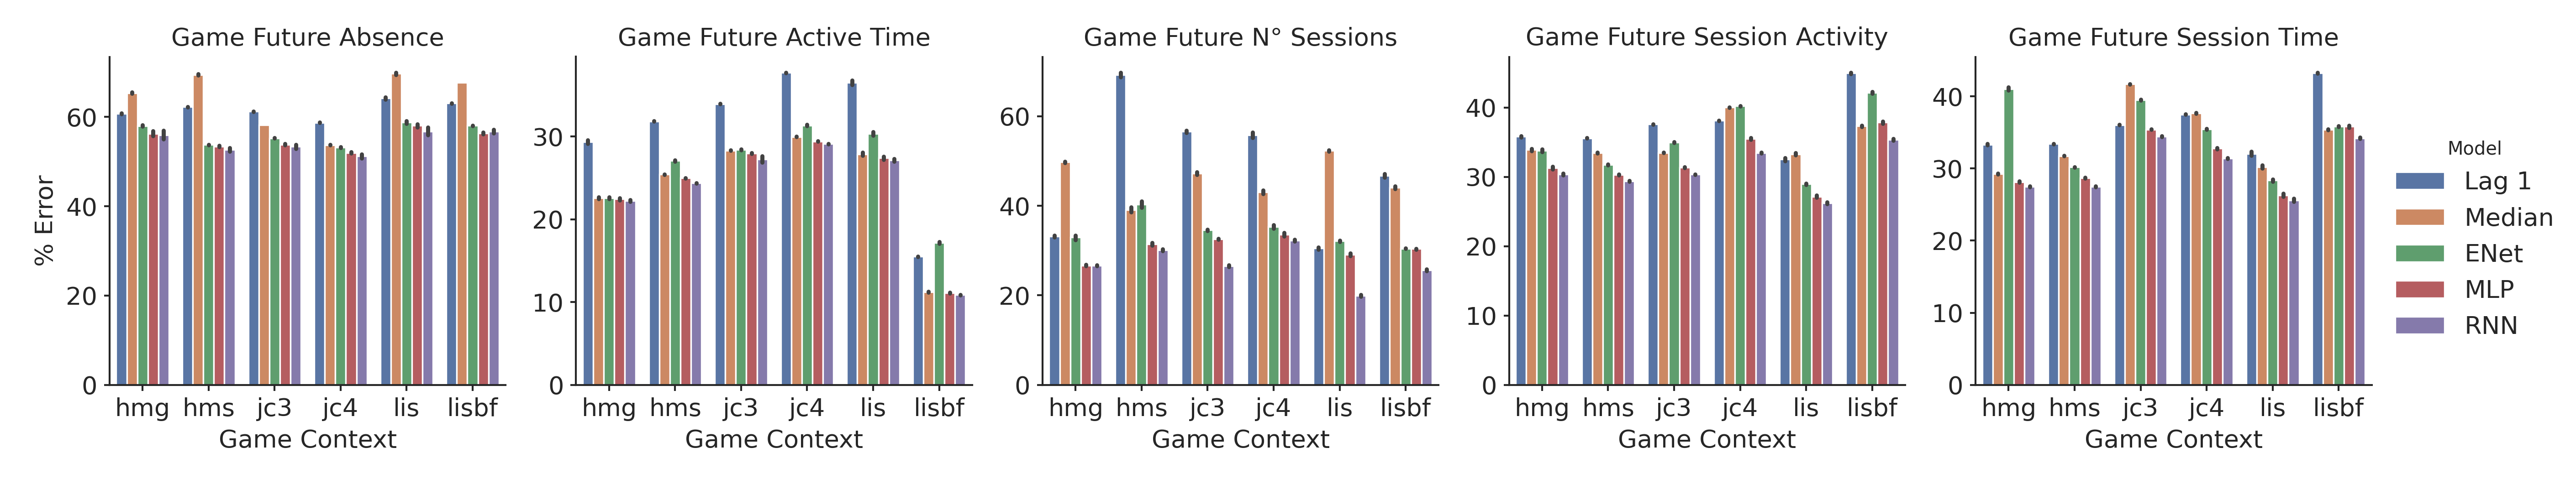
\includegraphics[width=0.9\textwidth]{images/chapter_3/models_comparison_collapsed_time_32.png}
\caption[\textbf{Model comparison collapsing over time}]{ Overall, our approach (RNN) outperforms all the competing approaches in most of the target-game context combinations. Each column represent the performance of the considered models on a specific target. Bars indicate the expected \% error for a specific combination of game context, target and model. Black vertical lines indicate the standard error of the mean.}
\label{model_comp_coll_time_32} 
\end{figure}

These results remain almost unchanged even wen considering the interaction between game context and time (see Figure \ref{model_comp_non_coll_32}).

\begin{figure}[h]
\centering
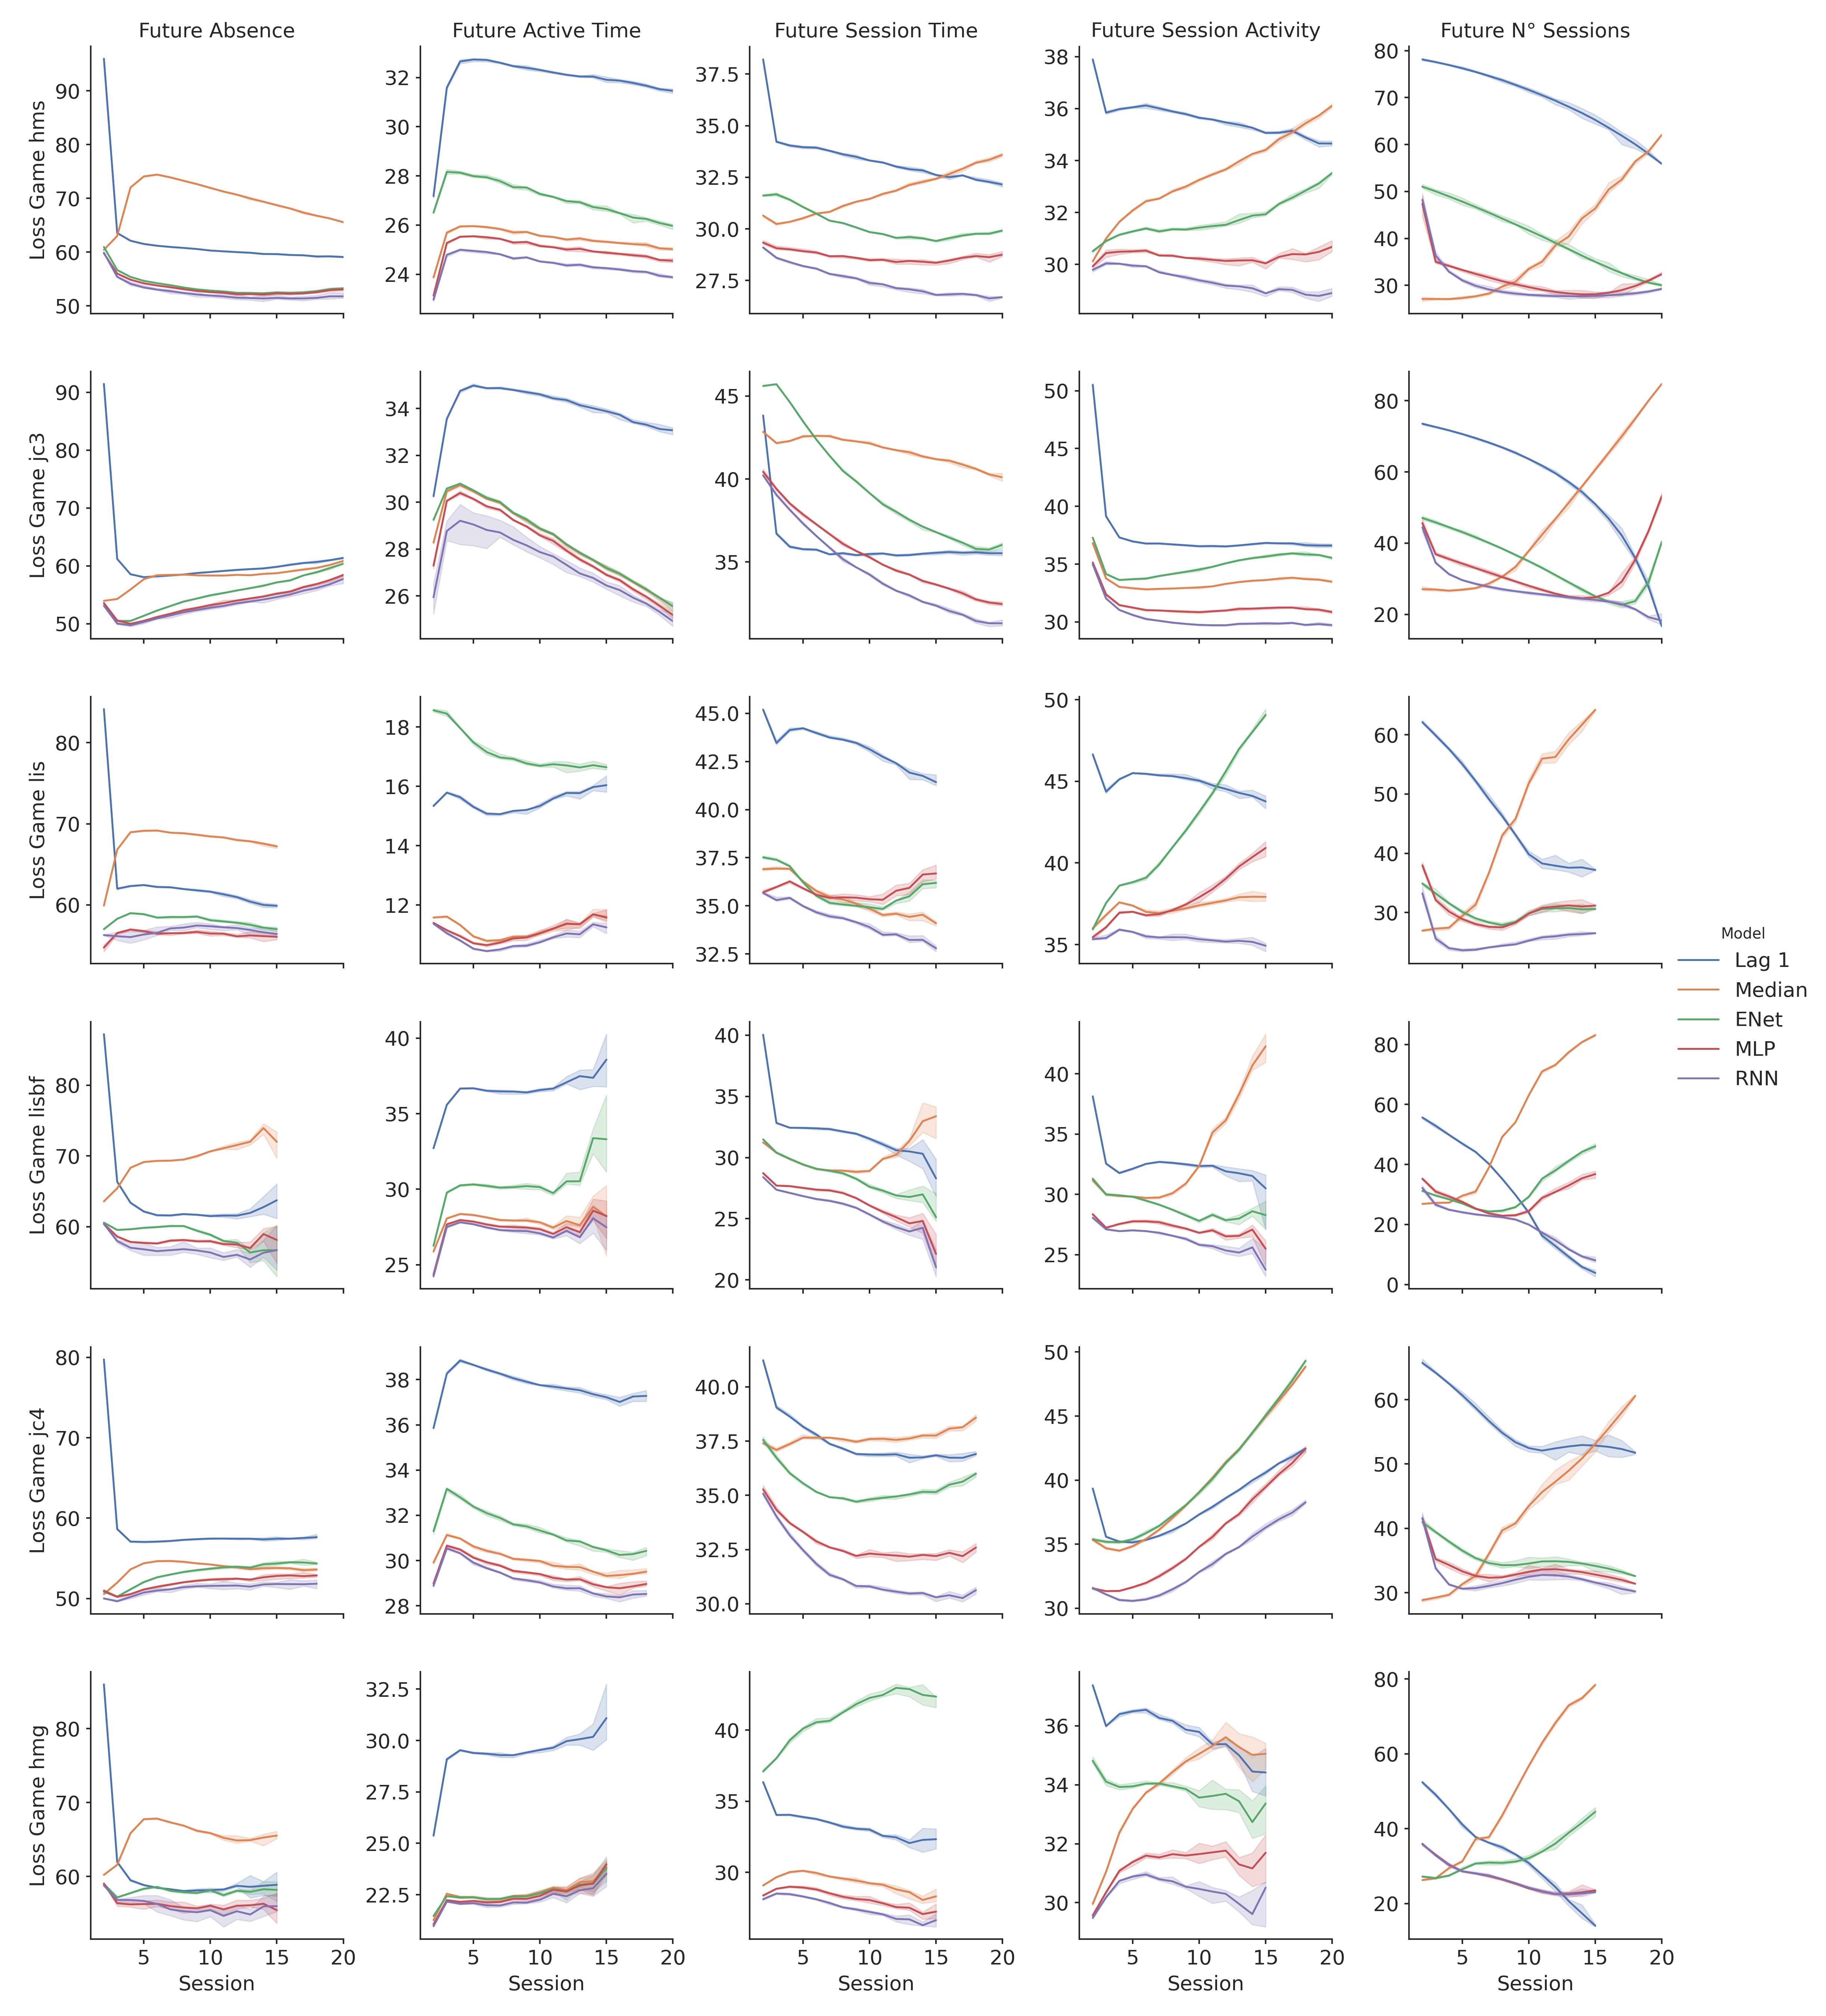
\includegraphics[height=0.7\textheight,keepaspectratio]{images/chapter_3/models_comparison_non_collapsed_32.png}
\caption[\textbf{Model comparison without collapsing}]{ Overall, our approach (RNN) outperforms all the competing approaches in most of the target-game context combinations and temporal horizons. Each column represents the performance of the considered models on a specific target while each row reports the performance on a specific game context. Solid lines indicate the expected \% error over time for a specific combination of target and model. Dashed areas indicate the standard error of the mean.}
\label{model_comp_non_coll_32} 
\end{figure}

At the level of global performance the RNN model markedly outperformed all competing approaches as clearly shown in Figure \ref{model_comp_coll_32}. This can be also seen in the results of the regression (see Table \ref{collapsed_lmm_32}) and  \textit{post hoc} analysis (see Table \ref{collapsed_post_hoc_32}). From the \textit{post hoc} analysis we can also observe how all the pairwise hypotheses presented in paragraph \ref{tuning_comparison_2} are confirmed. Here model performance is given by the sum of all the losses produced by the five targets and therefore provides a general indicator of model fit where lower values indicate a better performance overall.

\begin{figure}[h]
\centering
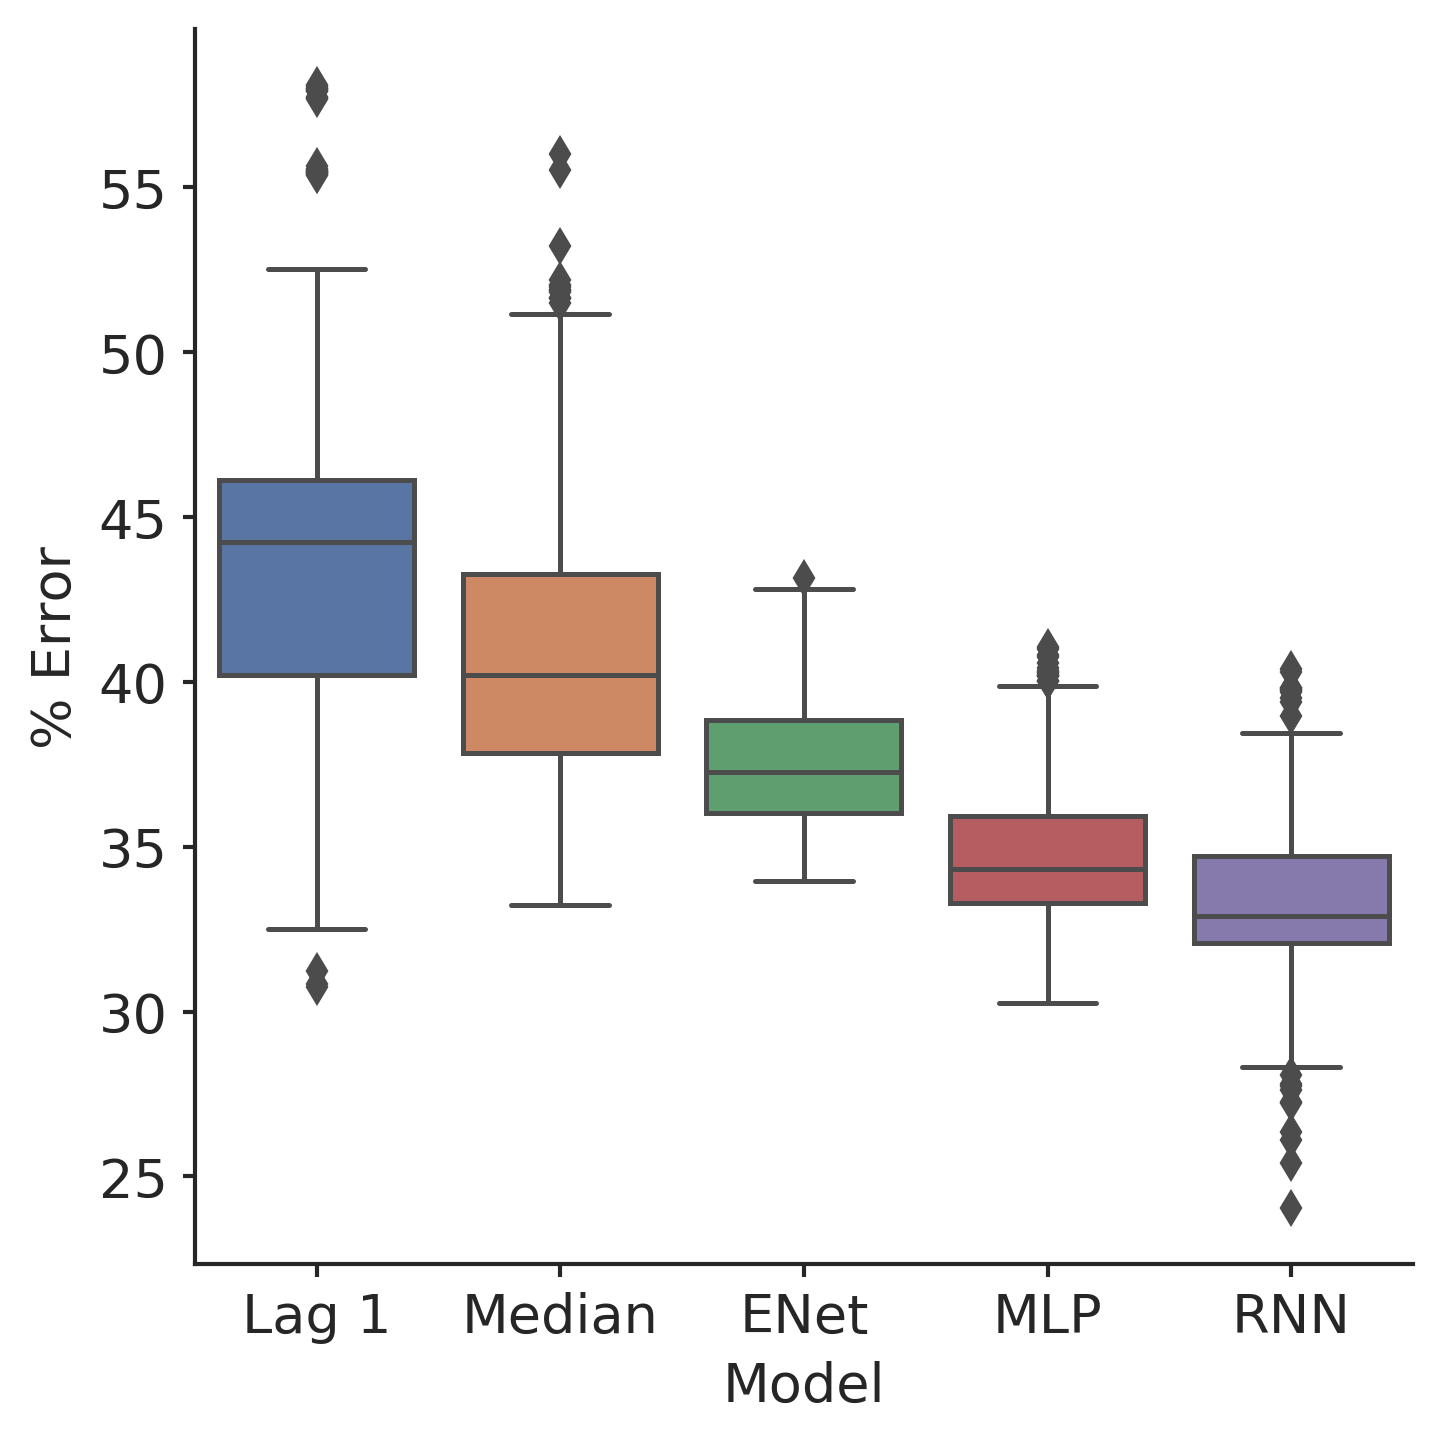
\includegraphics[width=.5\columnwidth]{images/chapter_3/performance_collapsed_32.png}
\caption[\textbf{Aggregated comparison of model performance}]{ Overall, our approach (RNN) outperforms all the competing approaches. Box-plots show the 10-fold cross-validation performance expressed as the total percentage of error (i.e. SMAPE) of each model over the five targets.}
\label{model_comp_coll_32} 
\end{figure}

\begin{table}[h]
\centering
\caption{Results of LMM on Collapsed Targets (Sum)}
\label{collapsed_target_lmm}
\resizebox{0.5\textwidth}{!}{
\begin{tabular}{ccccc}
\hline
\textbf{Model}           & \textbf{$\beta$} & \textbf{Z} & \textbf{p} & \textbf{95\% C.I.} \\ \hline
\multicolumn{5}{c}{\textbf{Collapsed Targets (Sum)}}                                                 \\ \hline
\textbf{Intercept (RNN)} & 33.129                & 41.799     & \textless .01   & 31.575 - 34.682      \\
\textbf{Lag 1}           & 10.010                 & 80.023     & \textless .01   & 9.765 - 10.255        \\
\textbf{Median}          & 7.482                 & 59.813     & \textless .01   & 7.237 - 7.727        \\
\textbf{ENet}            & 4.189                 & 33.491     & \textless .01   & 3.944 - 4.435        \\
\textbf{MLP}             & 1.411                 & 11.280     & \textless .01   & 1.166 - 1.656        \\ \hline
\end{tabular}
}
\end{table}

\begin{table}[h]
\centering
\caption{LMM Post-Hoc on Collapsed Targets (Sum)}
\label{collapsed_target_lmm_post_hoc}
\begin{tabular}{ccccc}
\hline
\textbf{Contrast}           & \textbf{$\beta_1$ - $\beta_2$} & \textbf{Z} & \textbf{p} & \textbf{95\% C.I.} \\ \hline
\multicolumn{5}{c}{\textbf{Collapsed Targets (Sum)}}                                                 \\ \hline
\textbf{Lag 1 - Median} & 2.528                & 20.210     & \textless .01   & 2.283 - 2.773      \\
\textbf{Median - ENet}          & 3.292                 & 26.322     & \textless .01   & 3.048 - 3.538        \\
\textbf{ENet - MLP}          & 2.778                 & 22.211     & \textless .01   & 2.533 - 3.024        \\ \hline
\end{tabular}
\end{table}

The superiority of the RNN model can still be observed when comparing the models on each target separately. However, the size of the effect varies depending on the target (see Table \ref{exploded_lmm_32}). The same trend is also present in the \textit{post hoc} analysis (see Table \ref{exploded_post_hoc_32}) where we observe only a partial confirmation of the pairwise hypotheses. The ENet model is outperformed by the Median baseline for three targets, namely Future Active Time, Session Time and Session Activity. All the coefficients in the regression analyses and the differences in the \textit{post hoc} analyses are non-standardized and can be interpreted as absolute changes in percentage error (i.e. SMAPE). 

In order to make these values more easily interpretable, we can use the information Table \ref{game_description_32}. For example, knowing that the median Session Time for the jc3 object is 162 minutes we can derive that when the RNN model achieves a SMAPE of 30\% in predicting Future Session Time, this equates on average to an absolute error of $1.62 \times 30 \sim 48$ minutes. All the p-values in the \textit{post hoc} analyses are Bonferroni corrected for multiple comparisons. 

The results of the statistical analyses suggest positive additive effects of non-linearity and recurrency on model performance both at the level of global and target-specific performance. This effect is more pronounced for certain targets (e.g. Future Session Time, Future N° Sessions) than for others (e.g. Future Absence, Future Active Time). Moreover, looking at Figure \ref{model_comp_exp_32} it appears that RNN improved on MLP (i.e., the second best model) using roughly half the parameters and per-epoch computation time. 

\begin{table}[h]
\centering
\caption{Results of LMM on Non-Collapsed Targets}
\label{exploded_target_lmm}
\begin{tabular}{ccccc}
\hline
\textbf{Model}  & \textbf{$\beta$} & \textbf{Z} & \textbf{p} & \textbf{95\% C.I.}                  \\ \hline
\multicolumn{5}{c}{\textbf{Future Absence}}                                                                         \\ \hline
\textbf{Intercept (RNN)} & 54.46                & 144.316     & \textless .01   & 53.72 - 55.20                     \\
\textbf{Lag 1}           & 7.40                & 40.509     & \textless .01   & 7.04 - 7.76                     \\
\textbf{Median}          & 9.47                & 51.814     & \textless .01   & 9.11 - 9.83                     \\
\textbf{ENet}            & 1.71                & 9.353     & \textless .01   & 1.35 - 2.06                     \\
\textbf{MLP}             & .53                & 2.915     & \textless .01   & .175 - .891                       \\ \hline
\multicolumn{5}{c}{\textbf{Future Active Time}}                                                                     \\ \hline
\textbf{Intercept (RNN)} & 23.36                & 20.019      & \textless .01  & 21.78 - 24.93                     \\
\textbf{Lag 1}           & 7.32               & 119.028    & \textless .01  & 7.2 - 7.44                     \\
\textbf{Median}          & .77                & 12.515     & \textless .01  & .649 - .891                     \\
\textbf{ENet}            & 2.55                & 41.551     & \textless .01  & 2.43 - 2.67                     \\
\textbf{MLP}             & .41                & 6.739      & \textless .01  & .294 - .535                     \\ \hline
\multicolumn{5}{c}{\textbf{Future Session Time}}                                                                     \\ \hline
\textbf{Intercept (RNN)} & 30.02                & 63.663     & \textless .01  & 29.1 - 30.95                     \\
\textbf{Lag 1}            & 5.62                & 49.158     & \textless .01  & 5.39 - 5.83                     \\
\textbf{Median}          & 4.45                & 38.957     & \textless .01  & 4.23 - 4.67                     \\
\textbf{ENet}            & 4.81                & 42.098     & \textless .01  & 4.59 - 5.03                     \\
\textbf{MLP}             & 1.08                & 9.529      & \textless .01  & .86 - 1.31                     \\ \hline
\multicolumn{5}{c}{\textbf{Future Session Activity}}                                                                 \\ \hline
\textbf{Intercept (RNN)} & 31.04                & 70.241     & \textless .01  & \multicolumn{1}{l}{30.17 - 31.9} \\
\textbf{Lag 1}            & 6.52                & 61.025     & \textless .01  & \multicolumn{1}{l}{6.31 - 6.73} \\
\textbf{Median}          & 4.37                & 40.879     & \textless .01  & \multicolumn{1}{l}{4.16 - 4.58} \\
\textbf{ENet}            & 4.42                & 41.319     & \textless .01  & \multicolumn{1}{l}{4.21 - 4.63} \\
\textbf{MLP}             & 1.36                & 12.762     & \textless .01  & \multicolumn{1}{l}{1.15 - 1.57} \\ \hline
\multicolumn{5}{c}{\textbf{Future N° Sessions}}                                                                      \\ \hline
\textbf{Intercept (RNN)} & 26.77                & 7.445     & \textless .01  & 19.72 - 33.81                     \\
\textbf{Lag 1}            & 23.17                & 44.430     & \textless .01  & 22.15 - 24.19                     \\
\textbf{Median}          &  18.34              & 35.166     & \textless .01  & 17.31 - 19.36                     \\
\textbf{ENet}            & 7.44                & 14.277     & \textless .01  & 6.42 - 8.46                     \\
\textbf{MLP}             & 3.65                & 7.005      & \textless .01  & 2.63 - 4.67                       \\ \hline
\end{tabular}
\end{table}

\begin{table}[h]
\centering
\caption{LMM Post-Hoc on Non-Collapsed Targets}
\label{exploded_target_lmm_post_hoc}
\begin{tabular}{ccccc}
\hline
\textbf{Contrast}  & \textbf{$\beta_1$-$\beta_2$} & \textbf{Z} & \textbf{p} & \textbf{95\% C.I.}                  \\ \hline
\multicolumn{5}{c}{\textbf{Future Absence}}                                                                         \\ \hline
\textbf{Lag 1 - Median} & -2.06                & -11.305     & \textless .01   & -2.42 - -1.70                     \\
\textbf{Median - ENet}           & 7.76                & 42.461     & \textless .01   & 7.40 - 8.12                     \\
\textbf{ENet - MLP}          & 1.17                & 6.438     & \textless .01   & .81 - 1.535                    \\ \hline
\multicolumn{5}{c}{\textbf{Future Active Time}}                                                                     \\ \hline
\textbf{Lag 1 - Median} & 6.55                & 106.513      & \textless .01  & 6.433 - 6.67                     \\
\textbf{Median - ENet}           & -1.78                & -29.037    & \textless .01  & -1.9 - -1.66                     \\
\textbf{ENet - MLP}          & 2.14                & 34.812     & \textless .01  & 2.02 - 2.26                     \\\hline
\multicolumn{5}{c}{\textbf{Future Session Time}}                                                                     \\ \hline
\textbf{Lag 1 - Median} & 1.16                & 10.201     & \textless .01  & .94 - 1.39                     \\
\textbf{Median - ENet}            & -.35                & -3.141     & \textless .01  & -.58 - -.13                     \\
\textbf{ENet - MLP}          & 3.72                & 32.579     & \textless .01  & 3.5 - 3.95                     \\ \hline
\multicolumn{5}{c}{\textbf{Future Session Activity}}                                                                 \\ \hline
\textbf{Lag 1 - Median} & 2.15                & 20.146     & \textless .01  & \multicolumn{1}{l}{1.94 - 2.36} \\
\textbf{Median - ENet}            & -.04                & -.441     &  1.  & \multicolumn{1}{l}{-.257 - .163} \\
\textbf{ENet - MLP}          & 3.05                & 28.558     & \textless .01  & \multicolumn{1}{l}{2.84 - 3.26} \\ \hline
\multicolumn{5}{c}{\textbf{Future N° Sessions}}                                                                      \\ \hline
\textbf{Lag 1 - Median} & 4.83                & 9.264     & \textless .01  & 3.8 - 5.85                     \\
\textbf{Median - ENet}            & 10.89                & 20.889     & \textless .01  & 9.87 - 11.91                     \\
\textbf{ENet - MLP}          & 3.79                & 7.272     & \textless .01  & 2.77 - 4.81                     \\\hline
\end{tabular}
\end{table}

\begin{figure*}[h]
\centering
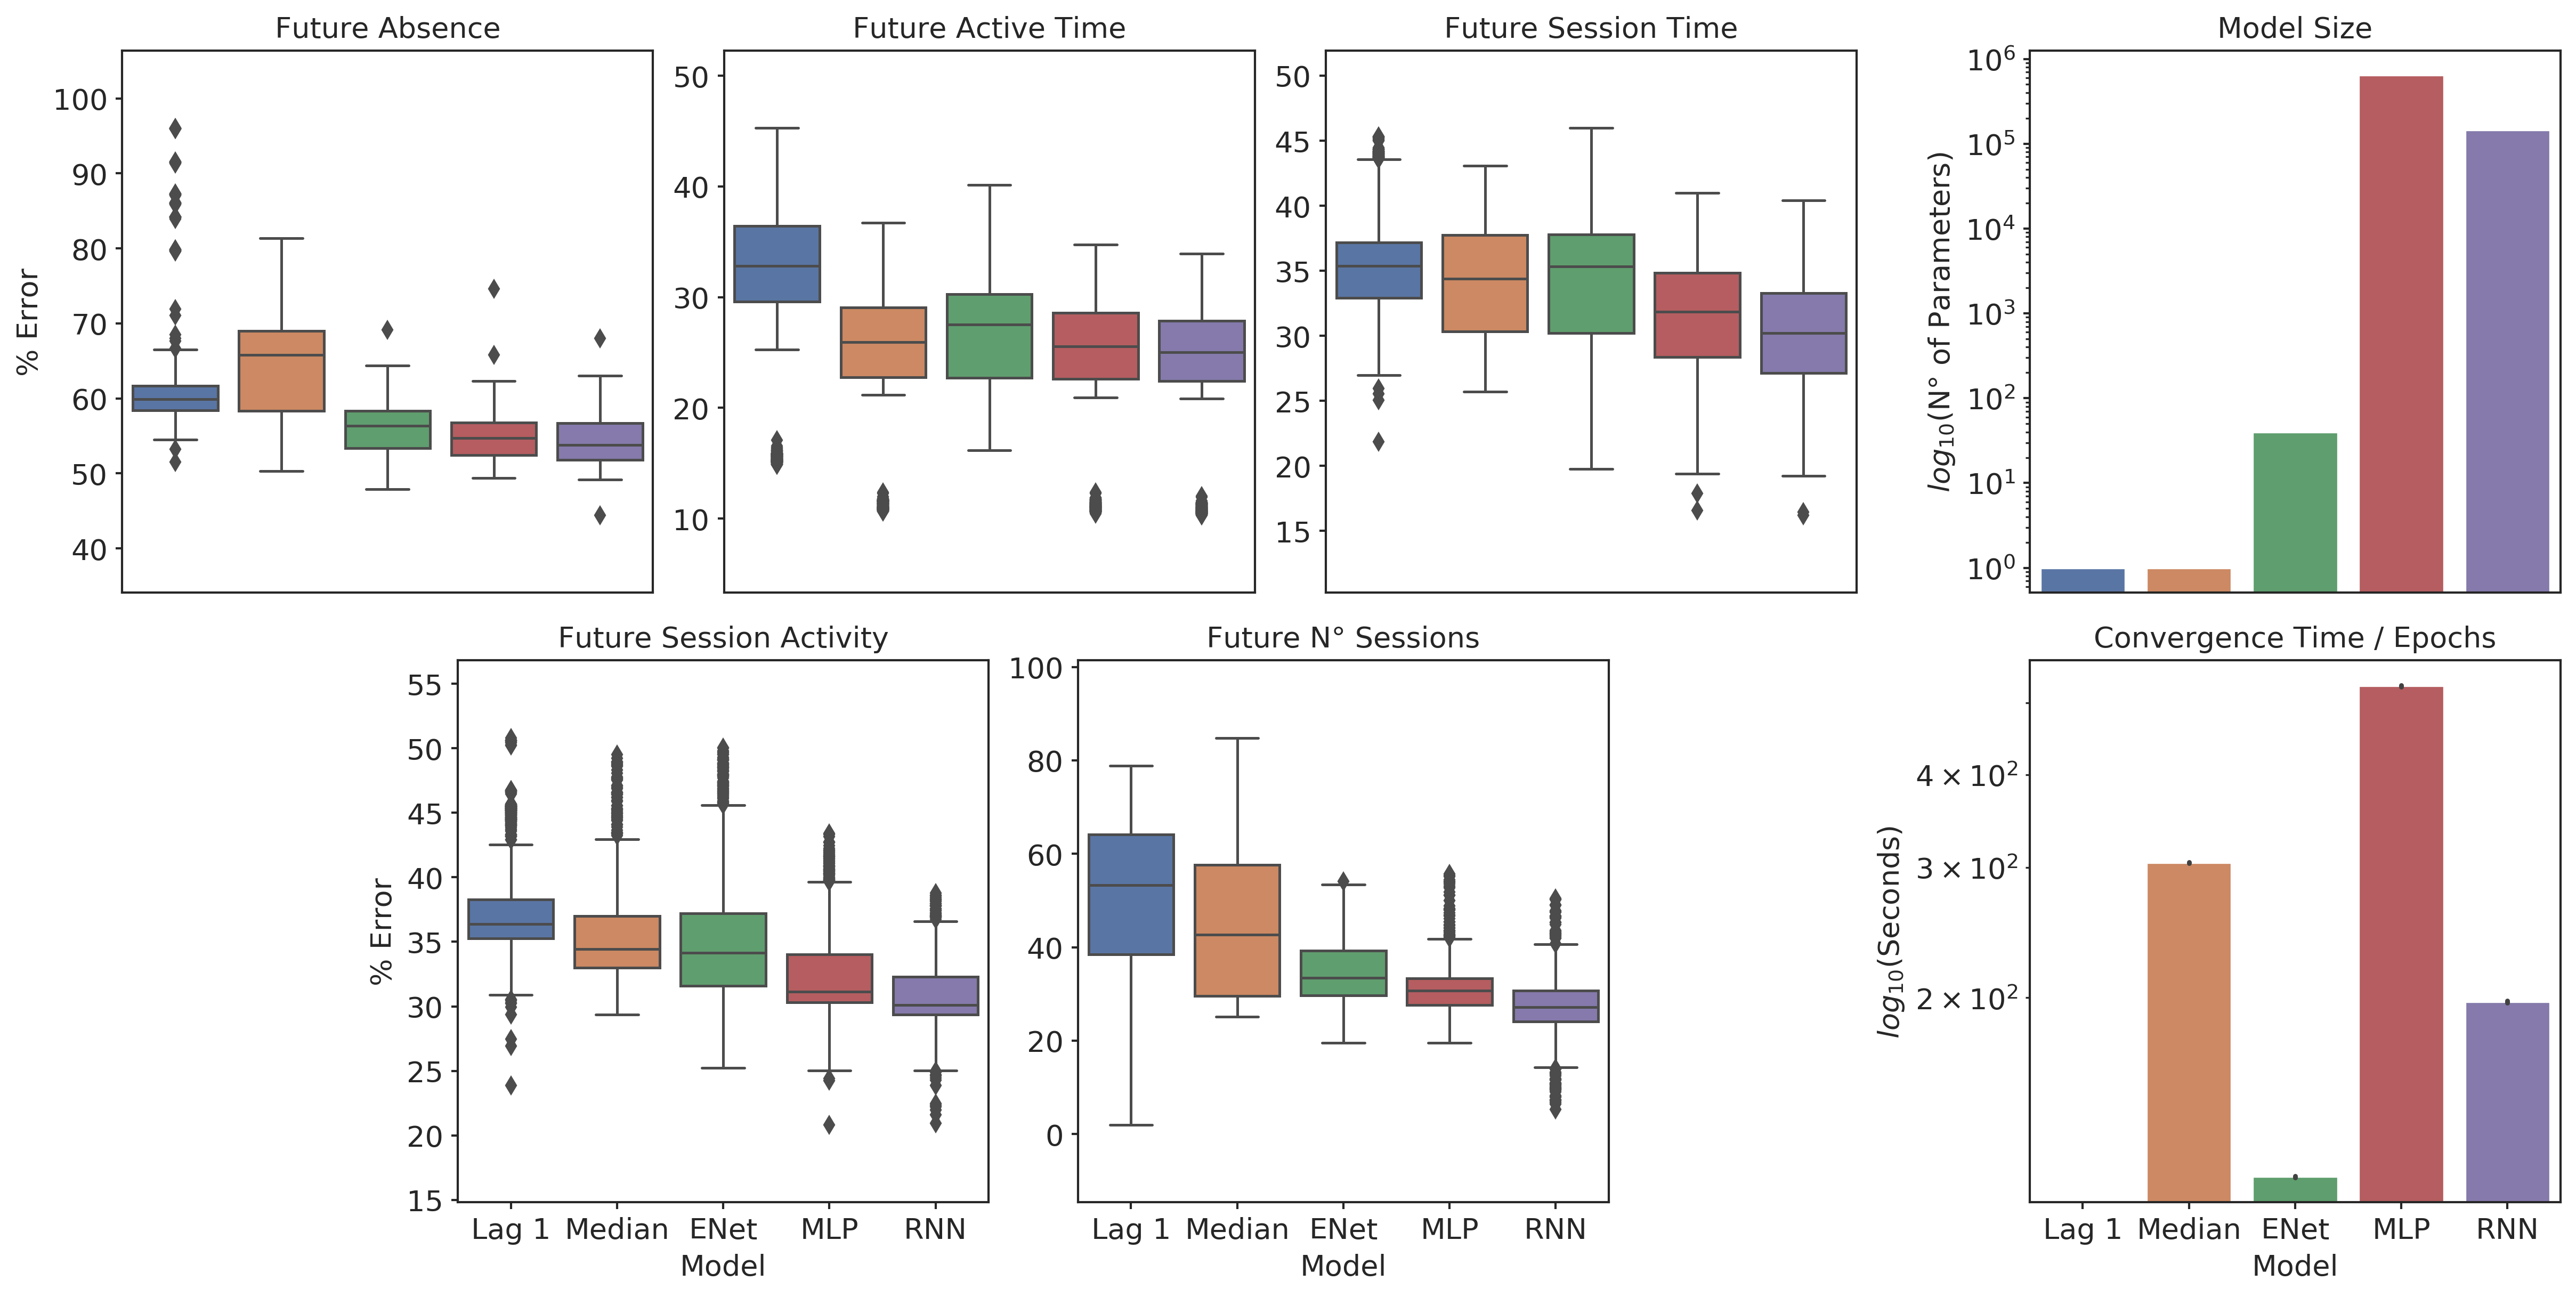
\includegraphics[width=.7\textwidth]{images/chapter_3/performance_exploded_32.png}
\caption[\textbf{Dis-aggregated comparison of models' performance}]{Our approach (RNN) outperformed all competing ones on each target. It consistently used fewer parameters and had shorter computation time than the second best performing model. Box-plots show the 10-fold cross-validation performance expressed as percentage of error (i.e. SMAPE) of each model for the five targets. The bar-plot on the top row indicates the number of free parameters for each model while the bar plot on the bottom row shows the average time for each training epoch. Both bar-plots are $log_{10}$ scaled.}
\label{model_comp_exp_32} 
\end{figure*}

\subsection{Model Criticism}
\label{model_criticims_2}
Similarly to what presented in section \ref{results_1} we were able to observe different level of performance for the baseline models in different game contexts, suggesting once again heterogeneity in the level of challenge for the predictive task. A similar level of heterogeneity was also found among the considered behavioural targets (e.g. Future Absence appeared to be a much harder target to predict than Future N° of Sessions) and temporal horizons (e.g. predictions made at an early or late stage showed to be more or less challenging depending on the considered target, game context and model architecture). By looking at the performance of the various parametric models we were able to replicate our initial findings, suggesting the importance of modelling non-linear dynamics when predicting measures of future behavioural intensity. When a model provided better performance than a competing one it did so among all the considered game contexts and behavioural targets, again confirming that the adopted global multi-task learning approach did not cause any degradation in predictive accuracy. 

In summary, improving the BM model and modifying its architecture in order to better incorporate the theoretical constrains outlined in chapter \ref{chapter_theory_modelling} did not substantially change any of the findings reported in the first iteration of the model building process. 

That said, despite the RNN architecture was now able to generate representations compatible with the computational frameworks presented by McClure et al. \cite{mcclure2003computational} and Zhang et al. \cite{zhang2009neural} it was still not taking into account factors that might be relevant for reliably estimating the level of attributed incentive salience. Indeed, as we mentioned in chapter \ref{chapter_lit_review}, we know that this type of latent state, and its associated dynamics, are modulated by the internal condition of the individual \cite{zhang2009neural}, by the characteristics of the rewarding object (a specific videogame in this case) with which the individual is interacting and by the environment in which the interaction is occurring \cite{palminteri2015contextual}. These factors, were only partially and indirectly captured by the RNN architecture as they require more granular information (i.e., in-game and environmental information) and with a higher temporal resolution (i.e., within rather than between game sessions). As a consequence we noticed how the RNN architecture, despite outperforming competing ones, still achieved a relatively high error rate in predicting some of the considered behavioural targets (e.g., future Absence). 

A possible solution in this case would have been to incorporate information about the environment in which the observed behaviour occurred (e.g., time and location of a specific game session) and about the characteristics of the rewarding objects (i.e., the so called videogame structural characteristics that we mentioned in chapter \ref{chapter_lit_review}). As well as improving the predictive performance of the model, these new types of information should also increase the quality of the generated representation and consequently allow for a better approximation of the level of attributed incentive salience. In line with the ideas presented in section \ref{modelling_env_and_game_elements}, the next iteration of the model building process will aim at modifying the RNN architecture in order to incorporate the type of environmental and game-specific information that we just mentioned.

\section{Dynamic Prediction of Future Behavioural Intensity with Environmental and Game Covariates}
\label{model_architecture_3}
In the third and last iteration of the model building process the focus was mostly on modifying the RNN architecture in order to incorporate information from the environment surrounding the individual and the in-game events characterizing the playing sessions. However, given the computational flexibility of ANN, this needed to be done through a strategy that maintained compliance with the theoretical constrains mentioned in chapter \ref{chapter_theory_modelling}.

Our approach was then to assume that the amount of incentive salience that an individual attributes to a potentially rewarding object (i.e., a videogame) during a specific interaction could be decomposed in 3 major components:
\begin{enumerate}
    \item The current level of attributed incentive salience. This can be inferred by the history of interactions an their associated behavioural intensity. In our setting this was represented by the latent state inferred by the model after observing all the previous interactions.
    \item The impact of the environmental conditions in which each interaction occurred. This information does not directly influence the amount of attributed incentive salience but help accounting for discrepancies in the observed behavioural manifestations. For example, an individual might ascribe high saliency to a specific object but show reduced goal directed behaviour due to impediments in the surrounding environment. In our setting these were represented by a series of indicators (e.g., hour of day, day of the week ) specifying the environmental conditions in which a playing session was observed.
    \item The impact of the, potentially rewarding, characteristics of the object. This factor is directly involved in determining the level of attributed saliency as it informs about which aspects of the game are likely to produce rewarding experiences. In our setting these were represented by metrics describing the amount and type of game events triggered by an individual during a playing session. It is important to note that given the nature of video games (i.e., secondary rewarding objects) the impact of these characteristics could vary from individual to individual and from interaction to interaction. In this view they are better understood in conjunction with the behavioural intensity of the game session in which they occur. For example, if an individual produces a prolonged playing session characterized by a high number of exploration events, it is likely that in this instance these specific characteristics contributed to the rewarding experience provided by the game.
\end{enumerate}

By adopting a similar approach to Neural GAMs \cite{agarwal2021neural} each component was estimated independently and subsequently combined in a single, more informative, representation. This was done with the aim to achieve a higher level of predictive accuracy while maintaining control on the mechanics generating the latent representation (more details will be provided in section \ref{model_design_3}). 

In order to investigate the contribution of the included covariates in improving the overall predictive accuracy we proceeded at validating the following hypotheses:
\begin{enumerate}
    \item Including information about the environmental context in which an interaction occurred can have a positive impact on the predictive accuracy of the model.
    \item Including information about the amount and type of game events occurring during an interaction can increase predictive accuracy more than when considering environmental factors alone. 
    \item Considering the joint contribution of environmental factors and game characteristics can have a greater impact on predictive accuracy than when considering the two factors alone.  
\end{enumerate}

We want to stress how in this context we considered the ability to account for temporal dynamics as a factor of pivotal importance. The model had now to track changes not just in the behavioural intensity of the observed interactions, but also in the surrounding environment and in the preference for different game characteristics. For this reason we also tried to replicate some of the findings observed in the previous stages of the model building process by evaluating the following additional hypotheses

\begin{enumerate}
    \item Including sequential dynamics in the modelling approach can have a positive effect on the predictive performance.
    \item It is possible to have a single model jointly multiple first-order metrics of behavioural intensity without any substantial loss in accuracy
    \item It is possible to have a single model performing the predictive task simultaneously across a wide range of games.
\end{enumerate}

\subsection{Model Design}
\label{model_design_3}
The final iteration of our ANN architecture was an extension of the previous RNN model and aimed to jointly predict the same set of 5 behavioural metrics. This new architecture however, leveraging the same principles of Neural GAMs (as outlined in section \ref{modelling_env_and_game_elements}), tried to obtain a better estimate of the latent state used for predicting future behaviour by decomposing it in 3 functional components. The architecture is illustrated in Figure \ref{fig: rnn_env_even}

\begin{figure}[ht]
\begin{center}
\begin{adjustbox}{width=0.7\textwidth}
    \tikzset{every picture/.style={line width=0.75pt}} %set default line width to 0.75pt        
    
    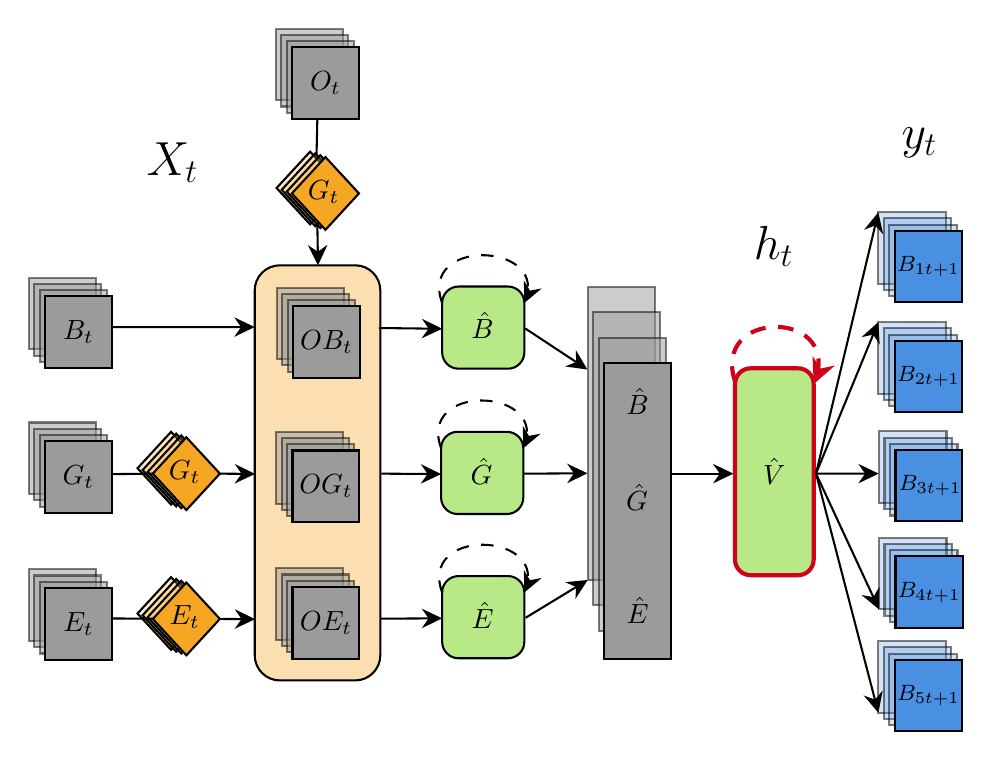
\begin{tikzpicture}[x=0.75pt,y=0.75pt,yscale=-1,xscale=1]
    %uncomment if require: \path (0,411); %set diagram left start at 0, and has height of 411
    
    %Rounded Rect [id:dp15650356150345013] 
    \draw  [fill={rgb, 255:red, 245; green, 166; blue, 35 }  ,fill opacity=0.36 ] (219.9,142.15) .. controls (219.9,135.47) and (225.32,130.05) .. (232,130.05) -- (268.3,130.05) .. controls (274.98,130.05) and (280.4,135.47) .. (280.4,142.15) -- (280.4,317.95) .. controls (280.4,324.63) and (274.98,330.05) .. (268.3,330.05) -- (232,330.05) .. controls (225.32,330.05) and (219.9,324.63) .. (219.9,317.95) -- cycle ;
    %Straight Lines [id:da409284418173784] 
    \draw    (250.06,109.76) -- (250.35,127.05) ;
    \draw [shift={(250.4,130.05)}, rotate = 269.03] [fill={rgb, 255:red, 0; green, 0; blue, 0 }  ][line width=0.08]  [draw opacity=0] (9.82,-4.72) -- (0,0) -- (9.82,4.72) -- (6.52,0) -- cycle    ;
    %Shape: Rectangle [id:dp7034345660290355] 
    \draw  [color={rgb, 255:red, 0; green, 0; blue, 0 }  ,draw opacity=0.5 ][fill={rgb, 255:red, 155; green, 155; blue, 155 }  ,fill opacity=0.5 ] (111.01,276.53) -- (143.26,276.53) -- (143.26,311.05) -- (111.01,311.05) -- cycle ;
    %Shape: Rectangle [id:dp22118233628007533] 
    \draw  [color={rgb, 255:red, 0; green, 0; blue, 0 }  ,draw opacity=0.5 ][fill={rgb, 255:red, 155; green, 155; blue, 155 }  ,fill opacity=0.5 ] (113.63,279.51) -- (145.88,279.51) -- (145.88,314.03) -- (113.63,314.03) -- cycle ;
    %Shape: Rectangle [id:dp24867768000931467] 
    \draw  [color={rgb, 255:red, 0; green, 0; blue, 0 }  ,draw opacity=0.5 ][fill={rgb, 255:red, 155; green, 155; blue, 155 }  ,fill opacity=0.5 ] (116.27,282.56) -- (148.53,282.56) -- (148.53,317.08) -- (116.27,317.08) -- cycle ;
    %Shape: Rectangle [id:dp124905579804508] 
    \draw  [fill={rgb, 255:red, 155; green, 155; blue, 155 }  ,fill opacity=1 ] (118.86,285.5) -- (151.11,285.5) -- (151.11,320.02) -- (118.86,320.02) -- cycle ;
    %Straight Lines [id:da8537240673366849] 
    \draw    (250.06,59.86) -- (249.67,77.43) ;
    %Rounded Rect [id:dp9724403504665806] 
    \draw  [color={rgb, 255:red, 208; green, 2; blue, 27 }  ,draw opacity=1 ][fill={rgb, 255:red, 184; green, 233; blue, 134 }  ,fill opacity=1 ][line width=1.5]  (451.3,187.25) .. controls (451.3,183.06) and (454.7,179.67) .. (458.88,179.67) -- (481.62,179.67) .. controls (485.81,179.67) and (489.2,183.06) .. (489.2,187.25) -- (489.2,271.79) .. controls (489.2,275.97) and (485.81,279.37) .. (481.62,279.37) -- (458.88,279.37) .. controls (454.7,279.37) and (451.3,275.97) .. (451.3,271.79) -- cycle ;
    %Curve Lines [id:da6973720397061056] 
    \draw [color={rgb, 255:red, 208; green, 2; blue, 27 }  ,draw opacity=1 ][line width=1.5]  [dash pattern={on 5.63pt off 4.5pt}]  (451.3,186.02) .. controls (439.95,151.4) and (500.2,151.33) .. (490.53,183.61) ;
    \draw [shift={(489.2,187.25)}, rotate = 293.32] [fill={rgb, 255:red, 208; green, 2; blue, 27 }  ,fill opacity=1 ][line width=0.08]  [draw opacity=0] (12.23,-5.88) -- (0,0) -- (12.23,5.88) -- (8.12,0) -- cycle    ;
    %Shape: Rectangle [id:dp1958055080757597] 
    \draw  [color={rgb, 255:red, 0; green, 0; blue, 0 }  ,draw opacity=0.5 ][fill={rgb, 255:red, 74; green, 144; blue, 226 }  ,fill opacity=0.25 ] (520.36,157.39) -- (552.87,157.39) -- (552.87,191.9) -- (520.36,191.9) -- cycle ;
    %Shape: Rectangle [id:dp20825701586292622] 
    \draw  [color={rgb, 255:red, 0; green, 0; blue, 0 }  ,draw opacity=0.5 ][fill={rgb, 255:red, 74; green, 144; blue, 226 }  ,fill opacity=0.25 ] (523,160.37) -- (555.51,160.37) -- (555.51,194.88) -- (523,194.88) -- cycle ;
    %Shape: Rectangle [id:dp6709034910590727] 
    \draw  [color={rgb, 255:red, 0; green, 0; blue, 0 }  ,draw opacity=0.5 ][fill={rgb, 255:red, 74; green, 144; blue, 226 }  ,fill opacity=0.25 ] (525.67,163.42) -- (558.17,163.42) -- (558.17,197.93) -- (525.67,197.93) -- cycle ;
    %Shape: Rectangle [id:dp943426610209301] 
    \draw  [fill={rgb, 255:red, 74; green, 144; blue, 226 }  ,fill opacity=1 ] (528.28,166.36) -- (560.78,166.36) -- (560.78,200.87) -- (528.28,200.87) -- cycle ;
    %Shape: Rectangle [id:dp9270730461824767] 
    \draw  [color={rgb, 255:red, 0; green, 0; blue, 0 }  ,draw opacity=0.5 ][fill={rgb, 255:red, 74; green, 144; blue, 226 }  ,fill opacity=0.25 ] (520.69,210.06) -- (553.2,210.06) -- (553.2,244.56) -- (520.69,244.56) -- cycle ;
    %Shape: Rectangle [id:dp9671567967621458] 
    \draw  [color={rgb, 255:red, 0; green, 0; blue, 0 }  ,draw opacity=0.5 ][fill={rgb, 255:red, 74; green, 144; blue, 226 }  ,fill opacity=0.25 ] (523.33,213.04) -- (555.84,213.04) -- (555.84,247.54) -- (523.33,247.54) -- cycle ;
    %Shape: Rectangle [id:dp6567850092606636] 
    \draw  [color={rgb, 255:red, 0; green, 0; blue, 0 }  ,draw opacity=0.5 ][fill={rgb, 255:red, 74; green, 144; blue, 226 }  ,fill opacity=0.25 ] (526,216.09) -- (558.5,216.09) -- (558.5,250.6) -- (526,250.6) -- cycle ;
    %Shape: Rectangle [id:dp9307909660529495] 
    \draw  [fill={rgb, 255:red, 74; green, 144; blue, 226 }  ,fill opacity=1 ] (528.62,219.02) -- (560.84,219.02) -- (560.84,253.22) -- (528.62,253.22) -- cycle ;
    %Shape: Rectangle [id:dp2956426995252315] 
    \draw  [color={rgb, 255:red, 0; green, 0; blue, 0 }  ,draw opacity=0.5 ][fill={rgb, 255:red, 74; green, 144; blue, 226 }  ,fill opacity=0.25 ] (520.36,311.11) -- (552.87,311.11) -- (552.87,345.62) -- (520.36,345.62) -- cycle ;
    %Shape: Rectangle [id:dp9676718309145981] 
    \draw  [color={rgb, 255:red, 0; green, 0; blue, 0 }  ,draw opacity=0.5 ][fill={rgb, 255:red, 74; green, 144; blue, 226 }  ,fill opacity=0.25 ] (523,314.09) -- (555.51,314.09) -- (555.51,348.6) -- (523,348.6) -- cycle ;
    %Shape: Rectangle [id:dp3802447939611997] 
    \draw  [color={rgb, 255:red, 0; green, 0; blue, 0 }  ,draw opacity=0.5 ][fill={rgb, 255:red, 74; green, 144; blue, 226 }  ,fill opacity=0.25 ] (525.67,317.14) -- (558.17,317.14) -- (558.17,351.65) -- (525.67,351.65) -- cycle ;
    %Shape: Rectangle [id:dp2655409211543931] 
    \draw  [fill={rgb, 255:red, 74; green, 144; blue, 226 }  ,fill opacity=1 ] (528.28,320.08) -- (560.78,320.08) -- (560.78,354.59) -- (528.28,354.59) -- cycle ;
    %Shape: Rectangle [id:dp4040153422296009] 
    \draw  [color={rgb, 255:red, 0; green, 0; blue, 0 }  ,draw opacity=0.5 ][fill={rgb, 255:red, 74; green, 144; blue, 226 }  ,fill opacity=0.25 ] (520.69,261.32) -- (553.2,261.32) -- (553.2,295.83) -- (520.69,295.83) -- cycle ;
    %Shape: Rectangle [id:dp7066102537923638] 
    \draw  [color={rgb, 255:red, 0; green, 0; blue, 0 }  ,draw opacity=0.5 ][fill={rgb, 255:red, 74; green, 144; blue, 226 }  ,fill opacity=0.25 ] (523.33,264.3) -- (555.84,264.3) -- (555.84,298.81) -- (523.33,298.81) -- cycle ;
    %Shape: Rectangle [id:dp46050637304135866] 
    \draw  [color={rgb, 255:red, 0; green, 0; blue, 0 }  ,draw opacity=0.5 ][fill={rgb, 255:red, 74; green, 144; blue, 226 }  ,fill opacity=0.25 ] (526,267.35) -- (558.5,267.35) -- (558.5,301.86) -- (526,301.86) -- cycle ;
    %Shape: Rectangle [id:dp2033829273595421] 
    \draw  [fill={rgb, 255:red, 74; green, 144; blue, 226 }  ,fill opacity=1 ] (528.61,270.29) -- (561.11,270.29) -- (561.11,304.8) -- (528.61,304.8) -- cycle ;
    %Shape: Rectangle [id:dp19424752965877823] 
    \draw  [color={rgb, 255:red, 0; green, 0; blue, 0 }  ,draw opacity=0.5 ][fill={rgb, 255:red, 74; green, 144; blue, 226 }  ,fill opacity=0.25 ] (520.36,104.48) -- (552.87,104.48) -- (552.87,138.98) -- (520.36,138.98) -- cycle ;
    %Shape: Rectangle [id:dp6987771152166413] 
    \draw  [color={rgb, 255:red, 0; green, 0; blue, 0 }  ,draw opacity=0.5 ][fill={rgb, 255:red, 74; green, 144; blue, 226 }  ,fill opacity=0.25 ] (523,107.46) -- (555.51,107.46) -- (555.51,141.96) -- (523,141.96) -- cycle ;
    %Shape: Rectangle [id:dp12765942569283661] 
    \draw  [color={rgb, 255:red, 0; green, 0; blue, 0 }  ,draw opacity=0.5 ][fill={rgb, 255:red, 74; green, 144; blue, 226 }  ,fill opacity=0.25 ] (525.67,110.51) -- (558.17,110.51) -- (558.17,145.01) -- (525.67,145.01) -- cycle ;
    %Shape: Rectangle [id:dp16248810139444148] 
    \draw  [fill={rgb, 255:red, 74; green, 144; blue, 226 }  ,fill opacity=1 ] (528.28,113.44) -- (560.78,113.44) -- (560.78,147.95) -- (528.28,147.95) -- cycle ;
    %Shape: Rectangle [id:dp7988673729176894] 
    \draw  [color={rgb, 255:red, 0; green, 0; blue, 0 }  ,draw opacity=0.5 ][fill={rgb, 255:red, 155; green, 155; blue, 155 }  ,fill opacity=0.5 ] (111.01,205.77) -- (143.26,205.77) -- (143.26,240.29) -- (111.01,240.29) -- cycle ;
    %Shape: Rectangle [id:dp9623129937085917] 
    \draw  [color={rgb, 255:red, 0; green, 0; blue, 0 }  ,draw opacity=0.5 ][fill={rgb, 255:red, 155; green, 155; blue, 155 }  ,fill opacity=0.5 ] (113.63,208.75) -- (145.88,208.75) -- (145.88,243.27) -- (113.63,243.27) -- cycle ;
    %Shape: Rectangle [id:dp429379441325212] 
    \draw  [color={rgb, 255:red, 0; green, 0; blue, 0 }  ,draw opacity=0.5 ][fill={rgb, 255:red, 155; green, 155; blue, 155 }  ,fill opacity=0.5 ] (116.27,211.8) -- (148.53,211.8) -- (148.53,246.32) -- (116.27,246.32) -- cycle ;
    %Shape: Rectangle [id:dp9493890675957639] 
    \draw  [fill={rgb, 255:red, 155; green, 155; blue, 155 }  ,fill opacity=1 ] (118.86,214.74) -- (151.11,214.74) -- (151.11,249.26) -- (118.86,249.26) -- cycle ;
    %Straight Lines [id:da0399560958706785] 
    \draw [fill={rgb, 255:red, 155; green, 155; blue, 155 }  ,fill opacity=1 ]   (150.09,159.83) -- (216.85,159.8) ;
    \draw [shift={(219.85,159.8)}, rotate = 179.98] [fill={rgb, 255:red, 0; green, 0; blue, 0 }  ][line width=0.08]  [draw opacity=0] (9.82,-4.72) -- (0,0) -- (9.82,4.72) -- (6.52,0) -- cycle    ;
    %Shape: Rectangle [id:dp3393145890474042] 
    \draw  [color={rgb, 255:red, 0; green, 0; blue, 0 }  ,draw opacity=0.5 ][fill={rgb, 255:red, 155; green, 155; blue, 155 }  ,fill opacity=0.5 ] (111.01,136.06) -- (143.26,136.06) -- (143.26,170.57) -- (111.01,170.57) -- cycle ;
    %Shape: Rectangle [id:dp27631704382885136] 
    \draw  [color={rgb, 255:red, 0; green, 0; blue, 0 }  ,draw opacity=0.5 ][fill={rgb, 255:red, 155; green, 155; blue, 155 }  ,fill opacity=0.5 ] (113.63,139.04) -- (145.88,139.04) -- (145.88,173.55) -- (113.63,173.55) -- cycle ;
    %Shape: Rectangle [id:dp8553441662393909] 
    \draw  [color={rgb, 255:red, 0; green, 0; blue, 0 }  ,draw opacity=0.5 ][fill={rgb, 255:red, 155; green, 155; blue, 155 }  ,fill opacity=0.5 ] (116.27,142.09) -- (148.53,142.09) -- (148.53,176.61) -- (116.27,176.61) -- cycle ;
    %Shape: Rectangle [id:dp4571491350911555] 
    \draw  [fill={rgb, 255:red, 155; green, 155; blue, 155 }  ,fill opacity=1 ] (118.86,145.03) -- (151.11,145.03) -- (151.11,179.54) -- (118.86,179.54) -- cycle ;
    %Shape: Diamond [id:dp42134346339770745] 
    \draw  [fill={rgb, 255:red, 245; green, 166; blue, 35 }  ,fill opacity=0.25 ] (179.6,210.28) -- (195.77,227.81) -- (179.6,245.33) -- (163.43,227.81) -- cycle ;
    %Shape: Diamond [id:dp8160874162123375] 
    \draw  [fill={rgb, 255:red, 245; green, 166; blue, 35 }  ,fill opacity=0.25 ] (182.05,211.16) -- (198.22,228.68) -- (182.05,246.2) -- (165.89,228.68) -- cycle ;
    %Shape: Diamond [id:dp05986250472128074] 
    \draw  [fill={rgb, 255:red, 245; green, 166; blue, 35 }  ,fill opacity=0.25 ] (184.51,212.04) -- (200.68,229.56) -- (184.51,247.08) -- (168.34,229.56) -- cycle ;
    %Shape: Diamond [id:dp6831575900746938] 
    \draw  [fill={rgb, 255:red, 245; green, 166; blue, 35 }  ,fill opacity=1 ] (186.97,212.91) -- (203.13,230.43) -- (186.97,247.96) -- (170.8,230.43) -- cycle ;
    %Straight Lines [id:da3169233008507637] 
    \draw    (151.46,230.66) -- (170.8,230.43) ;
    %Shape: Diamond [id:dp08100159339963764] 
    \draw  [fill={rgb, 255:red, 245; green, 166; blue, 35 }  ,fill opacity=0.25 ] (179.6,280.28) -- (195.77,297.81) -- (179.6,315.33) -- (163.43,297.81) -- cycle ;
    %Shape: Diamond [id:dp6545409040088919] 
    \draw  [fill={rgb, 255:red, 245; green, 166; blue, 35 }  ,fill opacity=0.25 ] (182.05,281.16) -- (198.22,298.68) -- (182.05,316.2) -- (165.89,298.68) -- cycle ;
    %Shape: Diamond [id:dp22008618792927115] 
    \draw  [fill={rgb, 255:red, 245; green, 166; blue, 35 }  ,fill opacity=0.25 ] (184.51,282.04) -- (200.68,299.56) -- (184.51,317.08) -- (168.34,299.56) -- cycle ;
    %Shape: Diamond [id:dp6216162169932065] 
    \draw  [fill={rgb, 255:red, 245; green, 166; blue, 35 }  ,fill opacity=1 ] (186.97,282.91) -- (203.13,300.43) -- (186.97,317.96) -- (170.8,300.43) -- cycle ;
    %Straight Lines [id:da6348314705630924] 
    \draw    (203.13,300.43) -- (217.07,300.51) ;
    \draw [shift={(220.07,300.53)}, rotate = 180.32] [fill={rgb, 255:red, 0; green, 0; blue, 0 }  ][line width=0.08]  [draw opacity=0] (9.82,-4.72) -- (0,0) -- (9.82,4.72) -- (6.52,0) -- cycle    ;
    %Straight Lines [id:da29443986089740126] 
    \draw    (150.89,300.2) -- (170.89,300.31) ;
    %Straight Lines [id:da7037674707293678] 
    \draw [fill={rgb, 255:red, 155; green, 155; blue, 155 }  ,fill opacity=1 ]   (279.77,160.26) -- (307.2,160.6) ;
    \draw [shift={(310.2,160.63)}, rotate = 180.71] [fill={rgb, 255:red, 0; green, 0; blue, 0 }  ][line width=0.08]  [draw opacity=0] (9.82,-4.72) -- (0,0) -- (9.82,4.72) -- (6.52,0) -- cycle    ;
    %Rounded Rect [id:dp05798817292021641] 
    \draw  [color={rgb, 255:red, 0; green, 0; blue, 0 }  ,draw opacity=1 ][fill={rgb, 255:red, 184; green, 233; blue, 134 }  ,fill opacity=1 ][line width=0.75]  (310.2,148.19) .. controls (310.2,143.81) and (313.75,140.27) .. (318.12,140.27) -- (341.88,140.27) .. controls (346.25,140.27) and (349.8,143.81) .. (349.8,148.19) -- (349.8,171.95) .. controls (349.8,176.32) and (346.25,179.87) .. (341.88,179.87) -- (318.12,179.87) .. controls (313.75,179.87) and (310.2,176.32) .. (310.2,171.95) -- cycle ;
    %Curve Lines [id:da04021743223527896] 
    \draw [color={rgb, 255:red, 0; green, 0; blue, 0 }  ,draw opacity=1 ][line width=0.75]  [dash pattern={on 4.5pt off 4.5pt}]  (310.2,148.19) .. controls (298.92,117.06) and (359.25,118.81) .. (350.79,145.63) ;
    \draw [shift={(349.8,148.19)}, rotate = 294.37] [fill={rgb, 255:red, 0; green, 0; blue, 0 }  ,fill opacity=1 ][line width=0.08]  [draw opacity=0] (9.82,-4.72) -- (0,0) -- (9.82,4.72) -- (6.52,0) -- cycle    ;
    %Straight Lines [id:da04725287763752273] 
    \draw [fill={rgb, 255:red, 155; green, 155; blue, 155 }  ,fill opacity=1 ]   (350.2,160.45) -- (377.7,178.6) ;
    \draw [shift={(380.2,180.25)}, rotate = 213.42] [fill={rgb, 255:red, 0; green, 0; blue, 0 }  ][line width=0.08]  [draw opacity=0] (9.82,-4.72) -- (0,0) -- (9.82,4.72) -- (6.52,0) -- cycle    ;
    %Straight Lines [id:da6945773359077246] 
    \draw    (203.13,230.43) -- (217.07,230.54) ;
    \draw [shift={(220.07,230.56)}, rotate = 180.44] [fill={rgb, 255:red, 0; green, 0; blue, 0 }  ][line width=0.08]  [draw opacity=0] (9.82,-4.72) -- (0,0) -- (9.82,4.72) -- (6.52,0) -- cycle    ;
    %Straight Lines [id:da6273046628189572] 
    \draw [fill={rgb, 255:red, 155; green, 155; blue, 155 }  ,fill opacity=1 ]   (280.91,230.43) -- (306.7,230.61) ;
    \draw [shift={(309.7,230.63)}, rotate = 180.41] [fill={rgb, 255:red, 0; green, 0; blue, 0 }  ][line width=0.08]  [draw opacity=0] (9.82,-4.72) -- (0,0) -- (9.82,4.72) -- (6.52,0) -- cycle    ;
    %Rounded Rect [id:dp7958241287205053] 
    \draw  [color={rgb, 255:red, 0; green, 0; blue, 0 }  ,draw opacity=1 ][fill={rgb, 255:red, 184; green, 233; blue, 134 }  ,fill opacity=1 ][line width=0.75]  (309.7,218.19) .. controls (309.7,213.81) and (313.25,210.27) .. (317.62,210.27) -- (341.38,210.27) .. controls (345.75,210.27) and (349.3,213.81) .. (349.3,218.19) -- (349.3,241.95) .. controls (349.3,246.32) and (345.75,249.87) .. (341.38,249.87) -- (317.62,249.87) .. controls (313.25,249.87) and (309.7,246.32) .. (309.7,241.95) -- cycle ;
    %Curve Lines [id:da19079237969225638] 
    \draw [color={rgb, 255:red, 0; green, 0; blue, 0 }  ,draw opacity=1 ][line width=0.75]  [dash pattern={on 4.5pt off 4.5pt}]  (309.7,218.19) .. controls (298.42,187.06) and (358.75,188.81) .. (350.29,215.63) ;
    \draw [shift={(349.3,218.19)}, rotate = 294.37] [fill={rgb, 255:red, 0; green, 0; blue, 0 }  ,fill opacity=1 ][line width=0.08]  [draw opacity=0] (9.82,-4.72) -- (0,0) -- (9.82,4.72) -- (6.52,0) -- cycle    ;
    %Straight Lines [id:da5724582303552335] 
    \draw [fill={rgb, 255:red, 155; green, 155; blue, 155 }  ,fill opacity=1 ]   (280.63,300.31) -- (307.2,300.15) ;
    \draw [shift={(310.2,300.13)}, rotate = 179.65] [fill={rgb, 255:red, 0; green, 0; blue, 0 }  ][line width=0.08]  [draw opacity=0] (9.82,-4.72) -- (0,0) -- (9.82,4.72) -- (6.52,0) -- cycle    ;
    %Rounded Rect [id:dp6456487678445413] 
    \draw  [color={rgb, 255:red, 0; green, 0; blue, 0 }  ,draw opacity=1 ][fill={rgb, 255:red, 184; green, 233; blue, 134 }  ,fill opacity=1 ][line width=0.75]  (310.2,287.69) .. controls (310.2,283.31) and (313.75,279.77) .. (318.12,279.77) -- (341.88,279.77) .. controls (346.25,279.77) and (349.8,283.31) .. (349.8,287.69) -- (349.8,311.45) .. controls (349.8,315.82) and (346.25,319.37) .. (341.88,319.37) -- (318.12,319.37) .. controls (313.75,319.37) and (310.2,315.82) .. (310.2,311.45) -- cycle ;
    %Curve Lines [id:da6374705672660576] 
    \draw [color={rgb, 255:red, 0; green, 0; blue, 0 }  ,draw opacity=1 ][line width=0.75]  [dash pattern={on 4.5pt off 4.5pt}]  (310.2,287.69) .. controls (298.92,256.56) and (359.25,258.31) .. (350.79,285.13) ;
    \draw [shift={(349.8,287.69)}, rotate = 294.37] [fill={rgb, 255:red, 0; green, 0; blue, 0 }  ,fill opacity=1 ][line width=0.08]  [draw opacity=0] (9.82,-4.72) -- (0,0) -- (9.82,4.72) -- (6.52,0) -- cycle    ;
    %Shape: Rectangle [id:dp53907172122875] 
    \draw  [color={rgb, 255:red, 0; green, 0; blue, 0 }  ,draw opacity=0.5 ][fill={rgb, 255:red, 155; green, 155; blue, 155 }  ,fill opacity=0.5 ] (230.01,16.06) -- (262.26,16.06) -- (262.26,50.57) -- (230.01,50.57) -- cycle ;
    %Shape: Rectangle [id:dp009192212091793661] 
    \draw  [color={rgb, 255:red, 0; green, 0; blue, 0 }  ,draw opacity=0.5 ][fill={rgb, 255:red, 155; green, 155; blue, 155 }  ,fill opacity=0.5 ] (232.63,19.04) -- (264.88,19.04) -- (264.88,53.55) -- (232.63,53.55) -- cycle ;
    %Shape: Rectangle [id:dp10982806096562447] 
    \draw  [color={rgb, 255:red, 0; green, 0; blue, 0 }  ,draw opacity=0.5 ][fill={rgb, 255:red, 155; green, 155; blue, 155 }  ,fill opacity=0.5 ] (235.27,22.09) -- (267.53,22.09) -- (267.53,56.61) -- (235.27,56.61) -- cycle ;
    %Shape: Rectangle [id:dp024787601372134982] 
    \draw  [fill={rgb, 255:red, 155; green, 155; blue, 155 }  ,fill opacity=1 ] (237.86,25.03) -- (270.11,25.03) -- (270.11,59.54) -- (237.86,59.54) -- cycle ;
    %Shape: Rectangle [id:dp9022114030928725] 
    \draw  [color={rgb, 255:red, 0; green, 0; blue, 0 }  ,draw opacity=0.5 ][fill={rgb, 255:red, 155; green, 155; blue, 155 }  ,fill opacity=0.5 ] (380.34,140.45) -- (412.6,140.45) -- (412.6,281.66) -- (380.34,281.66) -- cycle ;
    %Shape: Rectangle [id:dp9877830883323443] 
    \draw  [color={rgb, 255:red, 0; green, 0; blue, 0 }  ,draw opacity=0.5 ][fill={rgb, 255:red, 155; green, 155; blue, 155 }  ,fill opacity=0.5 ] (382.96,152.64) -- (415.22,152.64) -- (415.22,293.84) -- (382.96,293.84) -- cycle ;
    %Shape: Rectangle [id:dp8814167498359042] 
    \draw  [color={rgb, 255:red, 0; green, 0; blue, 0 }  ,draw opacity=0.5 ][fill={rgb, 255:red, 155; green, 155; blue, 155 }  ,fill opacity=0.5 ] (385.61,165.13) -- (417.86,165.13) -- (417.86,306.34) -- (385.61,306.34) -- cycle ;
    %Shape: Rectangle [id:dp5289911737134959] 
    \draw  [fill={rgb, 255:red, 155; green, 155; blue, 155 }  ,fill opacity=1 ] (388.19,177.14) -- (420.45,177.14) -- (420.45,319.53) -- (388.19,319.53) -- cycle ;
    %Shape: Rectangle [id:dp8149328215662492] 
    \draw  [color={rgb, 255:red, 0; green, 0; blue, 0 }  ,draw opacity=0.5 ][fill={rgb, 255:red, 155; green, 155; blue, 155 }  ,fill opacity=0.5 ] (230.51,140.77) -- (262.76,140.77) -- (262.76,175.29) -- (230.51,175.29) -- cycle ;
    %Shape: Rectangle [id:dp45921305478843055] 
    \draw  [color={rgb, 255:red, 0; green, 0; blue, 0 }  ,draw opacity=0.5 ][fill={rgb, 255:red, 155; green, 155; blue, 155 }  ,fill opacity=0.5 ] (233.13,143.75) -- (265.38,143.75) -- (265.38,178.27) -- (233.13,178.27) -- cycle ;
    %Shape: Rectangle [id:dp6228279530655318] 
    \draw  [color={rgb, 255:red, 0; green, 0; blue, 0 }  ,draw opacity=0.5 ][fill={rgb, 255:red, 155; green, 155; blue, 155 }  ,fill opacity=0.5 ] (235.77,146.8) -- (268.03,146.8) -- (268.03,181.32) -- (235.77,181.32) -- cycle ;
    %Shape: Rectangle [id:dp3598797805540589] 
    \draw  [fill={rgb, 255:red, 155; green, 155; blue, 155 }  ,fill opacity=1 ] (238.36,149.74) -- (270.61,149.74) -- (270.61,184.26) -- (238.36,184.26) -- cycle ;
    %Shape: Rectangle [id:dp9661891091990619] 
    \draw  [color={rgb, 255:red, 0; green, 0; blue, 0 }  ,draw opacity=0.5 ][fill={rgb, 255:red, 155; green, 155; blue, 155 }  ,fill opacity=0.5 ] (230.26,210.32) -- (262.51,210.32) -- (262.51,244.84) -- (230.26,244.84) -- cycle ;
    %Shape: Rectangle [id:dp690231151268716] 
    \draw  [color={rgb, 255:red, 0; green, 0; blue, 0 }  ,draw opacity=0.5 ][fill={rgb, 255:red, 155; green, 155; blue, 155 }  ,fill opacity=0.5 ] (232.88,213.3) -- (265.13,213.3) -- (265.13,247.82) -- (232.88,247.82) -- cycle ;
    %Shape: Rectangle [id:dp48804619093484347] 
    \draw  [color={rgb, 255:red, 0; green, 0; blue, 0 }  ,draw opacity=0.5 ][fill={rgb, 255:red, 155; green, 155; blue, 155 }  ,fill opacity=0.5 ] (235.52,216.35) -- (267.78,216.35) -- (267.78,250.87) -- (235.52,250.87) -- cycle ;
    %Shape: Rectangle [id:dp22992925838286216] 
    \draw  [fill={rgb, 255:red, 155; green, 155; blue, 155 }  ,fill opacity=1 ] (238.11,219.29) -- (270.36,219.29) -- (270.36,253.81) -- (238.11,253.81) -- cycle ;
    %Shape: Rectangle [id:dp29039742489844134] 
    \draw  [color={rgb, 255:red, 0; green, 0; blue, 0 }  ,draw opacity=0.5 ][fill={rgb, 255:red, 155; green, 155; blue, 155 }  ,fill opacity=0.5 ] (230.26,276.02) -- (262.51,276.02) -- (262.51,310.54) -- (230.26,310.54) -- cycle ;
    %Shape: Rectangle [id:dp42091335353816794] 
    \draw  [color={rgb, 255:red, 0; green, 0; blue, 0 }  ,draw opacity=0.5 ][fill={rgb, 255:red, 155; green, 155; blue, 155 }  ,fill opacity=0.5 ] (232.88,279) -- (265.13,279) -- (265.13,313.52) -- (232.88,313.52) -- cycle ;
    %Shape: Rectangle [id:dp9855473947081604] 
    \draw  [color={rgb, 255:red, 0; green, 0; blue, 0 }  ,draw opacity=0.5 ][fill={rgb, 255:red, 155; green, 155; blue, 155 }  ,fill opacity=0.5 ] (235.52,282.05) -- (267.78,282.05) -- (267.78,316.57) -- (235.52,316.57) -- cycle ;
    %Shape: Rectangle [id:dp434232717458334] 
    \draw  [fill={rgb, 255:red, 155; green, 155; blue, 155 }  ,fill opacity=1 ] (238.11,284.99) -- (270.36,284.99) -- (270.36,319.51) -- (238.11,319.51) -- cycle ;
    %Shape: Diamond [id:dp30872576312410427] 
    \draw  [fill={rgb, 255:red, 245; green, 166; blue, 35 }  ,fill opacity=0.25 ] (246.6,75.28) -- (262.77,92.81) -- (246.6,110.33) -- (230.43,92.81) -- cycle ;
    %Shape: Diamond [id:dp6849972388912634] 
    \draw  [fill={rgb, 255:red, 245; green, 166; blue, 35 }  ,fill opacity=0.25 ] (249.05,76.16) -- (265.22,93.68) -- (249.05,111.2) -- (232.89,93.68) -- cycle ;
    %Shape: Diamond [id:dp857485897511279] 
    \draw  [fill={rgb, 255:red, 245; green, 166; blue, 35 }  ,fill opacity=0.25 ] (251.51,77.04) -- (267.68,94.56) -- (251.51,112.08) -- (235.34,94.56) -- cycle ;
    %Shape: Diamond [id:dp49326046176048577] 
    \draw  [fill={rgb, 255:red, 245; green, 166; blue, 35 }  ,fill opacity=1 ] (253.97,77.91) -- (270.13,95.43) -- (253.97,112.96) -- (237.8,95.43) -- cycle ;
    %Straight Lines [id:da9533396825264671] 
    \draw [fill={rgb, 255:red, 155; green, 155; blue, 155 }  ,fill opacity=1 ]   (349.2,230.45) -- (377.2,230.27) ;
    \draw [shift={(380.2,230.25)}, rotate = 179.63] [fill={rgb, 255:red, 0; green, 0; blue, 0 }  ][line width=0.08]  [draw opacity=0] (9.82,-4.72) -- (0,0) -- (9.82,4.72) -- (6.52,0) -- cycle    ;
    %Straight Lines [id:da46693829157920863] 
    \draw [fill={rgb, 255:red, 155; green, 155; blue, 155 }  ,fill opacity=1 ]   (350.4,299.88) -- (377.78,283.22) ;
    \draw [shift={(380.34,281.66)}, rotate = 148.68] [fill={rgb, 255:red, 0; green, 0; blue, 0 }  ][line width=0.08]  [draw opacity=0] (9.82,-4.72) -- (0,0) -- (9.82,4.72) -- (6.52,0) -- cycle    ;
    %Straight Lines [id:da9477168442608538] 
    \draw [fill={rgb, 255:red, 155; green, 155; blue, 155 }  ,fill opacity=1 ]   (421.09,230.43) -- (447.51,230.43) ;
    \draw [shift={(450.51,230.43)}, rotate = 180] [fill={rgb, 255:red, 0; green, 0; blue, 0 }  ][line width=0.08]  [draw opacity=0] (9.82,-4.72) -- (0,0) -- (9.82,4.72) -- (6.52,0) -- cycle    ;
    %Straight Lines [id:da17588566125157779] 
    \draw [fill={rgb, 255:red, 155; green, 155; blue, 155 }  ,fill opacity=1 ]   (490.32,230.39) -- (517.51,230.42) ;
    \draw [shift={(520.51,230.43)}, rotate = 180.08] [fill={rgb, 255:red, 0; green, 0; blue, 0 }  ][line width=0.08]  [draw opacity=0] (9.82,-4.72) -- (0,0) -- (9.82,4.72) -- (6.52,0) -- cycle    ;
    %Straight Lines [id:da990575471229112] 
    \draw [fill={rgb, 255:red, 155; green, 155; blue, 155 }  ,fill opacity=1 ]   (490.32,230.39) -- (519.43,293.11) ;
    \draw [shift={(520.69,295.83)}, rotate = 245.1] [fill={rgb, 255:red, 0; green, 0; blue, 0 }  ][line width=0.08]  [draw opacity=0] (9.82,-4.72) -- (0,0) -- (9.82,4.72) -- (6.52,0) -- cycle    ;
    %Straight Lines [id:da11726542356327818] 
    \draw [fill={rgb, 255:red, 155; green, 155; blue, 155 }  ,fill opacity=1 ]   (490.32,230.39) -- (519.61,342.72) ;
    \draw [shift={(520.36,345.62)}, rotate = 255.39] [fill={rgb, 255:red, 0; green, 0; blue, 0 }  ][line width=0.08]  [draw opacity=0] (9.82,-4.72) -- (0,0) -- (9.82,4.72) -- (6.52,0) -- cycle    ;
    %Straight Lines [id:da6006783627611112] 
    \draw [fill={rgb, 255:red, 155; green, 155; blue, 155 }  ,fill opacity=1 ]   (490.32,230.39) -- (519.22,160.17) ;
    \draw [shift={(520.36,157.39)}, rotate = 112.37] [fill={rgb, 255:red, 0; green, 0; blue, 0 }  ][line width=0.08]  [draw opacity=0] (9.82,-4.72) -- (0,0) -- (9.82,4.72) -- (6.52,0) -- cycle    ;
    %Straight Lines [id:da16067428057688105] 
    \draw [fill={rgb, 255:red, 155; green, 155; blue, 155 }  ,fill opacity=1 ]   (490.32,230.39) -- (519.67,107.4) ;
    \draw [shift={(520.36,104.48)}, rotate = 103.42] [fill={rgb, 255:red, 0; green, 0; blue, 0 }  ][line width=0.08]  [draw opacity=0] (9.82,-4.72) -- (0,0) -- (9.82,4.72) -- (6.52,0) -- cycle    ;
    
    % Text Node
    \draw (134.99,302.76) node  [font=\normalsize]  {$E_{t}$};
    % Text Node
    \draw (470.25,229.52) node  [font=\normalsize]  {$\hat{V}$};
    % Text Node
    \draw (180.34,80.58) node  [font=\LARGE]  {$X_{t}$};
    % Text Node
    \draw (470.01,120.94) node  [font=\LARGE]  {$h_{t}$};
    % Text Node
    \draw (544.53,183.61) node  [font=\footnotesize]  {$B_{2t+1}$};
    % Text Node
    \draw (545.41,236.28) node  [font=\footnotesize]  {$B_{3t+1}$};
    % Text Node
    \draw (544.86,287.54) node  [font=\footnotesize]  {$B_{4t+1}$};
    % Text Node
    \draw (544.53,337.33) node  [font=\footnotesize]  {$B_{5t+1}$};
    % Text Node
    \draw (540.21,70.84) node  [font=\LARGE]  {$y_{t}$};
    % Text Node
    \draw (544.53,130.7) node  [font=\footnotesize]  {$B_{1t+1}$};
    % Text Node
    \draw (134.99,232) node  [font=\normalsize]  {$G_{t}$};
    % Text Node
    \draw (134.99,162.29) node  [font=\normalsize]  {$B_{t}$};
    % Text Node
    \draw (186.15,229.56) node  [font=\normalsize]  {$G_{t}$};
    % Text Node
    \draw (186.15,299.56) node  [font=\normalsize]  {$E_{t}$};
    % Text Node
    \draw (329.68,159.11) node  [font=\normalsize]  {$\hat{B}$};
    % Text Node
    \draw (329.18,229.11) node  [font=\normalsize]  {$\hat{G}$};
    % Text Node
    \draw (329.68,298.61) node  [font=\normalsize]  {$\hat{E}$};
    % Text Node
    \draw (253.99,42.29) node  [font=\normalsize]  {$O_{t}$};
    % Text Node
    \draw (254.49,167) node  [font=\normalsize]  {$OB_{t}$};
    % Text Node
    \draw (254.24,236.55) node  [font=\normalsize]  {$OG_{t}$};
    % Text Node
    \draw (254.24,302.25) node  [font=\normalsize]  {$OE_{t}$};
    % Text Node
    \draw (253.15,94.56) node  [font=\normalsize]  {$G_{t}$};
    % Text Node
    \draw (404.35,195.78) node  [font=\normalsize]  {$\hat{B}$};
    % Text Node
    \draw (404.07,242.06) node  [font=\normalsize]  {$\hat{G}$};
    % Text Node
    \draw (404.35,296.11) node  [font=\normalsize]  {$\hat{E}$};
    \end{tikzpicture}

\end{adjustbox}
\end{center}
\caption[\textbf{Environment-Event Recurrent Architecture}]{Blue, orange and green shapes represent respectively feedforward, embedding and LSTM layers. Embedding layers are a type of feedforward layers specifically designed for dealing with categorical inputs \cite{chollet2015keras}. Gray shapes indicate operations with no learnable parameters, such as tensor instantiation and concatenation. The orange transparent shape indicate the concatenation of a single embedding with multiple tensors. Stacked, transparent colouring indicates arrays with a sequential structure. Straight and curved arrows refer to the presence of feed-forward or recurrent information flow. The red highlight shows the portion of the model we hypothesize is inferring an approximation of attributed incentive salience.}
\label{fig: rnn_env_even}
\end{figure}

The model received the same behavioural inputs of the architecture described in section \ref{model_design_2} along with two new types of inputs. A set of 5 univariate time series of shape $E \in \mathbb{N}^{N \times T \times 1}$ was used for introducing information about the environment in which an interaction occurred (a full description of the metrics employed is provided in table \ref{metricsdescription_env_3}). Two multivariate time series, one of shape $G_e \in \mathbb{N}^{N \times T \times 33}$  and one of shape $G_f \in \mathbb{R}^{N \times T \times 33}$, were used for introducing information about the type and frequency of game events triggered during a playing session (a complete list of events and their description can be found in table \ref{metricsdescription_event_3}). It has to be noted that all the series in $E$ and $G_e$ contained metrics that were numerically encoded (e.g. $Monday \mapsto 1$, $Tuesday \mapsto 2$, $Shooting \mapsto 1$ etc.) in order to leverage the same embedding operation used for representing the game context. 

For incorporating information related to game events, which required to jointly embed sets of categorical (i.e., the numerical identifiers of specific game events) and continuous indicators (i.e., the frequency at which each event occurred in a session), we modified the approach used by Zhao et al. in \cite{zhao2020multi}. First the series $G_e$ were transformed using an embedding operation, resulting in a  $G_e  \in \mathbb{R}^{N \times T \times 33 \times h}$ tensor (with $h$ being the number of hidden units chosen for the embedding operation operation). This tensor was then concatenated with the series in $G_f$ and 1 dimensional convolution operation (see \ref{1d_conv}) with global average pooling (see \ref{1d_pool}) was applied, resulting in a $G  \in \mathbb{R}^{N \times T \times h}$ (with $h$ being the number of hidden units chosen for the convolution operation). We want to highlight that in this case, the use of a common embedding operation allowed the architecture to share information across different game objects and events. 

Subsequently all the three inputs (i.e., behavior, environment and events) were concatenated with the embedding generated for the game object context (using the same approach of the RNN architecture) producing 3 $O^*  \in \mathbb{R}^{N \times T \times h + h_O}$, with $h$ being the original dimensionality of the input and $h_O$ the number of hidden units chosen for the embedding operation. The resulting tensors where then passed through 3 separate LSTM operations and subsequently concatenated in a single one of shape $\widehat{B}\widehat{G}\widehat{E}  \in \mathbb{R}^{N \times T \times h_b + h_g + h_e}$. Following the diagram in Figure \ref{fig: rnn_env_even} we can see that differently from the RNN architecture the expected intensity of future interactions is now a function of three separate factors (i.e., the history of behavioural intensity, environmental changes and game events) and, thanks to the use of recurrent operations, their variation over the past. This implies that representations generated at this stage of the model architecture embed information on how intense future interactions with a specific game object will be after observing sequences of of any of the 3 aforementioned factors

\begin{gather}
\label{rnn_env_even_1_exp}
   \mathbb{E}[B_{t+1}] \approx  f(\widehat{B_t}; \theta) \\ \nonumber  
   \mathbb{E}[B_{t+1}] \approx  f(\widehat{G_t}; \theta) \\ \nonumber  
   \mathbb{E}[B_{t+1}] \approx  f(\widehat{E_t}; \theta) \\ \nonumber  
\end{gather}

For example, we might infer that for a specific game object, interactions characterized by a large number of fighting events are associated, on average, with high future behavioural intensity. This is in line with our contextualisation of attributed incentive salience within a video game setting (see chapter \ref{chapter_lit_review}): after accounting for the contribution of the environment, the saliency that an individual attributes to a videogame object can change as a function of how rewarding the game characteristics are perceived to be. 

That said, considering environmental factors and game events alone would provide information that hold on average (e.g., the sequence of events A is more likely to produce playing behaviour than the sequence B) but fail to capture inter-individuals and inter-interactions differences (e.g. changes in the level of reward that an individual experience when interacting with a specific game characteristic). In order to account for this limitation, the architecture attempted to model interactions between the three considered factors in a dynamic fashion. This was done in the same way as in the RNN architecture: the representations associated to each of the three factors were jointly parsed by a single LSTM operation and the generated embedding was used for predicting all the behavioural targets by means of time-distributed fully-connected operations. 

As a regularization strategy we relied on the same one dimensional spatial dropout used in the RNN architecture.

\paragraph*{Competing Models}
\label{competing_models_3}
The type of competing models used for validating the assumption of our new model architecture changed markedly from the previous stage of the model building process. 

Since the superiority of non-linearity was at this point widely confirmed, we decided to not include in the comparison the Elastic Net model. The same thing was done for the lag-1 and median models as they showed to markedly under-perform any parametric approach. 

In order to evaluate the contribution of modelling environmental factors and game events in the predictive performance of the architecture, we adopted a variation of ablation study \cite{meyes2019ablation}. Ablation studies aim at assessing the contribution of the components of a machine learning system by evaluating variations in the system's performance after selectively removing (i.e., ablating) them. In our case we opted for a more expensive although more robust approach, we generated three versions of the architecture presented in section \ref{model_architecture_3} and fitted all of them separately to the data. One architecture included only the behavioural input, one included only the game events input and one included only the environmental inputs. In the context of very expressive algorithms, like ANNs, allowing each architecture to benefit from a separate hyper-parameter tuning and optimization step could allow the emergence of compensation strategies not contemplated in conventional ablation studies. 

Finally in order to replicate our finding on the importance of recurrency, we decided to consider a variation of the architecture presented in section \ref{model_architecture_3} substituting the LSTM operations with time-distributed feed-forward ones (see Figure \ref{fig: mlp_3}).
\begin{figure}[ht]
\begin{center}
\begin{adjustbox}{width=0.7\textwidth}

    \tikzset{every picture/.style={line width=0.75pt}} %set default line width to 0.75pt        
    
    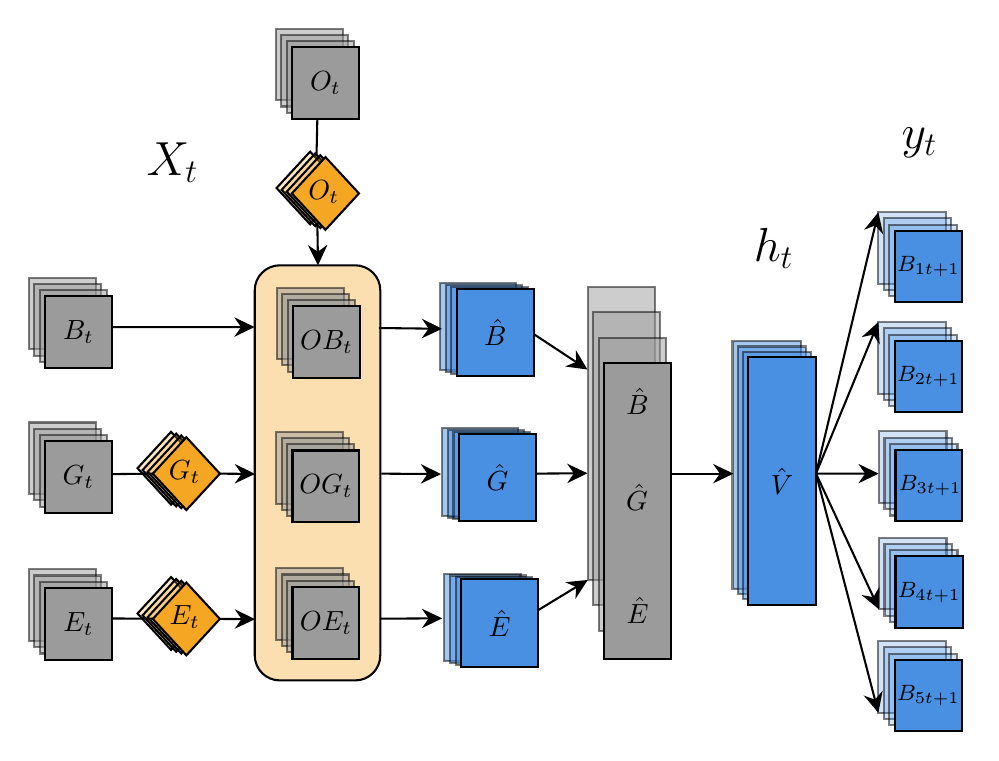
\begin{tikzpicture}[x=0.75pt,y=0.75pt,yscale=-1,xscale=1]
    %uncomment if require: \path (0,1033); %set diagram left start at 0, and has height of 1033
    
    %Rounded Rect [id:dp15650356150345013] 
    \draw  [fill={rgb, 255:red, 245; green, 166; blue, 35 }  ,fill opacity=0.36 ] (219.9,142.15) .. controls (219.9,135.47) and (225.32,130.05) .. (232,130.05) -- (268.3,130.05) .. controls (274.98,130.05) and (280.4,135.47) .. (280.4,142.15) -- (280.4,317.95) .. controls (280.4,324.63) and (274.98,330.05) .. (268.3,330.05) -- (232,330.05) .. controls (225.32,330.05) and (219.9,324.63) .. (219.9,317.95) -- cycle ;
    %Straight Lines [id:da409284418173784] 
    \draw    (250.06,109.76) -- (250.35,127.05) ;
    \draw [shift={(250.4,130.05)}, rotate = 269.03] [fill={rgb, 255:red, 0; green, 0; blue, 0 }  ][line width=0.08]  [draw opacity=0] (9.82,-4.72) -- (0,0) -- (9.82,4.72) -- (6.52,0) -- cycle    ;
    %Shape: Rectangle [id:dp7034345660290355] 
    \draw  [color={rgb, 255:red, 0; green, 0; blue, 0 }  ,draw opacity=0.5 ][fill={rgb, 255:red, 155; green, 155; blue, 155 }  ,fill opacity=0.5 ] (111.01,276.53) -- (143.26,276.53) -- (143.26,311.05) -- (111.01,311.05) -- cycle ;
    %Shape: Rectangle [id:dp22118233628007533] 
    \draw  [color={rgb, 255:red, 0; green, 0; blue, 0 }  ,draw opacity=0.5 ][fill={rgb, 255:red, 155; green, 155; blue, 155 }  ,fill opacity=0.5 ] (113.63,279.51) -- (145.88,279.51) -- (145.88,314.03) -- (113.63,314.03) -- cycle ;
    %Shape: Rectangle [id:dp24867768000931467] 
    \draw  [color={rgb, 255:red, 0; green, 0; blue, 0 }  ,draw opacity=0.5 ][fill={rgb, 255:red, 155; green, 155; blue, 155 }  ,fill opacity=0.5 ] (116.27,282.56) -- (148.53,282.56) -- (148.53,317.08) -- (116.27,317.08) -- cycle ;
    %Shape: Rectangle [id:dp124905579804508] 
    \draw  [fill={rgb, 255:red, 155; green, 155; blue, 155 }  ,fill opacity=1 ] (118.86,285.5) -- (151.11,285.5) -- (151.11,320.02) -- (118.86,320.02) -- cycle ;
    %Straight Lines [id:da8537240673366849] 
    \draw    (250.06,59.86) -- (249.67,77.43) ;
    %Shape: Rectangle [id:dp1958055080757597] 
    \draw  [color={rgb, 255:red, 0; green, 0; blue, 0 }  ,draw opacity=0.5 ][fill={rgb, 255:red, 74; green, 144; blue, 226 }  ,fill opacity=0.25 ] (520.36,157.39) -- (552.87,157.39) -- (552.87,191.9) -- (520.36,191.9) -- cycle ;
    %Shape: Rectangle [id:dp20825701586292622] 
    \draw  [color={rgb, 255:red, 0; green, 0; blue, 0 }  ,draw opacity=0.5 ][fill={rgb, 255:red, 74; green, 144; blue, 226 }  ,fill opacity=0.25 ] (523,160.37) -- (555.51,160.37) -- (555.51,194.88) -- (523,194.88) -- cycle ;
    %Shape: Rectangle [id:dp6709034910590727] 
    \draw  [color={rgb, 255:red, 0; green, 0; blue, 0 }  ,draw opacity=0.5 ][fill={rgb, 255:red, 74; green, 144; blue, 226 }  ,fill opacity=0.25 ] (525.67,163.42) -- (558.17,163.42) -- (558.17,197.93) -- (525.67,197.93) -- cycle ;
    %Shape: Rectangle [id:dp943426610209301] 
    \draw  [fill={rgb, 255:red, 74; green, 144; blue, 226 }  ,fill opacity=1 ] (528.28,166.36) -- (560.78,166.36) -- (560.78,200.87) -- (528.28,200.87) -- cycle ;
    %Shape: Rectangle [id:dp9270730461824767] 
    \draw  [color={rgb, 255:red, 0; green, 0; blue, 0 }  ,draw opacity=0.5 ][fill={rgb, 255:red, 74; green, 144; blue, 226 }  ,fill opacity=0.25 ] (520.69,210.06) -- (553.2,210.06) -- (553.2,244.56) -- (520.69,244.56) -- cycle ;
    %Shape: Rectangle [id:dp9671567967621458] 
    \draw  [color={rgb, 255:red, 0; green, 0; blue, 0 }  ,draw opacity=0.5 ][fill={rgb, 255:red, 74; green, 144; blue, 226 }  ,fill opacity=0.25 ] (523.33,213.04) -- (555.84,213.04) -- (555.84,247.54) -- (523.33,247.54) -- cycle ;
    %Shape: Rectangle [id:dp6567850092606636] 
    \draw  [color={rgb, 255:red, 0; green, 0; blue, 0 }  ,draw opacity=0.5 ][fill={rgb, 255:red, 74; green, 144; blue, 226 }  ,fill opacity=0.25 ] (526,216.09) -- (558.5,216.09) -- (558.5,250.6) -- (526,250.6) -- cycle ;
    %Shape: Rectangle [id:dp9307909660529495] 
    \draw  [fill={rgb, 255:red, 74; green, 144; blue, 226 }  ,fill opacity=1 ] (528.62,219.02) -- (560.84,219.02) -- (560.84,253.22) -- (528.62,253.22) -- cycle ;
    %Shape: Rectangle [id:dp2956426995252315] 
    \draw  [color={rgb, 255:red, 0; green, 0; blue, 0 }  ,draw opacity=0.5 ][fill={rgb, 255:red, 74; green, 144; blue, 226 }  ,fill opacity=0.25 ] (520.36,311.11) -- (552.87,311.11) -- (552.87,345.62) -- (520.36,345.62) -- cycle ;
    %Shape: Rectangle [id:dp9676718309145981] 
    \draw  [color={rgb, 255:red, 0; green, 0; blue, 0 }  ,draw opacity=0.5 ][fill={rgb, 255:red, 74; green, 144; blue, 226 }  ,fill opacity=0.25 ] (523,314.09) -- (555.51,314.09) -- (555.51,348.6) -- (523,348.6) -- cycle ;
    %Shape: Rectangle [id:dp3802447939611997] 
    \draw  [color={rgb, 255:red, 0; green, 0; blue, 0 }  ,draw opacity=0.5 ][fill={rgb, 255:red, 74; green, 144; blue, 226 }  ,fill opacity=0.25 ] (525.67,317.14) -- (558.17,317.14) -- (558.17,351.65) -- (525.67,351.65) -- cycle ;
    %Shape: Rectangle [id:dp2655409211543931] 
    \draw  [fill={rgb, 255:red, 74; green, 144; blue, 226 }  ,fill opacity=1 ] (528.28,320.08) -- (560.78,320.08) -- (560.78,354.59) -- (528.28,354.59) -- cycle ;
    %Shape: Rectangle [id:dp4040153422296009] 
    \draw  [color={rgb, 255:red, 0; green, 0; blue, 0 }  ,draw opacity=0.5 ][fill={rgb, 255:red, 74; green, 144; blue, 226 }  ,fill opacity=0.25 ] (520.69,261.32) -- (553.2,261.32) -- (553.2,295.83) -- (520.69,295.83) -- cycle ;
    %Shape: Rectangle [id:dp7066102537923638] 
    \draw  [color={rgb, 255:red, 0; green, 0; blue, 0 }  ,draw opacity=0.5 ][fill={rgb, 255:red, 74; green, 144; blue, 226 }  ,fill opacity=0.25 ] (523.33,264.3) -- (555.84,264.3) -- (555.84,298.81) -- (523.33,298.81) -- cycle ;
    %Shape: Rectangle [id:dp46050637304135866] 
    \draw  [color={rgb, 255:red, 0; green, 0; blue, 0 }  ,draw opacity=0.5 ][fill={rgb, 255:red, 74; green, 144; blue, 226 }  ,fill opacity=0.25 ] (526,267.35) -- (558.5,267.35) -- (558.5,301.86) -- (526,301.86) -- cycle ;
    %Shape: Rectangle [id:dp2033829273595421] 
    \draw  [fill={rgb, 255:red, 74; green, 144; blue, 226 }  ,fill opacity=1 ] (528.61,270.29) -- (561.11,270.29) -- (561.11,304.8) -- (528.61,304.8) -- cycle ;
    %Shape: Rectangle [id:dp19424752965877823] 
    \draw  [color={rgb, 255:red, 0; green, 0; blue, 0 }  ,draw opacity=0.5 ][fill={rgb, 255:red, 74; green, 144; blue, 226 }  ,fill opacity=0.25 ] (520.36,104.48) -- (552.87,104.48) -- (552.87,138.98) -- (520.36,138.98) -- cycle ;
    %Shape: Rectangle [id:dp6987771152166413] 
    \draw  [color={rgb, 255:red, 0; green, 0; blue, 0 }  ,draw opacity=0.5 ][fill={rgb, 255:red, 74; green, 144; blue, 226 }  ,fill opacity=0.25 ] (523,107.46) -- (555.51,107.46) -- (555.51,141.96) -- (523,141.96) -- cycle ;
    %Shape: Rectangle [id:dp12765942569283661] 
    \draw  [color={rgb, 255:red, 0; green, 0; blue, 0 }  ,draw opacity=0.5 ][fill={rgb, 255:red, 74; green, 144; blue, 226 }  ,fill opacity=0.25 ] (525.67,110.51) -- (558.17,110.51) -- (558.17,145.01) -- (525.67,145.01) -- cycle ;
    %Shape: Rectangle [id:dp16248810139444148] 
    \draw  [fill={rgb, 255:red, 74; green, 144; blue, 226 }  ,fill opacity=1 ] (528.28,113.44) -- (560.78,113.44) -- (560.78,147.95) -- (528.28,147.95) -- cycle ;
    %Shape: Rectangle [id:dp7988673729176894] 
    \draw  [color={rgb, 255:red, 0; green, 0; blue, 0 }  ,draw opacity=0.5 ][fill={rgb, 255:red, 155; green, 155; blue, 155 }  ,fill opacity=0.5 ] (111.01,205.77) -- (143.26,205.77) -- (143.26,240.29) -- (111.01,240.29) -- cycle ;
    %Shape: Rectangle [id:dp9623129937085917] 
    \draw  [color={rgb, 255:red, 0; green, 0; blue, 0 }  ,draw opacity=0.5 ][fill={rgb, 255:red, 155; green, 155; blue, 155 }  ,fill opacity=0.5 ] (113.63,208.75) -- (145.88,208.75) -- (145.88,243.27) -- (113.63,243.27) -- cycle ;
    %Shape: Rectangle [id:dp429379441325212] 
    \draw  [color={rgb, 255:red, 0; green, 0; blue, 0 }  ,draw opacity=0.5 ][fill={rgb, 255:red, 155; green, 155; blue, 155 }  ,fill opacity=0.5 ] (116.27,211.8) -- (148.53,211.8) -- (148.53,246.32) -- (116.27,246.32) -- cycle ;
    %Shape: Rectangle [id:dp9493890675957639] 
    \draw  [fill={rgb, 255:red, 155; green, 155; blue, 155 }  ,fill opacity=1 ] (118.86,214.74) -- (151.11,214.74) -- (151.11,249.26) -- (118.86,249.26) -- cycle ;
    %Straight Lines [id:da0399560958706785] 
    \draw [fill={rgb, 255:red, 155; green, 155; blue, 155 }  ,fill opacity=1 ]   (150.09,159.83) -- (216.85,159.8) ;
    \draw [shift={(219.85,159.8)}, rotate = 179.98] [fill={rgb, 255:red, 0; green, 0; blue, 0 }  ][line width=0.08]  [draw opacity=0] (9.82,-4.72) -- (0,0) -- (9.82,4.72) -- (6.52,0) -- cycle    ;
    %Shape: Rectangle [id:dp3393145890474042] 
    \draw  [color={rgb, 255:red, 0; green, 0; blue, 0 }  ,draw opacity=0.5 ][fill={rgb, 255:red, 155; green, 155; blue, 155 }  ,fill opacity=0.5 ] (111.01,136.06) -- (143.26,136.06) -- (143.26,170.57) -- (111.01,170.57) -- cycle ;
    %Shape: Rectangle [id:dp27631704382885136] 
    \draw  [color={rgb, 255:red, 0; green, 0; blue, 0 }  ,draw opacity=0.5 ][fill={rgb, 255:red, 155; green, 155; blue, 155 }  ,fill opacity=0.5 ] (113.63,139.04) -- (145.88,139.04) -- (145.88,173.55) -- (113.63,173.55) -- cycle ;
    %Shape: Rectangle [id:dp8553441662393909] 
    \draw  [color={rgb, 255:red, 0; green, 0; blue, 0 }  ,draw opacity=0.5 ][fill={rgb, 255:red, 155; green, 155; blue, 155 }  ,fill opacity=0.5 ] (116.27,142.09) -- (148.53,142.09) -- (148.53,176.61) -- (116.27,176.61) -- cycle ;
    %Shape: Rectangle [id:dp4571491350911555] 
    \draw  [fill={rgb, 255:red, 155; green, 155; blue, 155 }  ,fill opacity=1 ] (118.86,145.03) -- (151.11,145.03) -- (151.11,179.54) -- (118.86,179.54) -- cycle ;
    %Shape: Diamond [id:dp42134346339770745] 
    \draw  [fill={rgb, 255:red, 245; green, 166; blue, 35 }  ,fill opacity=0.25 ] (179.6,210.28) -- (195.77,227.81) -- (179.6,245.33) -- (163.43,227.81) -- cycle ;
    %Shape: Diamond [id:dp8160874162123375] 
    \draw  [fill={rgb, 255:red, 245; green, 166; blue, 35 }  ,fill opacity=0.25 ] (182.05,211.16) -- (198.22,228.68) -- (182.05,246.2) -- (165.89,228.68) -- cycle ;
    %Shape: Diamond [id:dp05986250472128074] 
    \draw  [fill={rgb, 255:red, 245; green, 166; blue, 35 }  ,fill opacity=0.25 ] (184.51,212.04) -- (200.68,229.56) -- (184.51,247.08) -- (168.34,229.56) -- cycle ;
    %Shape: Diamond [id:dp6831575900746938] 
    \draw  [fill={rgb, 255:red, 245; green, 166; blue, 35 }  ,fill opacity=1 ] (186.97,212.91) -- (203.13,230.43) -- (186.97,247.96) -- (170.8,230.43) -- cycle ;
    %Straight Lines [id:da3169233008507637] 
    \draw    (151.46,230.66) -- (170.8,230.43) ;
    %Shape: Diamond [id:dp08100159339963764] 
    \draw  [fill={rgb, 255:red, 245; green, 166; blue, 35 }  ,fill opacity=0.25 ] (179.6,280.28) -- (195.77,297.81) -- (179.6,315.33) -- (163.43,297.81) -- cycle ;
    %Shape: Diamond [id:dp6545409040088919] 
    \draw  [fill={rgb, 255:red, 245; green, 166; blue, 35 }  ,fill opacity=0.25 ] (182.05,281.16) -- (198.22,298.68) -- (182.05,316.2) -- (165.89,298.68) -- cycle ;
    %Shape: Diamond [id:dp22008618792927115] 
    \draw  [fill={rgb, 255:red, 245; green, 166; blue, 35 }  ,fill opacity=0.25 ] (184.51,282.04) -- (200.68,299.56) -- (184.51,317.08) -- (168.34,299.56) -- cycle ;
    %Shape: Diamond [id:dp6216162169932065] 
    \draw  [fill={rgb, 255:red, 245; green, 166; blue, 35 }  ,fill opacity=1 ] (186.97,282.91) -- (203.13,300.43) -- (186.97,317.96) -- (170.8,300.43) -- cycle ;
    %Straight Lines [id:da6348314705630924] 
    \draw    (203.13,300.43) -- (217.07,300.51) ;
    \draw [shift={(220.07,300.53)}, rotate = 180.32] [fill={rgb, 255:red, 0; green, 0; blue, 0 }  ][line width=0.08]  [draw opacity=0] (9.82,-4.72) -- (0,0) -- (9.82,4.72) -- (6.52,0) -- cycle    ;
    %Straight Lines [id:da29443986089740126] 
    \draw    (150.89,300.2) -- (170.89,300.31) ;
    %Straight Lines [id:da7037674707293678] 
    \draw [fill={rgb, 255:red, 155; green, 155; blue, 155 }  ,fill opacity=1 ]   (279.77,160.26) -- (307.2,160.6) ;
    \draw [shift={(310.2,160.63)}, rotate = 180.71] [fill={rgb, 255:red, 0; green, 0; blue, 0 }  ][line width=0.08]  [draw opacity=0] (9.82,-4.72) -- (0,0) -- (9.82,4.72) -- (6.52,0) -- cycle    ;
    %Straight Lines [id:da04725287763752273] 
    \draw [fill={rgb, 255:red, 155; green, 155; blue, 155 }  ,fill opacity=1 ]   (350.2,160.45) -- (377.7,178.6) ;
    \draw [shift={(380.2,180.25)}, rotate = 213.42] [fill={rgb, 255:red, 0; green, 0; blue, 0 }  ][line width=0.08]  [draw opacity=0] (9.82,-4.72) -- (0,0) -- (9.82,4.72) -- (6.52,0) -- cycle    ;
    %Straight Lines [id:da6945773359077246] 
    \draw    (203.13,230.43) -- (217.07,230.54) ;
    \draw [shift={(220.07,230.56)}, rotate = 180.44] [fill={rgb, 255:red, 0; green, 0; blue, 0 }  ][line width=0.08]  [draw opacity=0] (9.82,-4.72) -- (0,0) -- (9.82,4.72) -- (6.52,0) -- cycle    ;
    %Straight Lines [id:da6273046628189572] 
    \draw [fill={rgb, 255:red, 155; green, 155; blue, 155 }  ,fill opacity=1 ]   (280.91,230.43) -- (306.7,230.61) ;
    \draw [shift={(309.7,230.63)}, rotate = 180.41] [fill={rgb, 255:red, 0; green, 0; blue, 0 }  ][line width=0.08]  [draw opacity=0] (9.82,-4.72) -- (0,0) -- (9.82,4.72) -- (6.52,0) -- cycle    ;
    %Straight Lines [id:da5724582303552335] 
    \draw [fill={rgb, 255:red, 155; green, 155; blue, 155 }  ,fill opacity=1 ]   (280.63,300.31) -- (307.2,300.15) ;
    \draw [shift={(310.2,300.13)}, rotate = 179.65] [fill={rgb, 255:red, 0; green, 0; blue, 0 }  ][line width=0.08]  [draw opacity=0] (9.82,-4.72) -- (0,0) -- (9.82,4.72) -- (6.52,0) -- cycle    ;
    %Shape: Rectangle [id:dp53907172122875] 
    \draw  [color={rgb, 255:red, 0; green, 0; blue, 0 }  ,draw opacity=0.5 ][fill={rgb, 255:red, 155; green, 155; blue, 155 }  ,fill opacity=0.5 ] (230.01,16.06) -- (262.26,16.06) -- (262.26,50.57) -- (230.01,50.57) -- cycle ;
    %Shape: Rectangle [id:dp009192212091793661] 
    \draw  [color={rgb, 255:red, 0; green, 0; blue, 0 }  ,draw opacity=0.5 ][fill={rgb, 255:red, 155; green, 155; blue, 155 }  ,fill opacity=0.5 ] (232.63,19.04) -- (264.88,19.04) -- (264.88,53.55) -- (232.63,53.55) -- cycle ;
    %Shape: Rectangle [id:dp10982806096562447] 
    \draw  [color={rgb, 255:red, 0; green, 0; blue, 0 }  ,draw opacity=0.5 ][fill={rgb, 255:red, 155; green, 155; blue, 155 }  ,fill opacity=0.5 ] (235.27,22.09) -- (267.53,22.09) -- (267.53,56.61) -- (235.27,56.61) -- cycle ;
    %Shape: Rectangle [id:dp024787601372134982] 
    \draw  [fill={rgb, 255:red, 155; green, 155; blue, 155 }  ,fill opacity=1 ] (237.86,25.03) -- (270.11,25.03) -- (270.11,59.54) -- (237.86,59.54) -- cycle ;
    %Shape: Rectangle [id:dp9022114030928725] 
    \draw  [color={rgb, 255:red, 0; green, 0; blue, 0 }  ,draw opacity=0.5 ][fill={rgb, 255:red, 155; green, 155; blue, 155 }  ,fill opacity=0.5 ] (380.34,140.45) -- (412.6,140.45) -- (412.6,281.66) -- (380.34,281.66) -- cycle ;
    %Shape: Rectangle [id:dp9877830883323443] 
    \draw  [color={rgb, 255:red, 0; green, 0; blue, 0 }  ,draw opacity=0.5 ][fill={rgb, 255:red, 155; green, 155; blue, 155 }  ,fill opacity=0.5 ] (382.96,152.64) -- (415.22,152.64) -- (415.22,293.84) -- (382.96,293.84) -- cycle ;
    %Shape: Rectangle [id:dp8814167498359042] 
    \draw  [color={rgb, 255:red, 0; green, 0; blue, 0 }  ,draw opacity=0.5 ][fill={rgb, 255:red, 155; green, 155; blue, 155 }  ,fill opacity=0.5 ] (385.61,165.13) -- (417.86,165.13) -- (417.86,306.34) -- (385.61,306.34) -- cycle ;
    %Shape: Rectangle [id:dp5289911737134959] 
    \draw  [fill={rgb, 255:red, 155; green, 155; blue, 155 }  ,fill opacity=1 ] (388.19,177.14) -- (420.45,177.14) -- (420.45,319.53) -- (388.19,319.53) -- cycle ;
    %Shape: Rectangle [id:dp8149328215662492] 
    \draw  [color={rgb, 255:red, 0; green, 0; blue, 0 }  ,draw opacity=0.5 ][fill={rgb, 255:red, 155; green, 155; blue, 155 }  ,fill opacity=0.5 ] (230.51,140.77) -- (262.76,140.77) -- (262.76,175.29) -- (230.51,175.29) -- cycle ;
    %Shape: Rectangle [id:dp45921305478843055] 
    \draw  [color={rgb, 255:red, 0; green, 0; blue, 0 }  ,draw opacity=0.5 ][fill={rgb, 255:red, 155; green, 155; blue, 155 }  ,fill opacity=0.5 ] (233.13,143.75) -- (265.38,143.75) -- (265.38,178.27) -- (233.13,178.27) -- cycle ;
    %Shape: Rectangle [id:dp6228279530655318] 
    \draw  [color={rgb, 255:red, 0; green, 0; blue, 0 }  ,draw opacity=0.5 ][fill={rgb, 255:red, 155; green, 155; blue, 155 }  ,fill opacity=0.5 ] (235.77,146.8) -- (268.03,146.8) -- (268.03,181.32) -- (235.77,181.32) -- cycle ;
    %Shape: Rectangle [id:dp3598797805540589] 
    \draw  [fill={rgb, 255:red, 155; green, 155; blue, 155 }  ,fill opacity=1 ] (238.36,149.74) -- (270.61,149.74) -- (270.61,184.26) -- (238.36,184.26) -- cycle ;
    %Shape: Rectangle [id:dp9661891091990619] 
    \draw  [color={rgb, 255:red, 0; green, 0; blue, 0 }  ,draw opacity=0.5 ][fill={rgb, 255:red, 155; green, 155; blue, 155 }  ,fill opacity=0.5 ] (230.26,210.32) -- (262.51,210.32) -- (262.51,244.84) -- (230.26,244.84) -- cycle ;
    %Shape: Rectangle [id:dp690231151268716] 
    \draw  [color={rgb, 255:red, 0; green, 0; blue, 0 }  ,draw opacity=0.5 ][fill={rgb, 255:red, 155; green, 155; blue, 155 }  ,fill opacity=0.5 ] (232.88,213.3) -- (265.13,213.3) -- (265.13,247.82) -- (232.88,247.82) -- cycle ;
    %Shape: Rectangle [id:dp48804619093484347] 
    \draw  [color={rgb, 255:red, 0; green, 0; blue, 0 }  ,draw opacity=0.5 ][fill={rgb, 255:red, 155; green, 155; blue, 155 }  ,fill opacity=0.5 ] (235.52,216.35) -- (267.78,216.35) -- (267.78,250.87) -- (235.52,250.87) -- cycle ;
    %Shape: Rectangle [id:dp22992925838286216] 
    \draw  [fill={rgb, 255:red, 155; green, 155; blue, 155 }  ,fill opacity=1 ] (238.11,219.29) -- (270.36,219.29) -- (270.36,253.81) -- (238.11,253.81) -- cycle ;
    %Shape: Rectangle [id:dp29039742489844134] 
    \draw  [color={rgb, 255:red, 0; green, 0; blue, 0 }  ,draw opacity=0.5 ][fill={rgb, 255:red, 155; green, 155; blue, 155 }  ,fill opacity=0.5 ] (230.26,276.02) -- (262.51,276.02) -- (262.51,310.54) -- (230.26,310.54) -- cycle ;
    %Shape: Rectangle [id:dp42091335353816794] 
    \draw  [color={rgb, 255:red, 0; green, 0; blue, 0 }  ,draw opacity=0.5 ][fill={rgb, 255:red, 155; green, 155; blue, 155 }  ,fill opacity=0.5 ] (232.88,279) -- (265.13,279) -- (265.13,313.52) -- (232.88,313.52) -- cycle ;
    %Shape: Rectangle [id:dp9855473947081604] 
    \draw  [color={rgb, 255:red, 0; green, 0; blue, 0 }  ,draw opacity=0.5 ][fill={rgb, 255:red, 155; green, 155; blue, 155 }  ,fill opacity=0.5 ] (235.52,282.05) -- (267.78,282.05) -- (267.78,316.57) -- (235.52,316.57) -- cycle ;
    %Shape: Rectangle [id:dp434232717458334] 
    \draw  [fill={rgb, 255:red, 155; green, 155; blue, 155 }  ,fill opacity=1 ] (238.11,284.99) -- (270.36,284.99) -- (270.36,319.51) -- (238.11,319.51) -- cycle ;
    %Shape: Diamond [id:dp30872576312410427] 
    \draw  [fill={rgb, 255:red, 245; green, 166; blue, 35 }  ,fill opacity=0.25 ] (246.6,75.28) -- (262.77,92.81) -- (246.6,110.33) -- (230.43,92.81) -- cycle ;
    %Shape: Diamond [id:dp6849972388912634] 
    \draw  [fill={rgb, 255:red, 245; green, 166; blue, 35 }  ,fill opacity=0.25 ] (249.05,76.16) -- (265.22,93.68) -- (249.05,111.2) -- (232.89,93.68) -- cycle ;
    %Shape: Diamond [id:dp857485897511279] 
    \draw  [fill={rgb, 255:red, 245; green, 166; blue, 35 }  ,fill opacity=0.25 ] (251.51,77.04) -- (267.68,94.56) -- (251.51,112.08) -- (235.34,94.56) -- cycle ;
    %Shape: Diamond [id:dp49326046176048577] 
    \draw  [fill={rgb, 255:red, 245; green, 166; blue, 35 }  ,fill opacity=1 ] (253.97,77.91) -- (270.13,95.43) -- (253.97,112.96) -- (237.8,95.43) -- cycle ;
    %Straight Lines [id:da9533396825264671] 
    \draw [fill={rgb, 255:red, 155; green, 155; blue, 155 }  ,fill opacity=1 ]   (349.2,230.45) -- (377.2,230.27) ;
    \draw [shift={(380.2,230.25)}, rotate = 179.63] [fill={rgb, 255:red, 0; green, 0; blue, 0 }  ][line width=0.08]  [draw opacity=0] (9.82,-4.72) -- (0,0) -- (9.82,4.72) -- (6.52,0) -- cycle    ;
    %Straight Lines [id:da46693829157920863] 
    \draw [fill={rgb, 255:red, 155; green, 155; blue, 155 }  ,fill opacity=1 ]   (350.4,299.88) -- (377.78,283.22) ;
    \draw [shift={(380.34,281.66)}, rotate = 148.68] [fill={rgb, 255:red, 0; green, 0; blue, 0 }  ][line width=0.08]  [draw opacity=0] (9.82,-4.72) -- (0,0) -- (9.82,4.72) -- (6.52,0) -- cycle    ;
    %Straight Lines [id:da9477168442608538] 
    \draw [fill={rgb, 255:red, 155; green, 155; blue, 155 }  ,fill opacity=1 ]   (421.09,230.43) -- (447.51,230.43) ;
    \draw [shift={(450.51,230.43)}, rotate = 180] [fill={rgb, 255:red, 0; green, 0; blue, 0 }  ][line width=0.08]  [draw opacity=0] (9.82,-4.72) -- (0,0) -- (9.82,4.72) -- (6.52,0) -- cycle    ;
    %Straight Lines [id:da17588566125157779] 
    \draw [fill={rgb, 255:red, 155; green, 155; blue, 155 }  ,fill opacity=1 ]   (490.32,230.39) -- (517.51,230.42) ;
    \draw [shift={(520.51,230.43)}, rotate = 180.08] [fill={rgb, 255:red, 0; green, 0; blue, 0 }  ][line width=0.08]  [draw opacity=0] (9.82,-4.72) -- (0,0) -- (9.82,4.72) -- (6.52,0) -- cycle    ;
    %Straight Lines [id:da990575471229112] 
    \draw [fill={rgb, 255:red, 155; green, 155; blue, 155 }  ,fill opacity=1 ]   (490.32,230.39) -- (519.43,293.11) ;
    \draw [shift={(520.69,295.83)}, rotate = 245.1] [fill={rgb, 255:red, 0; green, 0; blue, 0 }  ][line width=0.08]  [draw opacity=0] (9.82,-4.72) -- (0,0) -- (9.82,4.72) -- (6.52,0) -- cycle    ;
    %Straight Lines [id:da11726542356327818] 
    \draw [fill={rgb, 255:red, 155; green, 155; blue, 155 }  ,fill opacity=1 ]   (490.32,230.39) -- (519.61,342.72) ;
    \draw [shift={(520.36,345.62)}, rotate = 255.39] [fill={rgb, 255:red, 0; green, 0; blue, 0 }  ][line width=0.08]  [draw opacity=0] (9.82,-4.72) -- (0,0) -- (9.82,4.72) -- (6.52,0) -- cycle    ;
    %Straight Lines [id:da6006783627611112] 
    \draw [fill={rgb, 255:red, 155; green, 155; blue, 155 }  ,fill opacity=1 ]   (490.32,230.39) -- (519.22,160.17) ;
    \draw [shift={(520.36,157.39)}, rotate = 112.37] [fill={rgb, 255:red, 0; green, 0; blue, 0 }  ][line width=0.08]  [draw opacity=0] (9.82,-4.72) -- (0,0) -- (9.82,4.72) -- (6.52,0) -- cycle    ;
    %Straight Lines [id:da16067428057688105] 
    \draw [fill={rgb, 255:red, 155; green, 155; blue, 155 }  ,fill opacity=1 ]   (490.32,230.39) -- (519.67,107.4) ;
    \draw [shift={(520.36,104.48)}, rotate = 103.42] [fill={rgb, 255:red, 0; green, 0; blue, 0 }  ][line width=0.08]  [draw opacity=0] (9.82,-4.72) -- (0,0) -- (9.82,4.72) -- (6.52,0) -- cycle    ;
    %Shape: Rectangle [id:dp04777231109494484] 
    \draw  [color={rgb, 255:red, 0; green, 0; blue, 0 }  ,draw opacity=0.5 ][fill={rgb, 255:red, 74; green, 144; blue, 226 }  ,fill opacity=0.5 ] (309.1,138.6) -- (345.95,138.6) -- (345.95,180.65) -- (309.1,180.65) -- cycle ;
    %Shape: Rectangle [id:dp7558311796324689] 
    \draw  [color={rgb, 255:red, 0; green, 0; blue, 0 }  ,draw opacity=0.5 ][fill={rgb, 255:red, 74; green, 144; blue, 226 }  ,fill opacity=0.5 ] (311.88,139.51) -- (348.73,139.51) -- (348.73,181.56) -- (311.88,181.56) -- cycle ;
    %Shape: Rectangle [id:dp02297715036875614] 
    \draw  [color={rgb, 255:red, 0; green, 0; blue, 0 }  ,draw opacity=0.5 ][fill={rgb, 255:red, 74; green, 144; blue, 226 }  ,fill opacity=0.5 ] (314.67,140.42) -- (351.51,140.42) -- (351.51,182.46) -- (314.67,182.46) -- cycle ;
    %Shape: Rectangle [id:dp7483619990673073] 
    \draw  [fill={rgb, 255:red, 74; green, 144; blue, 226 }  ,fill opacity=1 ] (317.45,141.33) -- (354.29,141.33) -- (354.29,183.37) -- (317.45,183.37) -- cycle ;
    %Shape: Rectangle [id:dp8163589302848298] 
    \draw  [color={rgb, 255:red, 0; green, 0; blue, 0 }  ,draw opacity=0.5 ][fill={rgb, 255:red, 74; green, 144; blue, 226 }  ,fill opacity=0.5 ] (450.1,166.6) -- (482.87,166.6) -- (482.87,285.87) -- (450.1,285.87) -- cycle ;
    %Shape: Rectangle [id:dp13561622734198409] 
    \draw  [color={rgb, 255:red, 0; green, 0; blue, 0 }  ,draw opacity=0.5 ][fill={rgb, 255:red, 74; green, 144; blue, 226 }  ,fill opacity=0.5 ] (452.57,169.18) -- (485.34,169.18) -- (485.34,288.44) -- (452.57,288.44) -- cycle ;
    %Shape: Rectangle [id:dp028266783786446537] 
    \draw  [color={rgb, 255:red, 0; green, 0; blue, 0 }  ,draw opacity=0.5 ][fill={rgb, 255:red, 74; green, 144; blue, 226 }  ,fill opacity=0.5 ] (455.05,171.76) -- (487.82,171.76) -- (487.82,291.02) -- (455.05,291.02) -- cycle ;
    %Shape: Rectangle [id:dp501556684499422] 
    \draw  [fill={rgb, 255:red, 74; green, 144; blue, 226 }  ,fill opacity=1 ] (457.52,174.33) -- (490.29,174.33) -- (490.29,293.6) -- (457.52,293.6) -- cycle ;
    
    %Shape: Rectangle [id:dp3431119253458095] 
    \draw  [color={rgb, 255:red, 0; green, 0; blue, 0 }  ,draw opacity=0.5 ][fill={rgb, 255:red, 74; green, 144; blue, 226 }  ,fill opacity=0.5 ] (310.1,208.6) -- (346.95,208.6) -- (346.95,250.65) -- (310.1,250.65) -- cycle ;
    %Shape: Rectangle [id:dp8294825257941912] 
    \draw  [color={rgb, 255:red, 0; green, 0; blue, 0 }  ,draw opacity=0.5 ][fill={rgb, 255:red, 74; green, 144; blue, 226 }  ,fill opacity=0.5 ] (312.88,209.51) -- (349.73,209.51) -- (349.73,251.56) -- (312.88,251.56) -- cycle ;
    %Shape: Rectangle [id:dp049289680132614255] 
    \draw  [color={rgb, 255:red, 0; green, 0; blue, 0 }  ,draw opacity=0.5 ][fill={rgb, 255:red, 74; green, 144; blue, 226 }  ,fill opacity=0.5 ] (315.67,210.42) -- (352.51,210.42) -- (352.51,252.46) -- (315.67,252.46) -- cycle ;
    %Shape: Rectangle [id:dp4657902939703581] 
    \draw  [fill={rgb, 255:red, 74; green, 144; blue, 226 }  ,fill opacity=1 ] (318.45,211.33) -- (355.29,211.33) -- (355.29,253.37) -- (318.45,253.37) -- cycle ;
    %Shape: Rectangle [id:dp8549615376830864] 
    \draw  [color={rgb, 255:red, 0; green, 0; blue, 0 }  ,draw opacity=0.5 ][fill={rgb, 255:red, 74; green, 144; blue, 226 }  ,fill opacity=0.5 ] (311.1,278.6) -- (347.95,278.6) -- (347.95,320.65) -- (311.1,320.65) -- cycle ;
    %Shape: Rectangle [id:dp07757251126817089] 
    \draw  [color={rgb, 255:red, 0; green, 0; blue, 0 }  ,draw opacity=0.5 ][fill={rgb, 255:red, 74; green, 144; blue, 226 }  ,fill opacity=0.5 ] (313.88,279.51) -- (350.73,279.51) -- (350.73,321.56) -- (313.88,321.56) -- cycle ;
    %Shape: Rectangle [id:dp9077595517238054] 
    \draw  [color={rgb, 255:red, 0; green, 0; blue, 0 }  ,draw opacity=0.5 ][fill={rgb, 255:red, 74; green, 144; blue, 226 }  ,fill opacity=0.5 ] (316.67,280.42) -- (353.51,280.42) -- (353.51,322.46) -- (316.67,322.46) -- cycle ;
    %Shape: Rectangle [id:dp2039123260975314] 
    \draw  [fill={rgb, 255:red, 74; green, 144; blue, 226 }  ,fill opacity=1 ] (319.45,281.33) -- (356.29,281.33) -- (356.29,323.37) -- (319.45,323.37) -- cycle ;
    
    % Text Node
    \draw (134.99,302.76) node  [font=\normalsize]  {$E_{t}$};
    % Text Node
    \draw (180.34,80.58) node  [font=\LARGE]  {$X_{t}$};
    % Text Node
    \draw (470.01,121.94) node  [font=\LARGE]  {$h_{t}$};
    % Text Node
    \draw (544.53,183.61) node  [font=\footnotesize]  {$B_{2t+1}$};
    % Text Node
    \draw (545.41,236.28) node  [font=\footnotesize]  {$B_{3t+1}$};
    % Text Node
    \draw (544.86,287.54) node  [font=\footnotesize]  {$B_{4t+1}$};
    % Text Node
    \draw (544.53,337.33) node  [font=\footnotesize]  {$B_{5t+1}$};
    % Text Node
    \draw (540.21,70.84) node  [font=\LARGE]  {$y_{t}$};
    % Text Node
    \draw (544.53,130.7) node  [font=\footnotesize]  {$B_{1t+1}$};
    % Text Node
    \draw (134.99,232) node  [font=\normalsize]  {$G_{t}$};
    % Text Node
    \draw (134.99,162.29) node  [font=\normalsize]  {$B_{t}$};
    % Text Node
    \draw (186.15,229.56) node  [font=\normalsize]  {$G_{t}$};
    % Text Node
    \draw (186.15,299.56) node  [font=\normalsize]  {$E_{t}$};
    % Text Node
    \draw (253.99,42.29) node  [font=\normalsize]  {$O_{t}$};
    % Text Node
    \draw (254.49,167) node  [font=\normalsize]  {$OB_{t}$};
    % Text Node
    \draw (254.24,236.55) node  [font=\normalsize]  {$OG_{t}$};
    % Text Node
    \draw (254.24,302.25) node  [font=\normalsize]  {$OE_{t}$};
    % Text Node
    \draw (253.15,94.56) node  [font=\normalsize]  {$O_{t}$};
    % Text Node
    \draw (404.35,195.78) node  [font=\normalsize]  {$\hat{B}$};
    % Text Node
    \draw (404.07,242.06) node  [font=\normalsize]  {$\hat{G}$};
    % Text Node
    \draw (404.35,296.11) node  [font=\normalsize]  {$\hat{E}$};
    % Text Node
    \draw (473.91,233.97) node  [font=\normalsize]  {$\hat{V}$};
    % Text Node
    \draw (335.87,162.35) node  [font=\normalsize]  {$\hat{B}$};
    % Text Node
    \draw (336.87,232.35) node  [font=\normalsize]  {$\hat{G}$};
    % Text Node
    \draw (337.87,302.35) node  [font=\normalsize]  {$\hat{E}$};
    
    
    \end{tikzpicture}



\end{adjustbox}
\end{center}
\caption[\textbf{The environment-event time distributed multi layer perceptron architecture}]{Blue and orange shapes represent respectively feedforward and embedding operations. Gray shapes indicate operations with no learnable parameters, such as tensor instantiation and concatenation. Stacked, transparent colouring indicates tensors with a sequential structure. Straight arrows refer to the presence of feed-forward information flow. All the feedforward operations are time distributed.}
\label{fig: mlp_3}
\end{figure}

\subsection{Data}
\label{data_3}
In order to validate the architecture presented in section \ref{model_architecture_3}, we leveraged a dataset with similar characteristics to the one used in section \ref{data_2}. Despite still relying on gameplay data provided by our partner company, \textit{Square Enix Ltd.}, we had to drop one of the title (Hitman Sniper, hms) used in the previous stages of the model building process, as it was discontinued. As a replacement we decided to include data from a new open world action role-play game with cooperative multiplayer characteristics (Outriders, outr). 

The dataset contained entries from 2,805,952 individuals, evenly distributed across the six games, and randomly sampled from all users who played the games between their respective release date and January 2021. The reason for considering a reduced number of individuals in this stage of the model building process was mostly technical. The model outlined in section \ref{model_architecture_3}, along with its variation presented in section \ref{competing_models_3}, required a consistently larger amount of information per individual, making the model tuning and comparison steps rather demanding given the the available hardware. All data were obtained and processed in compliance with the European Union's General Data Protection Regulation \cite{EUdataregulations2018}. 

\paragraph*{Defining the Behavioural Metrics and Targets}
The metric used for representing the behavioural manifestations of state transition dynamics, were the same 
of those used for validating the RNN architecture with only a small variation,  we modified the way the metric Session Activity was computed. We moved from the count of user initiated gameplay actions to the ratio of actions per minute. The reason was that from a correlation a analysis we realized that this metric was highly correlated with the metric Session Time.
\begin{table}[H] \centering
\caption{Description of Selected Telemetries}
\label{metricsdescription_3}
  \begin{tabularx}{\textwidth}{@{}lX@{}}
    \toprule
    \textbf{Metric}      & \textbf{Description}          \\ \midrule
    {Absence}    & Temporal distance between sessions (hours)  \\
    {Session Time}     & Overall session duration (minutes)       \\ 
    {Active Time}      & Percentage of Session Time actively playing  \\ 
    {Session Activity}    & Ratio of user initiated gameplay-related actions per minute in Session Time. E.g.\\ 
                & "Attack an enemy" is considered a valid\\ 
                & action while "Being attacked by an enemy" is not.\\
    {N°Sessions}    & Number of played sessions.\\ 
    {Object}    &  Game object identifier.  \\
    \bottomrule
  \end{tabularx}
\end{table}
Similarly to what was done for the RNN architecture, the target consisted of the lead-1 version of the behavioural metrics described in table \ref{metricsdescription_3}.

\paragraph*{Defining the Environmental and Game Events Covariates}
In order to represent the environmental covariates we simply decomposed the trigger identifier associated with the start of a game session (we point to section \ref{data_2} for a more detailed definition of what defines a game session). These identifier usually holds information on where and when an individual initiated the game activity and are used for mapping multiple game events triggered during the playing activity to a single session. It is worth noticing that all the trigger identifiers were logged in Central European Time (CEST), we decided to not perform any time zone conversion and simply include indicators of the geographical area from where the trigger was recorded. A description of the information extracted can be found in table \ref{metricsdescription_env_3}

\begin{table}[H] \centering
\caption{Description of Selected Environmental Telemetries}
\label{metricsdescription_env_3}
  \begin{tabularx}{\textwidth}{@{}lX@{}}
    \toprule
    \textbf{Metric}      & \textbf{Description}          \\ \midrule
    {Hour of the Day}    & Hour of the day in which the session started.  \\
    {Day of the Week}     & Day of the week in which the session started.       \\ 
    {Day of the Month}      & Day of the month in which the session started.\\ 
    {Month of the Year}    & Month of the year in which the session started. \\
    {Country Area}    & Broad indicator of the country area in which the session started. \\ 
    \bottomrule
  \end{tabularx}
\end{table}

For incorporating information on the game events we first individuated which were most representative of the core gameplay of each title (e.g., interacting with the menu was not considered a relevant event). Subsequently for each session we obtained a list of the unique events triggered within that session and their associated frequencies. It is important to note that this list could be empty in case an individual played a session without interacting with any of the selected core gameplay events. A description of the considered game events can be found in table \ref{metricsdescription_event_3}

\begin{table}[H] \centering
\caption{Description of Selected Game Events Telemetries}
\label{metricsdescription_event_3}
  \begin{tabularx}{\textwidth}{@{}lX@{}}
    \toprule
    \textbf{Metric}      & \textbf{Description}          \\ \midrule
    {Game Events Set}    & Set of in-game events that might occur in a session  \\
    {Game Events Frequency}     & Frequencies at which each game event occurred in a particular session       \\ 
    \bottomrule
  \end{tabularx}
\end{table}

The final dataset was composed of 13 columns and 28,804,987 rows. A table of descriptive statistics for the behavioural metrics can be found in \ref{game_description_33}.

\begin{table*}[h]
\centering
\caption{Descriptive Statistics of Considered Metrics and Games}
\label{game_description_33}
  \begin{tabularx}{\textwidth}{cccccccX}
  \toprule
  \multirow{2}{*}{\textbf{Game}} &
   \multirow{2}{*}{\textbf{\begin{tabular}[c]{@{}c@{}}Sample \\ Size\end{tabular}}} &
   \textbf{\begin{tabular}[c]{@{}c@{}}Number \\ of \\ Sessions\end{tabular}} &
   \textbf{\begin{tabular}[c]{@{}c@{}}Absence \\ (minutes)\end{tabular}} &
   \textbf{\begin{tabular}[c]{@{}c@{}}Session \\ Time\\ (minutes)\end{tabular}} &
   \textbf{\begin{tabular}[c]{@{}c@{}}Active \\ Time\\ (\% Session Time)\end{tabular}} &
   \textbf{\begin{tabular}[c]{@{}c@{}}Session \\ Activity\end{tabular}} &
   \multirow{2}{*}{\textbf{\begin{tabularx}{\textwidth}[X]{@{}c@{}} Type \end{tabularx}}} \\ \midrule
   &
    &
   \multicolumn{5}{c}{\textbf{\begin{tabular}[c]{@{}c@{}}(Median $\pm$ IQR)\end{tabular}}} &
    \\ \midrule
  \textbf{hmg} &
   452,386 &
   \begin{tabular}[c]{@{}c@{}}5 $\pm$ 6\end{tabular} &
   \begin{tabular}[c]{@{}c@{}}141$\pm$ 219\end{tabular} &
   \begin{tabular}[c]{@{}c@{}}12 $\pm$ 15 \end{tabular} &
   \begin{tabular}[c]{@{}c@{}}87 $\pm$  24 \end{tabular} &
   \begin{tabular}[c]{@{}c@{}}1.3 $\pm$  0.9\end{tabular} &
   \begin{tabular}[c]{@{}c@{}}Mobile\\ Strategy\end{tabular} \\
  \textbf{jc3} &
   491,329 &
   \begin{tabular}[c]{@{}c@{}}7 $\pm$ 7\end{tabular} &
   \begin{tabular}[c]{@{}c@{}}27 $\pm$ 365\end{tabular} &
   \begin{tabular}[c]{@{}c@{}}64 $\pm$ 143\end{tabular} &
   \begin{tabular}[c]{@{}c@{}}99 $\pm$ 1\end{tabular} &
   \begin{tabular}[c]{@{}c@{}}0.18 $\pm$ 0.22 \end{tabular} &
   \begin{tabular}[c]{@{}c@{}}Console\\ Action\\Open\\World\end{tabular} \\
  \textbf{jc4} &
   485,276 &
   \begin{tabular}[c]{@{}c@{}}6 $\pm$ 7\end{tabular} &
   \begin{tabular}[c]{@{}c@{}}31 $\pm$ 356\end{tabular} &
   \begin{tabular}[c]{@{}c@{}}59 $\pm$ 87\end{tabular} &
   \begin{tabular}[c]{@{}c@{}}82 $\pm$ 25\end{tabular} &
   \begin{tabular}[c]{@{}c@{}}0.28 $\pm$ 0.45\end{tabular} &
   \begin{tabular}[c]{@{}c@{}}Console\\ Action\\Open\\World\end{tabular} \\
  \textbf{lis} &
   483,783 &
   \begin{tabular}[c]{@{}c@{}}5 $\pm$ 6 \end{tabular} &
   \begin{tabular}[c]{@{}c@{}}70 $\pm$ 844\end{tabular} &
   \begin{tabular}[c]{@{}c@{}}64 $\pm$ 104\end{tabular} &
   \begin{tabular}[c]{@{}c@{}}78 $\pm$ 25\end{tabular} &
   \begin{tabular}[c]{@{}c@{}}0.5 $\pm$ 0.4\end{tabular} &
   \begin{tabular}[c]{@{}c@{}}Console\\ Graphic\\ Adventure\end{tabular} \\
  \textbf{lisbf} &
   431,355 &
   \begin{tabular}[c]{@{}c@{}}6 $\pm$ 6\end{tabular} &
   \begin{tabular}[c]{@{}c@{}}173  $\pm$ 574\end{tabular} &
   \begin{tabular}[c]{@{}c@{}}67 $\pm$ 87\end{tabular} &
   \begin{tabular}[c]{@{}c@{}}81 $\pm$ 26\end{tabular} &
   \begin{tabular}[c]{@{}c@{}}0.08 $\pm$ 0.15\end{tabular} &
   \begin{tabular}[c]{@{}c@{}}Console\\ Graphic\\ Adventure\end{tabular} \\
  \textbf{outr} &
   461,823 &
   \begin{tabular}[c]{@{}c@{}}7 $\pm$ 7\end{tabular} &
   \begin{tabular}[c]{@{}c@{}}47 $\pm$ 33\end{tabular} &
   \begin{tabular}[c]{@{}c@{}}64 $\pm$ 121\end{tabular} &
   \begin{tabular}[c]{@{}c@{}}88 $\pm$ 65\end{tabular} &
   \begin{tabular}[c]{@{}c@{}}0.02 $\pm$ 0.04\end{tabular} &
   \begin{tabular}[c]{@{}c@{}}Console\\ Action\\Open\\World\\Co-op\end{tabular} \\ \bottomrule
  \end{tabularx}
\end{table*}

\paragraph*{Data Preparation} When querying the data from the game servers, we relied on the usual permissive filtering strategy by excluding from the random sampling procedure individuals having at least one of the considered behavioural metrics over the game population's \nth{99} percentile. Data were re-arranged in the conventional format suitable for time series modelling and randomly split into a tuning (i.e., 10 \%) and validation set (i.e., 90 \%). 

Model fitting was again done using the same batching strategy presented in section \ref{model_architecture_2} with the only difference that the data generator had now to provide the model with multiple input: a single multidimensional array of shape $(N \times T \times 5)$ for the behavioural metrics, 5 separate of arrays of shape $(N \times T \times 1)$ for the environmental covariates and 2 separate arrays of shape $(N \times T \times 7)$ for the game events covariates. Since the number of game events could vary from session to session, we first individuated the maximum number of unique events triggered in a session for the the entire dataset (i.e. 7), and subsequently zero padded the multidimensional arrays accordingly.

The behavioural metrics were min-max scaled according to the same formula defined in equation \ref{min_max} while the categorical inputs (i.e. game object, environmental and game events covariates) were encoded ordinally.

\subsection{Model Tuning and Comparison}
\label{tuning_comparison_3}
Model tuning and comparison followed almost the exact same strategy employed for validating the RNN architecture with only few minor differences. Due to time constrains and hardware limitations we reduced the budget assigned to Hyperband from 40 to 20 epochs and limited the number of cross-validation folds to 8. 

The cross validation results, with collapsed and non-collapsed targets, were again analysed using a Linear Mixed-effects Model (LMM) with game object and time as random effects and model type as fixed effect (treatment coded with the RNN architecture as reference). In order to investigate the hypotheses outlined in \ref{model_architecture_3} we carried out post-hoc comparisons (i.e. t-tests with Bonferroni correction) on the coefficient estimated by the LMM model expecting the following inequalities: RNN Env $<$ RNN Even $<$ MLP $<$ RNN Env Even. Also in this case the ancillary analyses conducted within a Bayesian framework did not diverge substantially from the frequentist analyses, details and additional results are provided in Appendix \ref{dynamic_prediction_ancillary_perf}. 

All statistical analyses were conducted using the python library statsmodels \cite{seabold2010statsmodels}.  All the models were implemented using Tensorflow's high level API "Keras" \cite{tensorflow2015-whitepaper,chollet2015keras}. 

\subsection{Results}
\label{results_3}
Inspecting the results of the regression analysis on the collapsed targets (see Table \ref{model_comp_coll_game_33} and Figure \ref{model_comp_coll_33}) we can see how introducing environmental and game events covariates led to a modest but robust improvement in performance when compared with the RNN architecture. 

\begin{figure}[h]
\centering
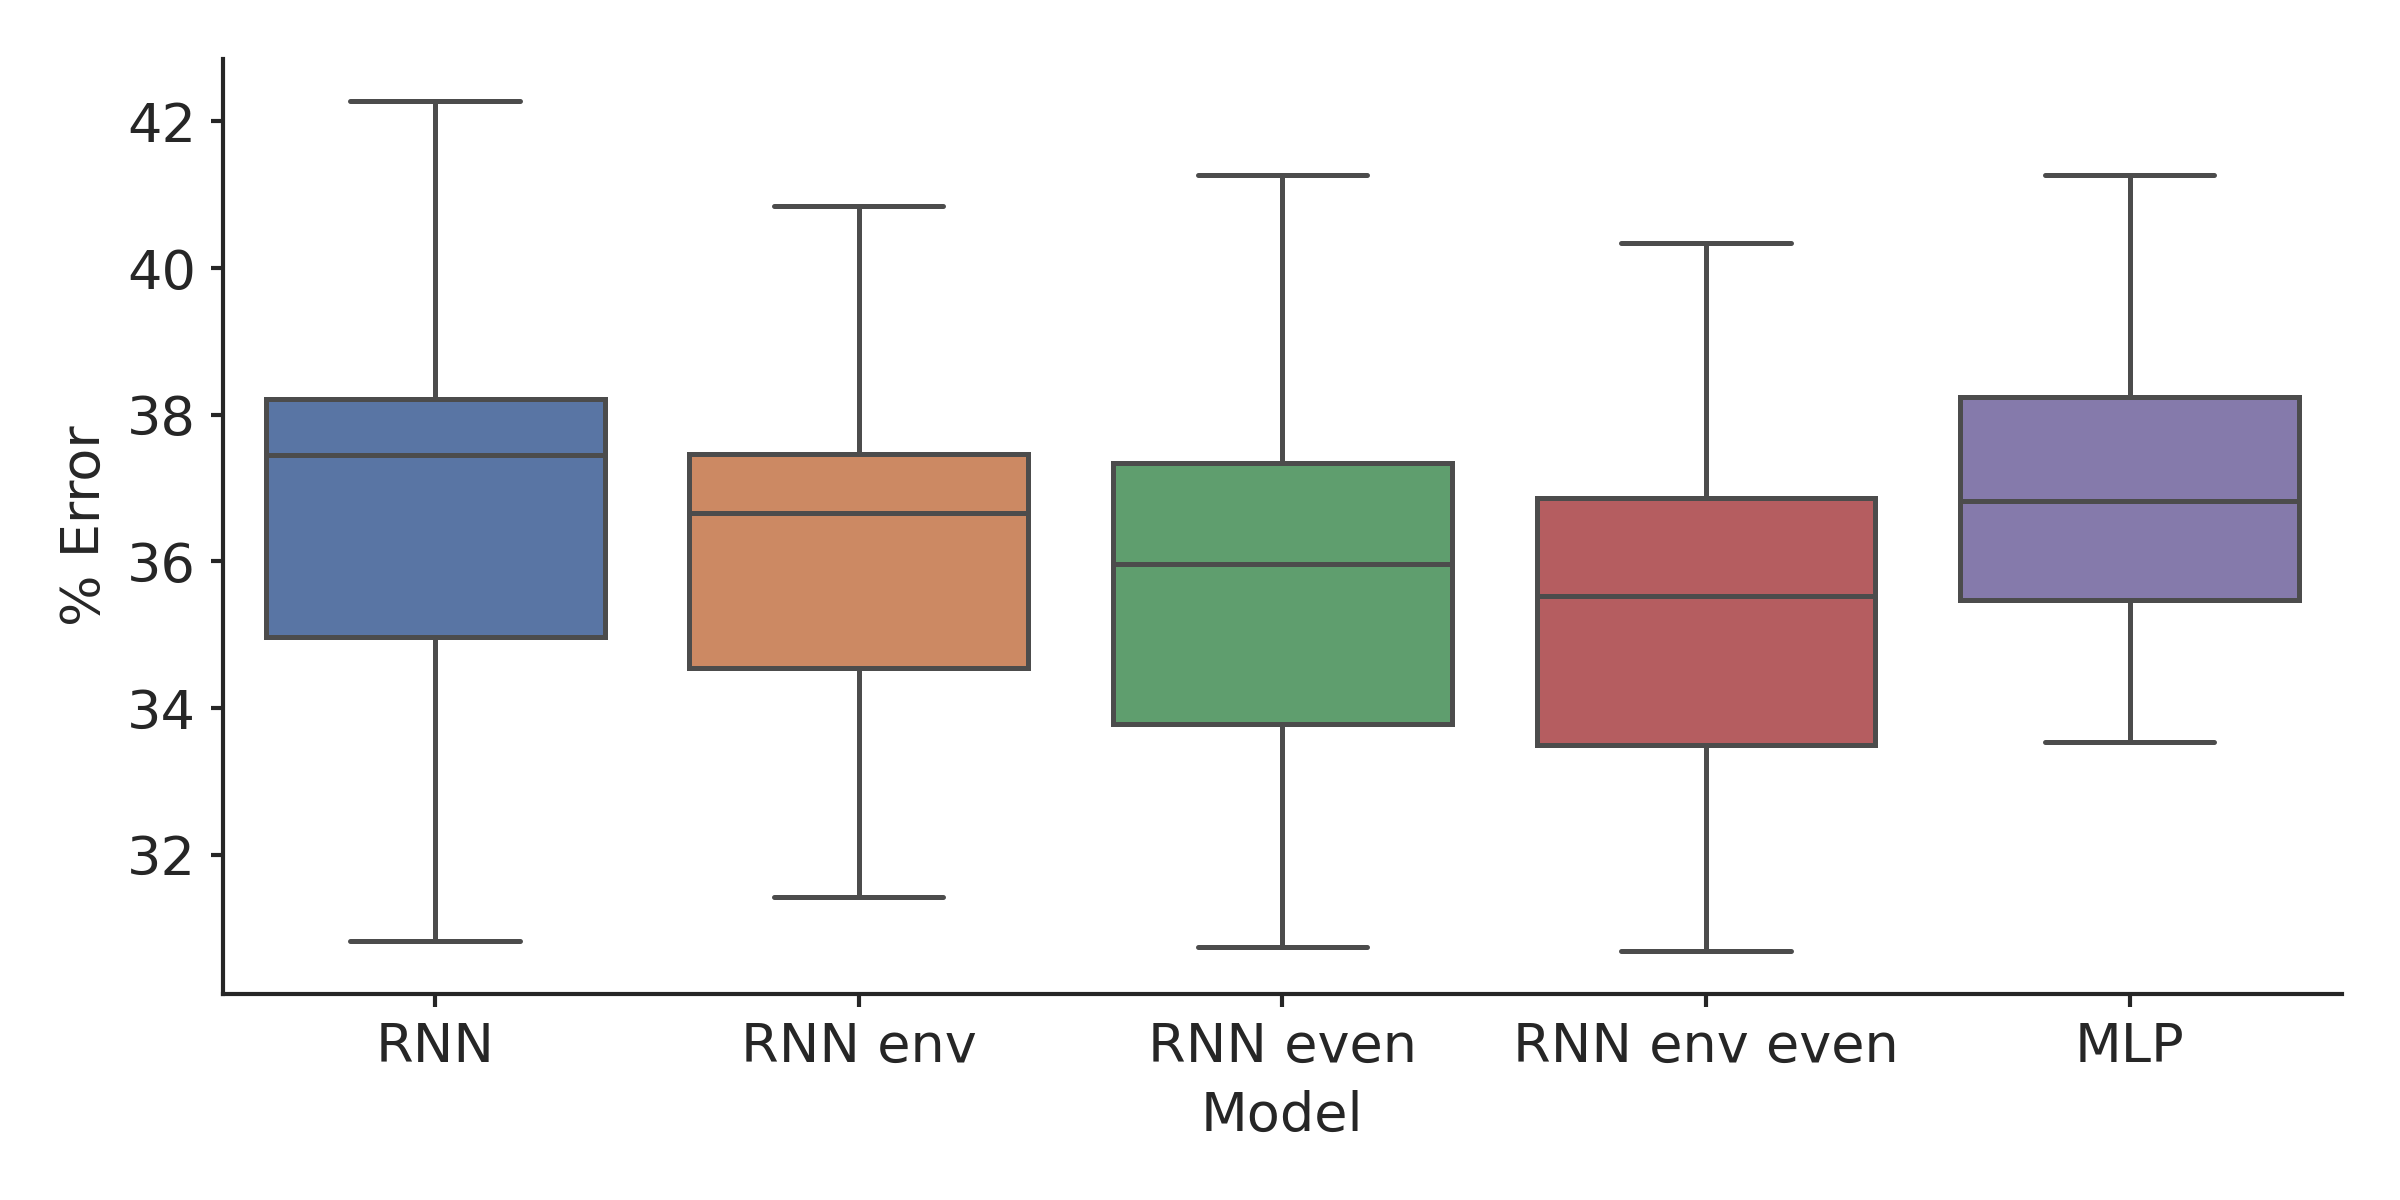
\includegraphics[width=.7\columnwidth]{images/chapter_3/performance_collapsed_33.png}
\caption[\textbf{Aggregated comparison of model performance}]{ Overall, the joint contribution of game events and environmental covariates appear to have a positive effect on performance. Box-plots show the 8-fold cross-validation performance expressed as the total percentage of error (i.e. SMAPE) of each model over the five targets.}
\label{model_comp_coll_33} 
\end{figure}

An interesting although surprising result was that the MLP architecture performed worse than the simple RNN architecture, despite having access to substantially more information (see Figure \ref{model_comp_expl_33}). Since this result was not expected a-priori and the estimated effect size is quite modest, we invite to interpret it with caution. Especially given the relatively small number of parameters assigned to the MLP architecture by the tuning procedure (see Figure \ref{model_comp_expl_33}).

\begin{table}[h]
\centering
\caption{Results of LMM on Collapsed Targets (Sum)}
\label{collapsed_lmm_33}
\begin{tabular}{ccccc}
\hline
\textbf{Model}           & \textbf{$\beta$} & \textbf{Z} & \textbf{p} & \textbf{95\% C.I.} \\ \hline
\multicolumn{5}{c}{\textbf{Collapsed Targets (Sum)}}                                                 \\ \hline
\textbf{Intercept (RNN)} & 36.518                & 41.374     & \textless .01   & 34.788 - 38.248      \\
\textbf{MLP}           & .366                 & 7.569     & \textless .01   & .271 - .460        \\
\textbf{RNN env}          & -.494                 & -1.224     & \textless .01   & -.589 - -.399        \\
\textbf{RNN even}            & -.938                 & -27.424     & \textless .01   & -1.419 - -1.230        \\
\textbf{RNN env even}             & -1.325                 & -19.414     & \textless .01   & -1.032 - -.843        \\ \hline
\end{tabular}
\end{table}

From the post-hoc analysis \ref{collapsed_post_hoc_33}, we can see how the hypotheses presented in section \ref{tuning_comparison_3} were confirmed for all architectures except MLP, which resulted to be the worst performing one (in some cases even by a substantial margin).

\begin{table}[h]
\centering
\caption{LMM Post-Hoc on Collapsed Targets (Sum)}
\label{collapsed_post_hoc_33}
\begin{tabular}{ccccc}
\hline
\textbf{Contrast}           & \textbf{$\beta_1$ - $\beta_2$} & \textbf{Z} & \textbf{p} & \textbf{95\% C.I.} \\ \hline
\multicolumn{5}{c}{\textbf{Collapsed Targets (Sum)}}                                                 \\ \hline
\textbf{Lag 1 - Median} & 2.528                & 20.210     & \textless .01   & 2.283 - 2.773      \\
\textbf{Median - ENet}          & 3.292                 & 26.322     & \textless .01   & 3.048 - 3.538        \\
\textbf{ENet - MLP}          & 2.778                 & 22.211     & \textless .01   & 2.533 - 3.024        \\ \hline
\end{tabular}
\end{table}

Figures \ref{model_comp_coll_game_33} and \ref{model_comp_coll_time_33} appear to show how including environmental and game events covariates seem to improve model performance in an additive fashion, with results that are consistent across temporal horizons

\begin{figure}[h]
\centering
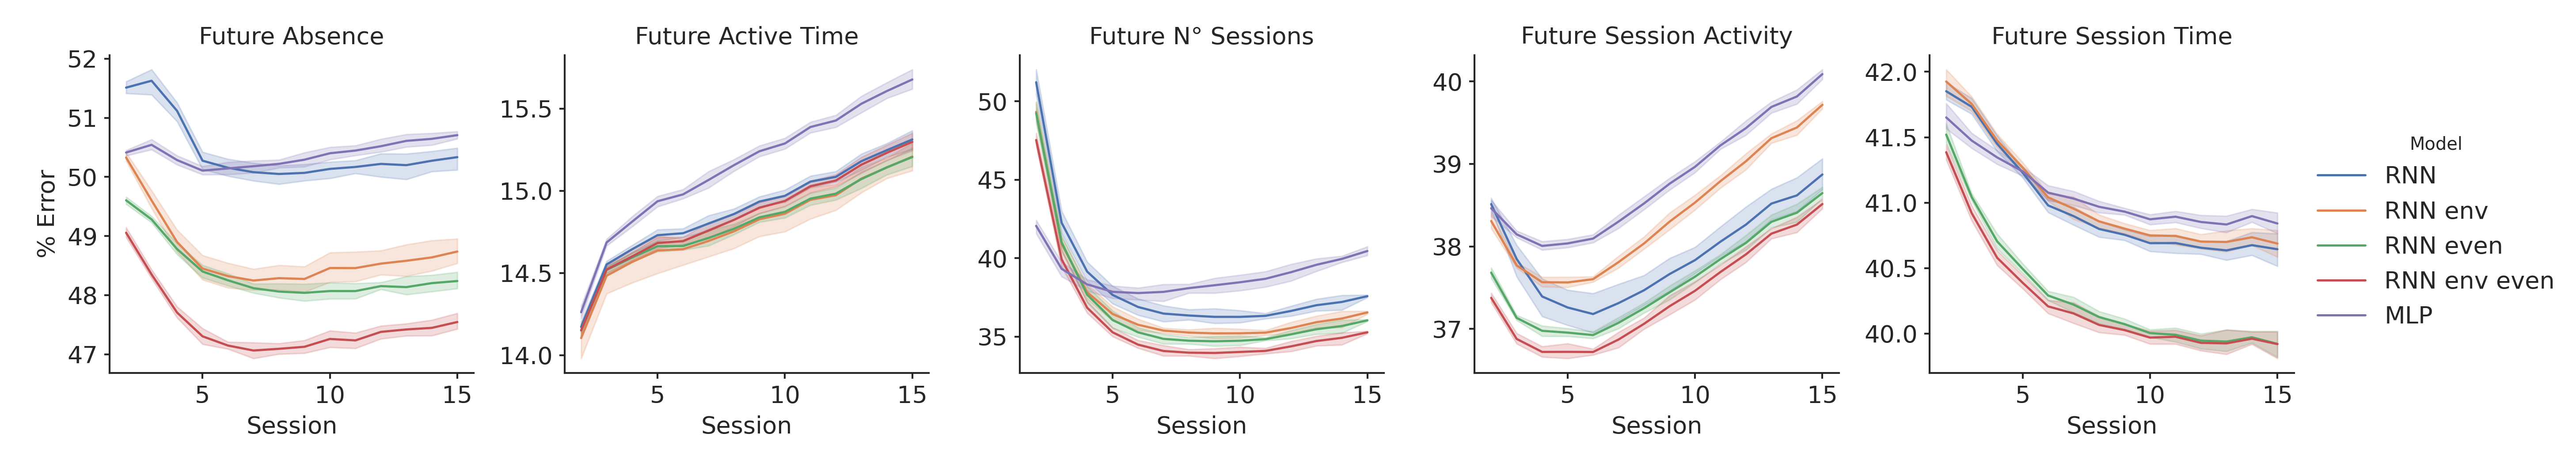
\includegraphics[width=\textwidth]{images/chapter_3/models_comparison_collapsed_game_33.png}
\caption[\textbf{Model comparison collapsing over game context}]{ Overall, including environmental and game events covariates appear to improve model performance in an additive fashion at every time horizon. The size of the improvement however seems to be heterogeneous across targets. Each column represent the performance of the considered models on a specific target. Solid lines indicate the expected \% error over time for a specific combination of target and model. Dashed areas indicate the standard error of the mean.}
\label{model_comp_coll_game_33}
\end{figure}

and game contexts. From the two figures we can also observe a number of relevant phenomena. 

First, the largest performance improvement was observed for the metric Future Absence. Second, as in the previous two model comparison iterations we can observe an heterogeneity in absolute performance driven by the game context and target taken into consideration. Third, the contribution of the environmental covariates on performance appeared to be rather erratic (occasionally even hurting performance) but always led to a consistent positive impact when coupled with game events information. Finally, despite the proposed modification to the RNN architecture had a consistent positive impact across the board, we can see from Figure \ref{model_comp_non_coll_33} that the effect of environmental and game events covariates alone appeared to vary across game contexts and targets.

\begin{figure}[h]
\centering
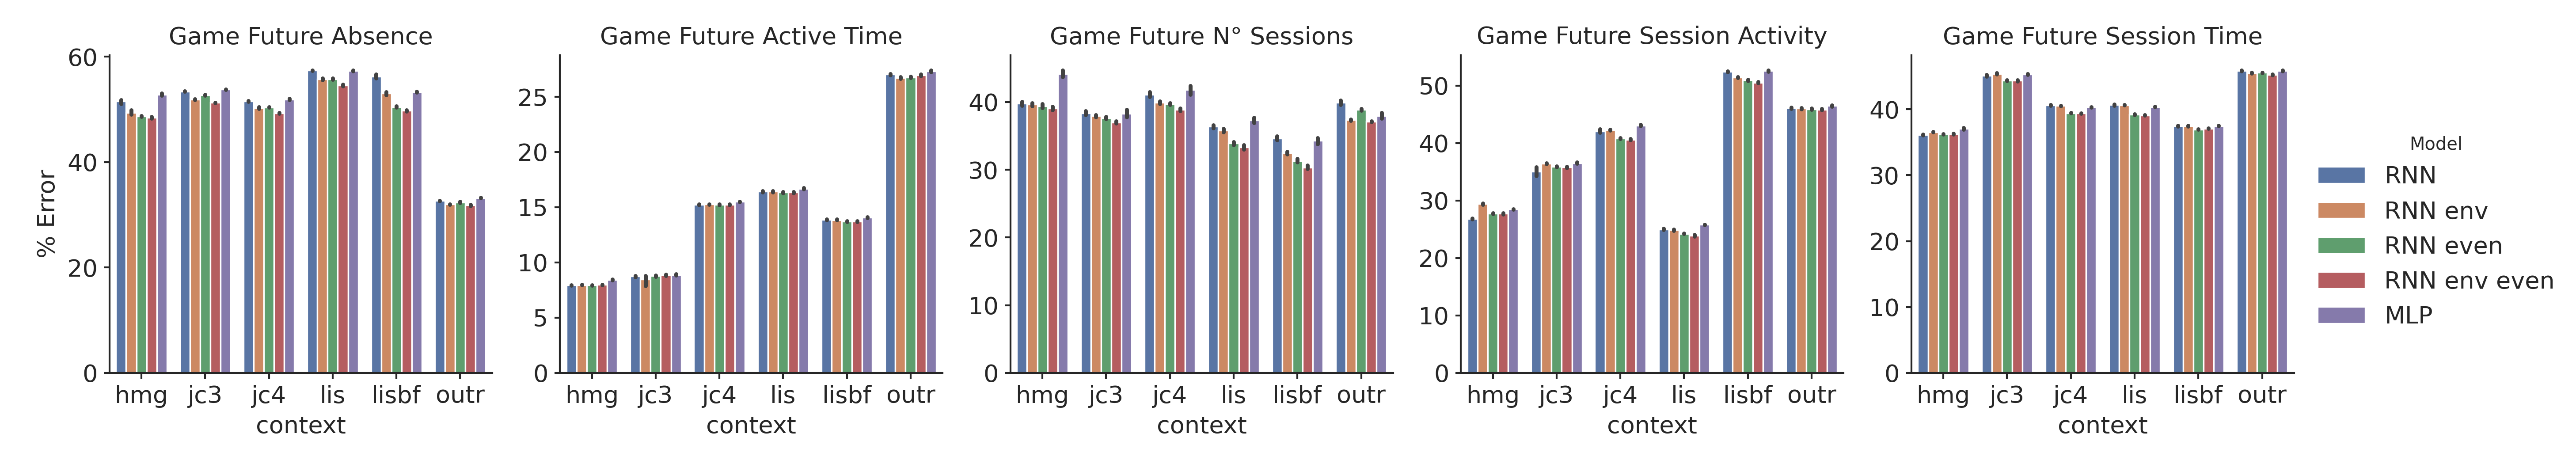
\includegraphics[width=\textwidth]{images/chapter_3/models_comparison_collapsed_time_33.png}
\caption[\textbf{Model comparison collapsing over time}]{Overall, including environmental and game events covariates appear to improve model performance in an additive fashion at every time horizon. The size of the improvement however seems to be heterogeneous across targets. Each column represent the performance of the considered models on a specific target. Bars indicate the expected \% error for a specific combination of game context, target and model. Black vertical lines indicate the standard error of the mean.}
\label{model_comp_coll_time_33} 
\end{figure}

This was confirmed by the analyses carried out at the target level, where a more heterogeneous performance landscape emerged. From table \ref{exploded_lmm_33} we can see that despite the inclusion of environmental and game events covariate improved the performance of the RNN architecture for most targets, there were some noticeable exceptions. 

For the target Future Active Time there seemed to be virtually no effect associated to the inclusion of the two covariates, this was likely due to marked performance differences between game contexts (see Figure \ref{model_comp_non_coll_33}). Consistently with previous findings, the MLP architecture appeared to under perform the simple RNN for all the considered targets.   

\begin{table}[h]
\centering
\caption{Results of LMM on Non-Collapsed Targets}
\label{exploded_lmm_33}
\begin{tabular}{ccccc}
\hline
\textbf{Model}  & \textbf{$\beta$} & \textbf{Z} & \textbf{p} & \textbf{95\% C.I.}                  \\ \hline

\multicolumn{5}{c}{\textbf{Future Absence}}                                                                         \\ \hline
\textbf{Intercept (RNN)} & 50.44                & 42.24     & \textless .01   & 48.10 - 52.78                     \\
\textbf{MLP}           & -.050                & -.845     & .398   & -.16 - .06                     \\
\textbf{RNN env}          & -1.74                & -29.30     & \textless .01   & -1.85 - -1.62                     \\
\textbf{RNN even}            & -2.93                & -49.34    & \textless .01   & -3.05 - -2.81                     \\
\textbf{RNN env even}             & -2.05                & -34.60     & \textless .01   & -2.17 - -1.94                       \\ \hline

\multicolumn{5}{c}{\textbf{Future Active Time}}                                                                     \\ \hline
\textbf{Intercept (RNN)} & 14.877                & 14.99      & \textless .01  & 12.93 - 16.82                     \\
\textbf{MLP}           & 0.26               & 6.65    & \textless .01  & .19 - .34                     \\
\textbf{RNN env}          & -.09                & -2.41     & .016  & -.17 - -.01                     \\
\textbf{RNN even}            & -.08                & -2.02     &  .043  & -.16 - -.002                     \\
\textbf{RNN env even}             & -.03                & -0.776      &  .438  & -.111 - .04                     \\ \hline

\multicolumn{5}{c}{\textbf{Future Session Time}}                                                                     \\ \hline
\textbf{Intercept (RNN)} & 40.978                & 77.831     & \textless .01  & 39.94 - 42.01                     \\
\textbf{MLP}            & .08                & 2.19     & .02  & .009 - .16                     \\
\textbf{RNN env}          & .05               & 1.28     & .2  & -.02 - .12                     \\
\textbf{RNN even}            & -.67                & -16.98     & \textless .01  & -.75 - .59                     \\
\textbf{RNN env even}             & -.73                & -18.48      & \textless .01  & -.81 - -.65                     \\ \hline

\multicolumn{5}{c}{\textbf{Future Session Activity}}                                                                 \\ \hline
\textbf{Intercept (RNN)} & 37.91                & 27.24     & \textless .01  & \multicolumn{1}{l}{35.18 - 40.64} \\
\textbf{MLP}            & .910                & 5.93     & \textless .01  & \multicolumn{1}{l}{.61 - 1.21} \\
\textbf{RNN env}          & .49                & 3.25     & \textless .01  & \multicolumn{1}{l}{.19 - .79} \\
\textbf{RNN even}            & -.32                & -2.091     & .03  & \multicolumn{1}{l}{.62 - -.02} \\
\textbf{RNN env even}             & -.51                & -3.35 & \textless .01  & \multicolumn{1}{l}{-.81 - -.21} \\ \hline

\multicolumn{5}{c}{\textbf{Future N° Sessions}}                                                                      \\ \hline
\textbf{Intercept (RNN)} & 38.37                & 73.91     & \textless .01  & 37.35 - 39.39                     \\
\textbf{MLP}            & .61                & 5.13     & \textless .01  & .37 - .84                     \\
\textbf{RNN env}          &  -1.17              & -9.89     & \textless .01  & -1.41 - -.94                     \\
\textbf{RNN even}            & -1.55                & -13.05     & \textless .01  & -1.78 - -1.32                     \\
\textbf{RNN env even}             & -2.41                & -20.24      & \textless .01  & -2.64 - -2.17                       \\ \hline
\end{tabular}
\end{table}

\begin{table}[h]
\centering
\caption{LMM Post-Hoc on Non-Collapsed Targets}
\label{exploded_post_hoc_33}
\begin{tabular}{ccccc}
\hline
\textbf{Contrast}  & \textbf{$\beta_1$-$\beta_2$} & \textbf{Z} & \textbf{p} & \textbf{95\% C.I.}                  \\ \hline
\multicolumn{5}{c}{\textbf{Future Absence}}                                                                         \\ \hline
\textbf{MLP - RNN env} & 1.69                & 28.458     & \textless .01   & 1.57 - 1.80                    \\
\textbf{MLP - RNN env even}           & 2.88                & 48.503     & \textless .01   & 2.76 - 3.00                     \\
\textbf{MLP - RNN even}           & 2.00                & 33.759     & \textless .01   &  1.89 - 2.12                     \\
\textbf{RNN env - RNN env even}           & 1.19                & 20.045     & \textless .01   & 1.07 - 1.30                     \\
\textbf{RNN env - RNN even}           & .31                & 5.301     & \textless .01   & .19 - .43                     \\
\textbf{RNN env even - RNN even}          & -.87                & -14.744     & \textless .01   & -.99 - -.76                    \\ \hline

\multicolumn{5}{c}{\textbf{Future Active Time}}                                                                     \\ \hline
\textbf{MLP - RNN env} & 0.36                & -11.305     & \textless .01   & 0.28 - 0.44                     \\
\textbf{MLP - RNN env even}           & 0.3                 & 42.461     & \textless .01   & 0.22 - 0.38                     \\
\textbf{MLP - RNN even}           & 0.35                & 42.461     & \textless .01   & 0.27 - 0.43                     \\
\textbf{RNN env - RNN env even}           & -0.06                & 42.461     & .1   & -0.14 - 0.01                     \\
\textbf{RNN env - RNN even}           & -0.01                & 42.461     &  .69   & -0.095 - 0.06                     \\
\textbf{RNN env even - RNN even}          & 0.05                & 6.438     &  .21   & -0.02 - 0.13                    \\ \hline

\multicolumn{5}{c}{\textbf{Future Session Time}}                                                                     \\ \hline
\textbf{MLP - RNN env} & -2.06                & -11.305     & \textless .01   & -2.42 - -1.70                     \\
\textbf{MLP - RNN env even}           & 7.76                & 42.461     & \textless .01   & 7.40 - 8.12                     \\
\textbf{MLP - RNN even}           & 7.76                & 42.461     & \textless .01   & 7.40 - 8.12                     \\
\textbf{RNN env - RNN env even}           & 7.76                & 42.461     & \textless .01   & 7.40 - 8.12                     \\
\textbf{RNN env - RNN even}           & 7.76                & 42.461     & \textless .01   & 7.40 - 8.12                     \\
\textbf{RNN env even - RNN even}          & 1.17                & 6.438     & \textless .01   & .81 - 1.535                    \\ \hline

\multicolumn{5}{c}{\textbf{Future Session Activity}}                                                                 \\ \hline
\textbf{MLP - RNN env} & -2.06                & -11.305     & \textless .01   & -2.42 - -1.70                     \\
\textbf{MLP - RNN env even}           & 7.76                & 42.461     & \textless .01   & 7.40 - 8.12                     \\
\textbf{MLP - RNN even}           & 7.76                & 42.461     & \textless .01   & 7.40 - 8.12                     \\
\textbf{RNN env - RNN env even}           & 7.76                & 42.461     & \textless .01   & 7.40 - 8.12                     \\
\textbf{RNN env - RNN even}           & 7.76                & 42.461     & \textless .01   & 7.40 - 8.12                     \\
\textbf{RNN env even - RNN even}          & 1.17                & 6.438     & \textless .01   & .81 - 1.535                    \\ \hline

\multicolumn{5}{c}{\textbf{Future N° Sessions}}                                                                      \\ \hline
\textbf{MLP - RNN env} & -2.06                & -11.305     & \textless .01   & -2.42 - -1.70                     \\
\textbf{MLP - RNN env even}           & 7.76                & 42.461     & \textless .01   & 7.40 - 8.12                     \\
\textbf{MLP - RNN even}           & 7.76                & 42.461     & \textless .01   & 7.40 - 8.12                     \\
\textbf{RNN env - RNN env even}           & 7.76                & 42.461     & \textless .01   & 7.40 - 8.12                     \\
\textbf{RNN env - RNN even}           & 7.76                & 42.461     & \textless .01   & 7.40 - 8.12                     \\
\textbf{RNN env even - RNN even}          & 1.17                & 6.438     & \textless .01   & .81 - 1.535                    \\ \hline

\end{tabular}
\end{table}

The results from the post-hoc analysis (see Table \ref{exploded_post_hoc_33}) partially validated our pair-wise hypotheses. No meaningful difference between architectures was found for the target Future Active Time. For all the other targets we observed that:

\begin{enumerate}
    \item The use of environmental covariates alone performed equally or worse than the use of game events alone.
    \item Combining the two type of covariates markedly outperformed the use of game events alone only for two targets: Future Absence and Future Number of Sessions
    \item The MLP architecture appeared to be the worst performing one.
\end{enumerate}

\begin{figure}[h]
\centering
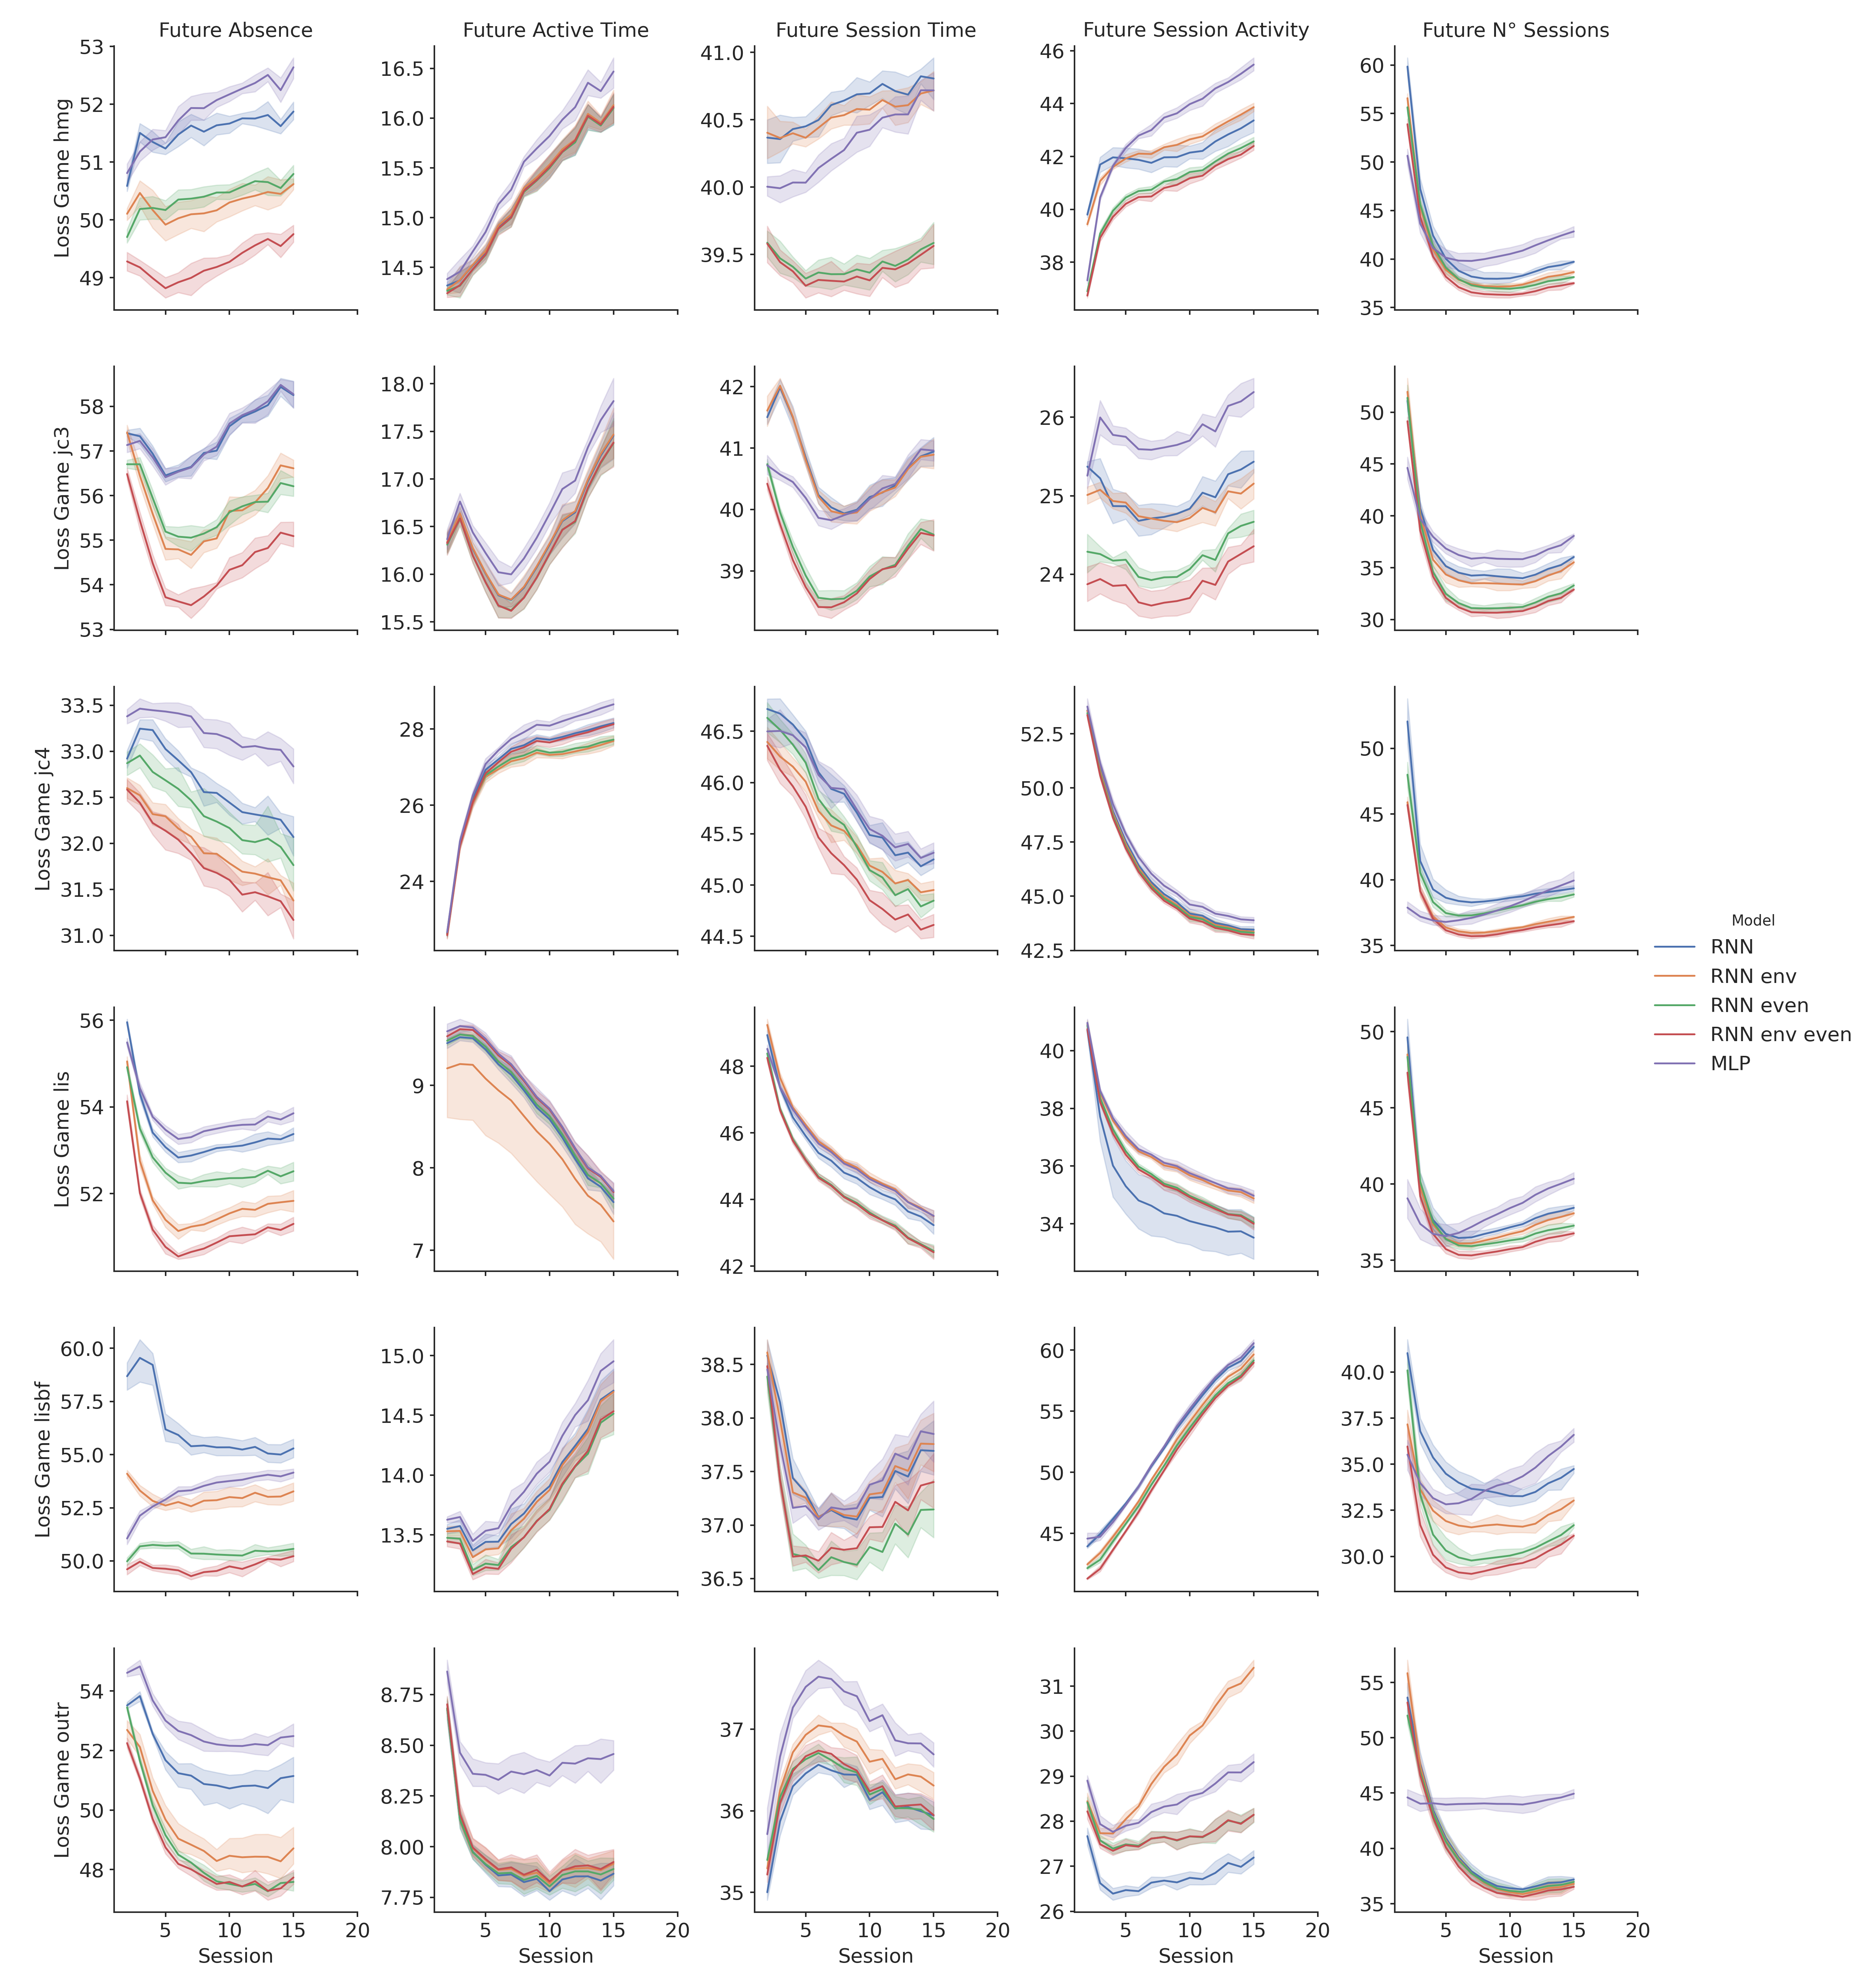
\includegraphics[height=0.7\textheight,keepaspectratio]{images/chapter_3/models_comparison_non_collapsed_33.png}
\caption[\textbf{Model comparison without collapsing}]{Overall, the joint contribution of game events and environmental covariates appear to have a positive effect of performance in most of the target-game context combinations and temporal horizons. Each column represents the performance of the considered models on a specific target while each row reports the performance on a specific game context. Solid lines indicate the expected \% error over time for a specific combination of target and model. Dashed areas indicate the standard error of the mean.}
\label{model_comp_non_coll_33} 
\end{figure}

From Figure \ref{model_comp_expl_33} we can see that, differently from the RNN architecture, the improvements in performance produced by the new covariates mechanisms required a substantial increase in the number of parameters and computation time. The MLP architecture again produced surprising results, despite having the least number of parameters it showed one of the highest computation time per epoch suggesting potential inefficiency during the fitting procedure.

\begin{figure*}[h]
\centering
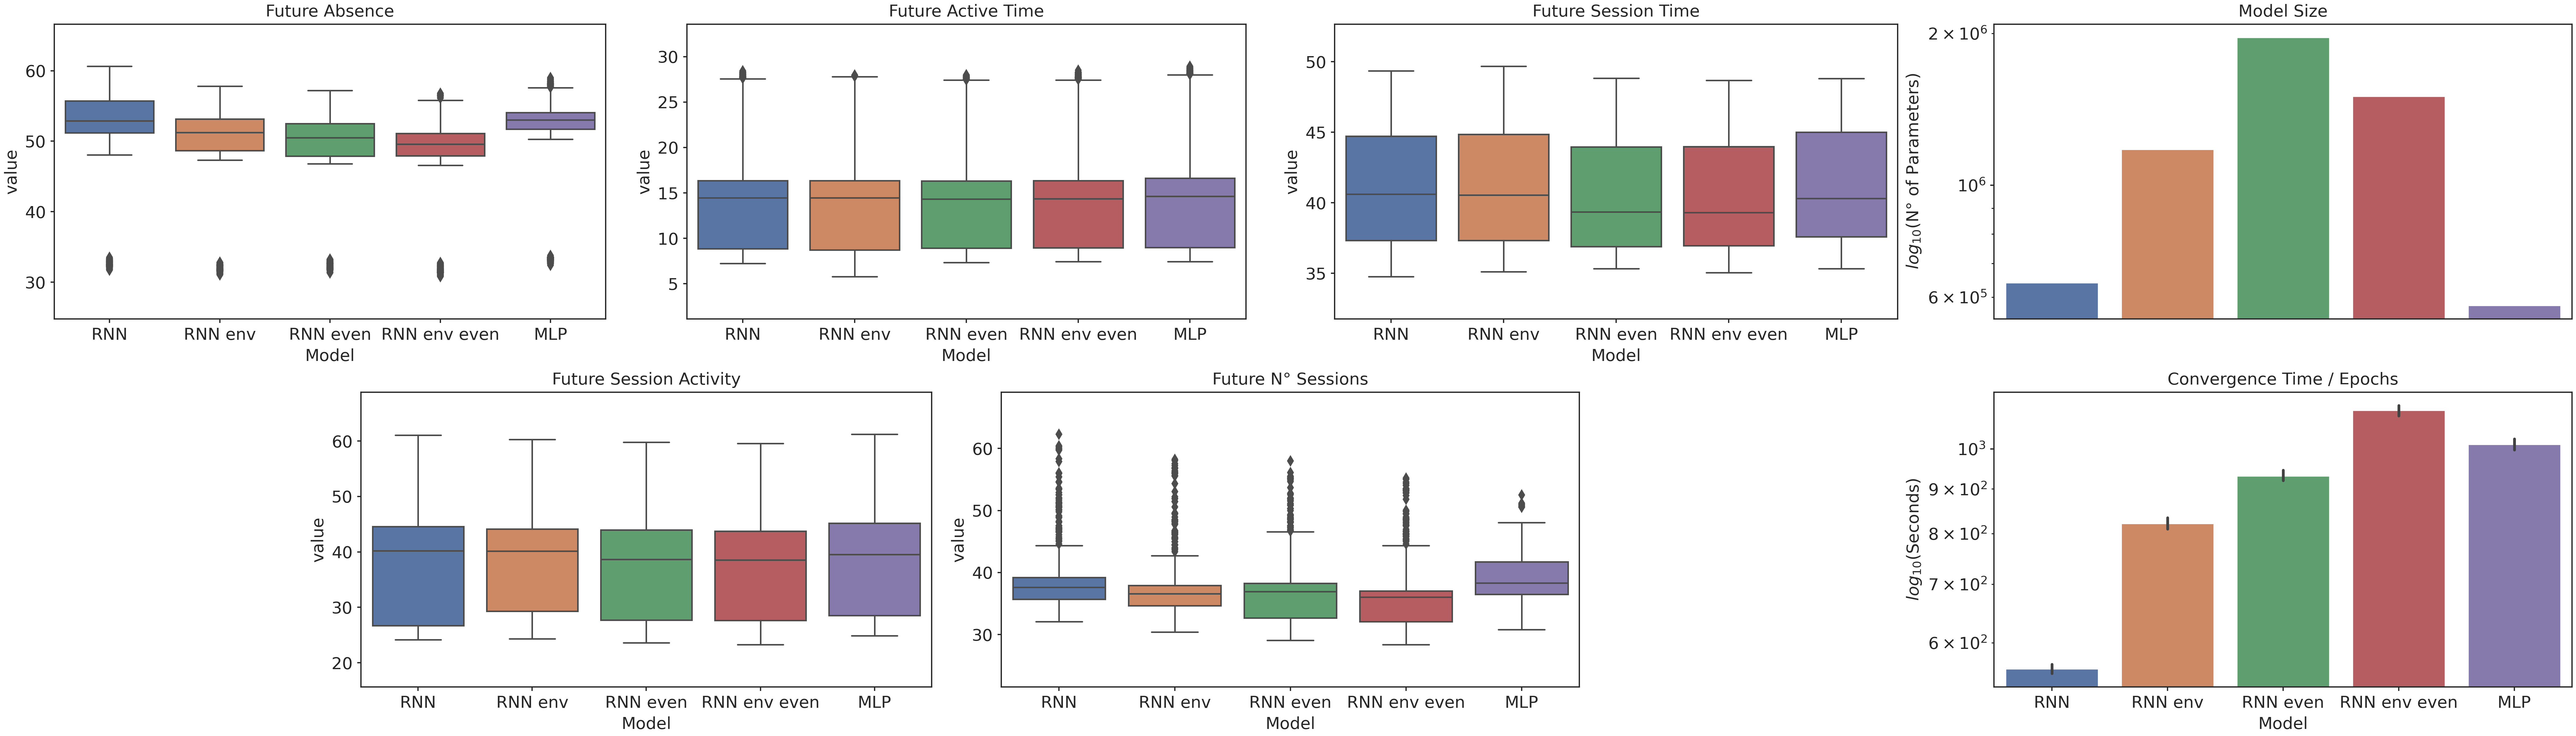
\includegraphics[width=\textwidth]{images/chapter_3/performance_exploded_33.png}
\caption[\textbf{Dis-aggregated comparison of models' performance}]{The combination of environmental and game events covariates appeared to improve performance in all the targets except Future Active Time. Box-plots show the 10-fold cross-validation performance expressed as percentage of error (i.e., SMAPE) of each model for the five targets. The bar-plot on the top row indicates the number of free parameters for each model while the bar plot on the bottom row shows the average time for each training epoch. Both bar-plots are $log_{10}$ scaled.}
\label{model_comp_expl_33} 
\end{figure*}

\section{Model Criticism}
\label{model_criticism_3}
Mirroring the results presented in sections \ref{results_1} and \ref{results_2} we were able to observe different level of performance in different game contexts and for different targets. This time however, the improvements provided by the specific variations of the RNN architecture were not homogeneous across contexts and targets, suggesting a slight inefficiency of the global multi-task approach. Overall most of the hypotheses introduced in section \ref{model_architecture_3} were confirmed by the model comparison results (at least at the aggregate level). From this we can derive a series of conclusions on the effectiveness of the different architectures in generating a latent representation with adequate predictive powers.

\begin{enumerate}
    \item Considering changes in the surrounding environment might only marginally contribute to the predictive perfromance.
    \item Considering the characteristics of the object can have a greater impact on the predictive accuracy.
    \item In line with the what presented in chapters \ref{chapter_lit_review} and \ref{chapter_theory_modelling}, the combination of the two covariates provides the most effective strategy for producing accurate predictions.
    \item Despite the poor performance of the MLP architecture should be interpreted with caution, it strengthens the idea that dynamic operations are important for computing the latent representation.
\end{enumerate}

We want to stress that despite the proposed architectures improved upon the limitations of their predecessor, the largest effects have been observed mostly at the aggregated level or for some particular combinations of game contexts and targets. This might have been caused by either a true inefficiency of the proposed architectures or by a less thorough an ineffective hyper parameter tuning. Indeed, the inclusion of environmental and game events covariates substantially increased the number of degrees of freedom available for defining the architectures. In this view, the budged provided to the Hyperband algorithm might have not been sufficient for individuating the best hyper-parameters configuration ultimately leading to a sub-optimal performance. 

In addition to the technical criticalities that we just described we can also individuate a number of methodological ones. First and foremost, we have to stress how the goal of this model building exercise has always been to create a methodology for approximating the latent state described by the work of McClure \textit{et. al.} \cite{mcclure2003computational} and Zhang \textit{et. al.} \cite{zhang2009neural}. In this regard, our approach was formally different from that of TD Learning \footnote{See \cite{barto2004reinforcement} for a review of the differences between supervised and reinforcement learning.} and did not model the process of incentive salience attribution but rather attempted to approximate the product of this process (i.e., changes in attributed incentive salience). For this reason a direct comparison with the work of McClure \textit{et. al.} \cite{mcclure2003computational} and Zhang \textit{et. al.} \cite{zhang2009neural} is difficult. 

Moreover, unlike TD learning \cite{schultz1997neural} our model is not guaranteed to converge on a quantification of $V$ that is directly comparable to its biological counterpart or that has arisen from the same type of computations. This is also reinforced by the differences in mechanistic functioning between biological and artificial neural networks \cite{lillicrap2019backpropagation,lillicrap2020backpropagation}. These issues are partially attenuated by the constraints provided by our theoretical framework but in line with similar reports in the literature \cite{calhoun2019unsupervised,wang2018prefrontal} a verification based on controlled experiments is desirable. 

Differently from the works of Calhoun \textit{et. al.} \cite{calhoun2019unsupervised},  McClure \textit{et. al.} \cite{mcclure2003computational} and Zhang \textit{et. al.} \cite{zhang2009neural}, our methodology relied on a  supervised learning approach to perform both prediction of future behaviour and latent state estimation, making this two tasks infeasible before any data was observed. This limitation could be attenuated by initializing our model using a representation  generated in an unsupervised manner. 

The model comparison step in our experimental pipeline lacked of an important control condition: an architecture with linear recurrent operations. Indeed, despite we were able to assert the superiority of the combination of non-linearity and recurrency, we could not evaluate the impact of recurrency alone. Since the LSTM operation relies on non-linearity for both state generation and information filtering, we could not foresee which impact its removal could have had, hence we preferred to not burden with an additional architecture an already demanding part of the experimental pipeline. Future works should aim to clarify the contribution of recurrency alone on predictive accuracy and representation generation. 

Lastly, despite our approach appeared to deal gracefully  with objects having different structural characteristics (i.e., different in-game characteristics), these were limited to the domain of video games. In order to verify the generalizability of our approach, future work should include data generated from a variety of contexts (e.g. web services, online and laboratory-based experiments).

\section{Discussion}
\label{discussion_3}
In this chapter we focused on implementing and validating the predictive model designed in chapter \ref{chapter_theory_modelling}. This was done through an iterative approach that allowed us to construct, in a principled way, solutions of increasing complexity while also empirically test some of the theoretical assumptions introduced in chapters \ref{chapter_lit_review} and \ref{chapter_theory_modelling}. 

We showed that metric quantifying the strength of interactions between a group of individuals and a set of potentially rewarding objects can be effectively used by a computational model for predicting the intensity of future ones. A finding that is in line with a long tradition of experimental results in behavioural psychology \cite{thorndike1927law, skinner1953science} and neuroscience \cite{schultz1997neural, berridge2004motivation}. 

We also showed how a single global model can be used for generating these predictions across a wide range of objects. This idea resonates with the concepts of motivation and engagement as presented in chapter \ref{chapter_lit_review}: single overarching processes able to describe and predict how strongly an individual will interact with an object. 

It appeared evident that in order to produce more accurate predictions it was important to consider the full history of previous interactions rather summarizing them using a small number of descriptive metrics. From this, we can derive that for estimating constructs that are dynamic in nature (e.g., latent states like the level of attributed saliency), we must rely on data that reflect the characteristics of the process that generated them. In particular, this appeared to extend also to the type of computations performed by the model used for estimation. For instance, in our case we showed that techniques able to represent complex non-linear temporal dynamics in the data outperformed competing approaches, even when these had comparable computational power and expressiveness (i.e., architectures relying on feedforward operations). As we highlighted in chapter \ref{chapter_theory_modelling}, this is in line with the dynamical nature of motivation, incentive salience attribution and, by extension, engagement which can often be considered a temporal processes with memory \cite{toates1994comparing,robinson1993neural,zhang2009neural,tindell2009dynamic,berridge2012prediction}. Indeed, results from computational studies suggest that the attribution of value and saliency to potentially rewarding objects or actions is often carried out by non-linear recurrent operations \cite{song2017reward,wang2018prefrontal} and that ANN with recurrent connections are well suited for approximating these operations \cite{kietzmann2018deep}. 

Finally we were able to partially support the idea that considering only information on the intensity of interactions was a limiting factor preventing the generation of latent representations with higher predictive powers. We showed how incorporating information on the characteristics of the objects and and the environment in which the interactions occurred improved, even if marginally, the accuracy of the model during the predictive task. These results are in line with findings in the literature showing how in-game mechanics are the source of the rewarding experience generated during the playing activity \cite{westwood2010role,king2010role,king2010video,yannakakis2013player,phillips2013videogame} and hence directly involved in its maintenance. 

It is important to highlight that in this chapter we used model selection and predictive accuracy mostly as a device for testing hypotheses and guiding us towards the most promising approach for generating good approximations of the constructs we were trying to model. In this view, the next chapter will focus on extracting, visualizing and analyzing the representations produced by the RNN architecture and by its derivatives. This will be done in order to evaluate how these representations vary within and between models and to verify if they show a set of functional characteristics proper of attributed incentive salience. For doing so we will try to map the information embedded in the high dimensional representations generated by our ANN architectures back to the lower dimensional space of observed behaviour. 
